\documentclass[preprint,aps,pra,onecolumn]{revtex4-1} %reprint
%\tightenlines

%\draft
\usepackage{etex}
\usepackage{amsmath}
\usepackage{bm}
\usepackage{bbm}
\usepackage{listings}
% % \textwidth 16cm \textheight 23.5cm
% \renewcommand{\baselinestretch}{1.2}
\usepackage{graphicx}
\usepackage{graphics}
\usepackage{epsfig}
\usepackage{color}
\usepackage{multirow}
\usepackage[colorlinks]{hyperref}
\usepackage{fancyhdr}
\usepackage{calc}
\usepackage{natbib} %[numbers]
\usepackage{bibentry}
% underline tool
\usepackage[normalem]{ulem}
\usepackage{xcolor}
%\uline{foo}	Underlines foo
%\uuline{foo}	Double underlines foo
%\uwave{foo}	Underlines foo with a wavy line
%\sout{foo}	Strikesout foo
%\xout{foo}	Crosses out foo with ¡®/6¤7¡¯
% triple lines in colors
\makeatletter
\newcommand\uuuline{\bgroup\markoverwith%
   {%
     \textcolor{red}{\rule[-0.5ex]{2pt}{0.4pt}}%
     \llap{\textcolor{blue}{\rule[-0.7ex]{2pt}{0.4pt}}}%
     \llap{\textcolor{green}{\rule[-0.9ex]{2pt}{0.4pt}}}%
   }%
   \ULon}
\makeatother


\usepackage{amsmath,soul} % underline with a number
% usage example: $\underset{4}{\text{\ul{This is short text}}}$
% another package to use, but did not work for me.
% From: http://tex.stackexchange.com/questions/45341/labeling-underlined-text-over-multiple-lines
%\usepackage{soulpos}
%\ulposdef{\ulnumaux}{%
%   $\underset{\saveulnum}{\rule[-.7ex]{\ulwidth}{.4pt}}$}
%
%\newcommand{\ulnum}[2]{%
%  \def\saveulnum{#1}%
%  \ulnumaux{#2}}

% todo list and commands
\usepackage{todonotes}
%% to avoid the conflict with amths package % not working
%\makeatletter
%\providecommand\@dotsep{5}
%\makeatother
%\listoftodos\relax
\usepackage{makeidx}
\allowdisplaybreaks
% for eps transfering to pdf.
\usepackage[update,prepend]{epstopdf}
\usepackage{ifpdf}

\ifpdf
   \usepackage{graphicx}
   \usepackage{epstopdf}
   \epstopdfsetup{suffix=}
   \DeclareGraphicsRule{.eps}{pdf}{.pdf}{`epstopdf #1}
   \pdfcompresslevel=9
\else
   \usepackage{graphicx}
\fi
% subfig
%\usepackage{mwe}
\usepackage{subfig}
% to fix a figure's position using [H] option of thec figure.
\usepackage{float}
% to use \lesssim and other math symbols
\usepackage{amssymb}


% self-defined short-cuts and commands

% packages we need for judging the operating system
% compile your tex file with option -shell-escape is required: 
% e.g. xelatex -shell-escape file.tex
\usepackage{pdftexcmds}
\usepackage{catchfile}
\usepackage{ifluatex}
\usepackage{ifplatform}

% self-definition for short hand

% symbols and math operators
\DeclareMathOperator{\spn}{span}
\DeclareMathOperator{\tr}{tr}
% definition of grammars % formats related
\definecolor{MyDarkGreen}{rgb}{0.0,0.4,0.0}
\newcommand{\greek}[1]{{\selectlanguage{greek}#1}} % will look for grmn font: tlmgr install cbfonts (65 MB)

% functions
\newcommand{\sn}{\mathrm{sn}}
\newcommand{\cn}{\mathrm{cn}}
\newcommand{\dn}{\mathrm{dn}}

% constants
\newcommand{\invtpi}{\frac{1}{2\pi}}

% vectors and tensors
\def\en{\mathbf{e}_n}
\def\eye{\mathbf{I}}
\newcommand\lvec[1]{\accentset{\leftarrow}{#1}}
% math font
\newcommand{\bmc}[1]{\boldsymbol{\mathcal{#1}}}

% derivatives and integrals
% ordinary derivatives
\newcommand{\drv}{\mathrm{d}}
\newcommand{\dt}[1]{\frac{{\mathrm d} {#1}}{{\mathrm d}t}}
\newcommand{\dx}[1]{\frac{{\mathrm d} {#1}}{{\mathrm d}x}}
\newcommand{\dtau}{\frac{{\mathrm d} }{{\mathrm d}\tau}}
\newcommand{\dd}[2]{\frac{{\mathrm d} {#1}}{{\mathrm d} {#2}}}
\newcommand{\sdt}[1]{\frac{{\mathrm d}^2 {#1}}{{\mathrm d}t^2}}
\newcommand{\sdx}[1]{\frac{{\mathrm d}^2 {#1}}{{\mathrm d}x^2}}
\newcommand{\sdd}[2]{\frac{{\mathrm d}^2 {#1}}{{\mathrm d}{#2}^2}}
\newcommand{\ddn}[3]{\frac{{\mathrm d}^{#1} #2}{{\mathrm d} #3 ^{#1}}}

% partial derivatives
\newcommand{\pt}[1]{\frac{\partial {#1}}{\partial t}}
\newcommand{\px}[1]{\frac{\partial {#1}}{\partial x}}
\newcommand{\pp}[2]{\frac{\partial {#1}}{\partial {#2}}}
\newcommand{\spt}[1]{\frac{\partial^2 {#1}}{\partial t^2}}
\newcommand{\spx}[1]{\frac{\partial^2 {#1}}{\partial x^2}}
\newcommand{\spp}[2]{\frac{\partial^2 {#1}}{\partial {#2}^2}}
\newcommand{\ppn}[3]{\frac{\partial^{#1} #2}{\partial #3 ^{#1}}}
% integrals
\newcommand{\intl}[2]{\int_0^\infty\! #1 \mathrm{d}#2}
\newcommand{\intf}[2]{\int_{-\infty}^\infty\! #1 \mathrm{d}#2}


% quantum operators
\newcommand{\ssp}{\braket{\sigma^{+}(t)\sigma^{-}(t)}}
\newcommand{\aap}{\braket{a^{\dagger}(t)a(t)}}
\newcommand{\as}{\braket{a^{\dagger}(t)\sigma^{-}(t)}}
\newcommand{\sa}{\braket{a(t)\sigma^{+}(t)}}
\newcommand{\Hssp}{\braket{\sigma^{+}\sigma^{-}}}
\newcommand{\Haap}{\braket{a^{\dagger}a}}
\newcommand{\Has}{\braket{a^{\dagger}\sigma^{-}}}
\newcommand{\Hsa}{\braket{a\sigma^{+}}}
\newcommand{\adag}{a^{\dagger}}
\newcommand{\sigm}{\sigma^{-}}
\newcommand{\sigp}{\sigma^{+}}
\newcommand{\sigz}{\sigma^{z}}
\newcommand{\gp}{\gamma^{\prime}}
\newcommand{\oal}{\omega_a-\omega_0}
\newcommand{\ocl}{\omega_c-\omega_0}


% Green function related
\def\GFT{\overline{\bf G}}
\def\IT{\overline{\bf I}}
\def\TT{\overline{\bf T}}
\def\MT{\overline{\bf M}}
\def\AT{\overline{\bf A}}
\def\BT{\overline{\bf B}}
\def\fT{\overline{\bf f}}
\def\LT{\overline{\bf L}}
\def\alphaT{\overline{\bf \alpha}}
\def\GFTr{\overline{\bf G}\left(\mathbf{r},\mathbf{r}'\right)}
\def\GFTrw{\overline{\bf G}\left(\mathbf{r},\mathbf{r}';\omega\right)}
\def\rarg{\left(\mathbf{r}\right)}
\def\rargw{\left(\mathbf{r};\omega\right)}
\def\rrarg{\left(\mathbf{r},\mathbf{r}'\right)}
\def\rrargw{\left(\mathbf{r},\mathbf{r}';\omega\right)}
\def\rk{\left(\mathbf{r}_k\right)}
\def\rn{\left(\mathbf{r}_n\right)}
\def\rnrn{\left(\mathbf{r}_n,\mathbf{r}_n\right)}
\def\rnrk{\left(\mathbf{r}_n,\mathbf{r}_k\right)}
\def\rkrk{\left(\mathbf{r}_k,\mathbf{r}_k\right)}
\def\rkrn{\left(\mathbf{r}_k,\mathbf{r}_n\right)}
\def\br{\mathbf{r}}
\def\Erw{\hat{\mathbf{E}}(\mathbf{r},\omega)}
\def\E0{\hat{\mathbf{E}}^{(0)}(\mathbf{r},\omega)}
\def\Arw{\hat{\mathbf{A}}(\mathbf{r},\omega)}
\def\Snw{\hat{\mathbf{S}}_n(\omega)}
\def\Unw{\mathbf{U}_n(\omega)}
\def\unw{U_n(\omega)}
\def\Alphanw{{\bm \alpha}_n(\omega)}
\def\Krrw{\mathbf{K}(\mathbf{r},\mathbf{r}',\omega)}
\def\Krrnw{\mathbf{K}(\mathbf{r},\mathbf{r}_n,\omega)}
\def\GTrrw{\mathbf{G}^T(\mathbf{r},\mathbf{r}',\omega)}
\def\Grrw{\mathbf{G}(\mathbf{r},\mathbf{r}',\omega)}
\def\Gn{\mathbf{G}^n}
\def\Gm1{\mathbf{G}^{n-1}}
\def\GN{\mathbf{G}^N}
\def\G0{\mathbf{G}^0}
\def\G1{\mathbf{G}^1}
\def\Gi{\mathbf{G}^i}
\def\flamr{\mathbf{f}_\lambda(\mathbf{r})}
\def\rrn{\mathbf{r},\mathbf{r}_n}
\def\rnrn{\mathbf{r}_n,\mathbf{r}_n}
\def\rr{\mathbf{r},\mathbf{r}'}


% braket.sty          Macros for Dirac bra-ket <|> notation and sets {|}
%
\def\bra#1{\langle{#1}\rvert}%{\mathinner{\langle{#1}\rvert}}
\def\ket#1{\lvert{#1}\rangle}%{\mathinner{\lvert{#1}\rangle}}
\def\braket#1{\mathinner{\langle{#1}\rangle}}
\def\Bra#1{\left<#1\right|}
\def\Ket#1{\left|#1\right>}
{\catcode`\|=\active
  \gdef\Braket#1{\left<\mathcode`\|"8000\let|\BraVert {#1}\right>}}
\def\BraVert{\egroup\,\mid@vertical\,\bgroup}
{\catcode`\|=\active
  \gdef\set#1{\mathinner{\lbrace\,{\mathcode`\|"8000\let|\midvert #1}\,\rbrace}}
  \gdef\Set#1{\left\{\:{\mathcode`\|"8000\let|\SetVert #1}\:\right\}}}
\def\midvert{\egroup\mid\bgroup}
\def\SetVert{\egroup\;\mid@vertical\;\bgroup}
% Some stuff deleted
% Macros for Dirac bra-ket <|> notation
%\def\bra#1{\mathinner{\langle{#1}|}}
%\def\ket#1{\mathinner{|{#1}\rangle}}
\def\Braket#1#2{\mathinner{\langle{#1}\! \mid\! {#2} \rangle}}
\def\ketbra#1{\ket{#1}\!\!\bra{#1}}
\newcommand{\Ketbra}[2]{\ket{#1}\!\!\bra{#2}}
\def\sandwich#1#2{\bra{#1}\! #2 \! \ket{#1}}
\def\Sandwich#1#2#3{\bra{#1}\! #2\! \ket{#3}}
%
% END  braket.sty     Macros for Dirac bra-ket <|> notation and sets {|}


%% Ben's shortcuts.
% Equation, citation, and labeling macros
%========================================================================================
\newcommand{\erf}[1]{Eq.~(\ref{#1})}
\newcommand{\frf}[1]{Fig.~\ref{#1}}
\newcommand{\srf}[1]{Sec.~\ref{#1}}
\newcommand{\nn}{\nonumber}
\newcommand{\mbf}[1]{\mathbf{#1}}
%========================================================================================
% General quantum mechanics macros
%========================================================================================
\newcommand{\ip}[2]{\langle{#1}|{#2}\rangle}
\newcommand{\op}[2]{\ket{#1}\bra{#2}}
\newcommand{\enavg}[1]{\mathrm{E}\sq{#1}}
\newcommand{\gravg}[1]{\mathbb{E}\sq{#1}}
\newcommand{\expt}[1]{\langle{#1}\rangle}
\newcommand{\dg}{^\dagger}
\newcommand{\smallfrac}[2]{\mbox{$\frac{#1}{#2}$}}
\newcommand{\emn}[1]{ \mathbbm{E}_{#1} }
\newcommand{\Tr}{\mbox{Tr}}
%\newcommand{\tensor}[1]{\boldsymbol{#1}}%{\overset{\leftrightarrow}{#1}}
%========================================================================================
% Famous physicists
%========================================================================================
\newcommand{\sch}{Schr\"odinger}
\newcommand{\hei}{Heisenberg }
\newcommand{\ein}{Einstein }
\newcommand{\str}{Stratonovich }
%========================================================================================
% Dirac notation and commutators
%========================================================================================
\newcommand{\norm}[1]{\lvert #1 \rvert}
\newcommand{\opnorm}[1]{\lVert #1 \rVert}
%\newcommand{\ket}[1]{\lvert #1 \rangle}
%\newcommand{\bra}[1]{\langle #1 \rvert}
\newcommand{\bravket}[2]{\langle\, #1\,\vert\, #2 \,\rangle}
\newcommand{\av}[1]{\left\langle #1 \right\rangle}
\newcommand{\proj}[1]{\ket{#1}\!\bra{#1}}
\newcommand{\commut}[2]{[\ssp #1,\,#2\ssp]}
\newcommand{\anticommut}[2]{\{\ssp #1,\,#2\ssp\}}
% big Dirac notation and commutators
\newcommand{\bnorm}[1]{\big\lvert #1 \big\rvert}
\newcommand{\bopnorm}[1]{\big\lVert #1 \big\rVert}
\newcommand{\bket}[1]{\big\lvert\, #1\, \big\rangle}
\newcommand{\bbra}[1]{\big\langle\, #1\, \big\rvert}
\newcommand{\bbraket}[2]{\big\langle\, #1\,\big\vert\, #2 \,\big\rangle}
\newcommand{\bav}[1]{\bigl\langle #1 \bigr\rangle}
\newcommand{\bproj}[1]{\bket{#1}\!\bbra{#1}}
\newcommand{\bcommut}[2]{\big[\ssp #1,\,#2\ssp\big]}
\newcommand{\banticommut}[2]{\big\{\ssp #1,\,#2\ssp\big\}}
% Big Dirac notation and commutators
\newcommand{\Bnorm}[1]{\Big\lvert #1 \Big\rvert}
\newcommand{\Bopnorm}[1]{\Big\lVert #1 \Big\rVert}
\newcommand{\Bket}[1]{\Big\lvert\, #1\, \Big\rangle}
\newcommand{\Bbra}[1]{\Big\langle\, #1\, \Big\rvert}
\newcommand{\Bbraket}[2]{\Big\langle\, #1\,\Big\vert\, #2 \,\Big\rangle}
\newcommand{\Bav}[1]{\Bigl\langle #1 \Bigr\rangle}
\newcommand{\Bproj}[1]{\Bket{#1}\!\Bbra{#1}}
\newcommand{\Bcommut}[2]{\Big[\ssp #1,\,#2\ssp\Big]}
\newcommand{\Banticommut}[2]{\Big\{\ssp #1,\,#2\ssp\Big\}}
%========================================================================================
% Nanofiber interface macros
%========================================================================================
\newcommand{\expect}[1]{\big\langle #1 \big\rangle}
\newcommand{\expects}[1]{\langle #1 \rangle}
\newcommand{\melement}[3]{\langle #1 \lvert #2 \rvert #3 \rangle}
\newcommand{\Ip}[2]{\left\langle {#1},{#2} \right\rangle}
\newcommand{\modsq}[1]{\lvert #1 \rvert^2}
\newcommand{\normsq}[1]{\lVert #1 \rVert^2}
\newcommand{\grad}{\nabla}
\newcommand{\partialD}[2]{\frac{\partial #1}{\partial #2}}

\newcommand{\peakprobe}{\mathcal{E}_0}
\newcommand{\eff}{\text{eff}}
\newcommand{\varFz}{\big( \Delta F_z^{0} \big)^2}
\newcommand{\varFzText}{( \Delta F_z^{0} )^2}
\newcommand{\varFzLG}{( \Delta F_z^{00} )^2}

\newcommand{\rperp}{\mathbf{r}_\perp}
\newcommand{\talphan}{\overset{\leftrightarrow}{\alpha}{}^{(n)}}
\newcommand{\talphanOp}{\hat{\overset{\leftrightarrow}{\alpha}}{}^{(n)}}

%\newcommand{\Cstrength}{ \chi^{(1)}\sqrt{ \dot{N}_L } }
%\newcommand{\CstrengthSq}{ \big(\chi^{(1)} \big)^2 \dot{N}_L }
\newcommand{\Cstrength}{ \sqrt{\kappa} }
\newcommand{\CstrengthSq}{ \kappa }
%========================================================================================
%  Spacing macros
%========================================================================================
%\newcommand{\ssp}{\hspace{0.4pt}}%small horizontal space
\newcommand{\nsp}{\hspace{-0.7pt}}%negative horizontal space
%========================================================================================




% For faster processing, load Matlab syntax for listings
\lstloadlanguages{Matlab}% use listings package
\lstset{language=Matlab,
        frame=single,
        basicstyle=\small\ttfamily,
        keywordstyle=[1]\color{Blue}\bf,
        keywordstyle=[2]\color{Purple},
        keywordstyle=[3]\color{Blue}\underbar,
        identifierstyle=,
        commentstyle=\usefont{T1}{pcr}{m}{sl}\color{MyDarkGreen}\small,
        stringstyle=\color{Purple},
        showstringspaces=false,
        tabsize=5,
        % Put standard MATLAB functions not included in the default
        % language here
        morekeywords={xlim,ylim,var,alpha,factorial,poissrnd,normpdf,normcdf},
        % Put MATLAB function parameters here
        morekeywords=[2]{on, off, interp},
        % Put user defined functions here
        morekeywords=[3]{FindESS},
        morecomment=[l][\color{Blue}]{...},
        numbers=left,
        firstnumber=1,
        numberstyle=\tiny\color{Blue},
        stepnumber=5
        }
        
        
        
% Includes a figure
% The first parameter is the label, which is also the name of the figure
%   with or without the extension (e.g., .eps, .fig, .png, .gif, etc.)
%   IF NO EXTENSION IS GIVEN, LaTeX will look for the most appropriate one.
%   This means that if a DVI (or PS) is being produced, it will look for
%   an eps. If a PDF is being produced, it will look for nearly anything
%   else (gif, jpg, png, et cetera). Because of this, when I generate figures
%   I typically generate an eps and a png to allow me the most flexibility
%   when rendering my document.
% The second parameter is the width of the figure normalized to column width
%   (e.g. 0.5 for half a column, 0.75 for 75% of the column)
% The third parameter is the caption.
\newcommand{\scalefig}[3]{
  \begin{figure}[ht!]
    % Requires \usepackage{graphicx}
    \centering
    \includegraphics[width=#2\columnwidth]{#1}
    %%% I think \captionwidth (see above) can go away as long as
    %%% \centering is above
    %\captionwidth{#2\columnwidth}%
    \caption{#3}
    \label{#1}
  \end{figure}}
% judge platform and include correct definiation package
%\ifwindows
%	%% self-definition for short hand

% symbols and math operators
\DeclareMathOperator{\spn}{span}
\DeclareMathOperator{\tr}{tr}
% definition of grammars % formats related
\definecolor{MyDarkGreen}{rgb}{0.0,0.4,0.0}
\newcommand{\greek}[1]{{\selectlanguage{greek}#1}} % will look for grmn font: tlmgr install cbfonts (65 MB)

% functions
\newcommand{\sn}{\mathrm{sn}}
\newcommand{\cn}{\mathrm{cn}}
\newcommand{\dn}{\mathrm{dn}}

% constants
\newcommand{\invtpi}{\frac{1}{2\pi}}

% vectors and tensors
\def\en{\mathbf{e}_n}
\def\eye{\mathbf{I}}
\newcommand\lvec[1]{\accentset{\leftarrow}{#1}}
% math font
\newcommand{\bmc}[1]{\boldsymbol{\mathcal{#1}}}

% derivatives and integrals
% ordinary derivatives
\newcommand{\drv}{\mathrm{d}}
\newcommand{\dt}[1]{\frac{{\mathrm d} {#1}}{{\mathrm d}t}}
\newcommand{\dx}[1]{\frac{{\mathrm d} {#1}}{{\mathrm d}x}}
\newcommand{\dtau}{\frac{{\mathrm d} }{{\mathrm d}\tau}}
\newcommand{\dd}[2]{\frac{{\mathrm d} {#1}}{{\mathrm d} {#2}}}
\newcommand{\sdt}[1]{\frac{{\mathrm d}^2 {#1}}{{\mathrm d}t^2}}
\newcommand{\sdx}[1]{\frac{{\mathrm d}^2 {#1}}{{\mathrm d}x^2}}
\newcommand{\sdd}[2]{\frac{{\mathrm d}^2 {#1}}{{\mathrm d}{#2}^2}}
\newcommand{\ddn}[3]{\frac{{\mathrm d}^{#1} #2}{{\mathrm d} #3 ^{#1}}}

% partial derivatives
\newcommand{\pt}[1]{\frac{\partial {#1}}{\partial t}}
\newcommand{\px}[1]{\frac{\partial {#1}}{\partial x}}
\newcommand{\pp}[2]{\frac{\partial {#1}}{\partial {#2}}}
\newcommand{\spt}[1]{\frac{\partial^2 {#1}}{\partial t^2}}
\newcommand{\spx}[1]{\frac{\partial^2 {#1}}{\partial x^2}}
\newcommand{\spp}[2]{\frac{\partial^2 {#1}}{\partial {#2}^2}}
\newcommand{\ppn}[3]{\frac{\partial^{#1} #2}{\partial #3 ^{#1}}}
% integrals
\newcommand{\intl}[2]{\int_0^\infty\! #1 \mathrm{d}#2}
\newcommand{\intf}[2]{\int_{-\infty}^\infty\! #1 \mathrm{d}#2}


% quantum operators
\newcommand{\ssp}{\braket{\sigma^{+}(t)\sigma^{-}(t)}}
\newcommand{\aap}{\braket{a^{\dagger}(t)a(t)}}
\newcommand{\as}{\braket{a^{\dagger}(t)\sigma^{-}(t)}}
\newcommand{\sa}{\braket{a(t)\sigma^{+}(t)}}
\newcommand{\Hssp}{\braket{\sigma^{+}\sigma^{-}}}
\newcommand{\Haap}{\braket{a^{\dagger}a}}
\newcommand{\Has}{\braket{a^{\dagger}\sigma^{-}}}
\newcommand{\Hsa}{\braket{a\sigma^{+}}}
\newcommand{\adag}{a^{\dagger}}
\newcommand{\sigm}{\sigma^{-}}
\newcommand{\sigp}{\sigma^{+}}
\newcommand{\sigz}{\sigma^{z}}
\newcommand{\gp}{\gamma^{\prime}}
\newcommand{\oal}{\omega_a-\omega_0}
\newcommand{\ocl}{\omega_c-\omega_0}


% Green function related
\def\GFT{\overline{\bf G}}
\def\IT{\overline{\bf I}}
\def\TT{\overline{\bf T}}
\def\MT{\overline{\bf M}}
\def\AT{\overline{\bf A}}
\def\BT{\overline{\bf B}}
\def\fT{\overline{\bf f}}
\def\LT{\overline{\bf L}}
\def\alphaT{\overline{\bf \alpha}}
\def\GFTr{\overline{\bf G}\left(\mathbf{r},\mathbf{r}'\right)}
\def\GFTrw{\overline{\bf G}\left(\mathbf{r},\mathbf{r}';\omega\right)}
\def\rarg{\left(\mathbf{r}\right)}
\def\rargw{\left(\mathbf{r};\omega\right)}
\def\rrarg{\left(\mathbf{r},\mathbf{r}'\right)}
\def\rrargw{\left(\mathbf{r},\mathbf{r}';\omega\right)}
\def\rk{\left(\mathbf{r}_k\right)}
\def\rn{\left(\mathbf{r}_n\right)}
\def\rnrn{\left(\mathbf{r}_n,\mathbf{r}_n\right)}
\def\rnrk{\left(\mathbf{r}_n,\mathbf{r}_k\right)}
\def\rkrk{\left(\mathbf{r}_k,\mathbf{r}_k\right)}
\def\rkrn{\left(\mathbf{r}_k,\mathbf{r}_n\right)}
\def\br{\mathbf{r}}
\def\Erw{\hat{\mathbf{E}}(\mathbf{r},\omega)}
\def\E0{\hat{\mathbf{E}}^{(0)}(\mathbf{r},\omega)}
\def\Arw{\hat{\mathbf{A}}(\mathbf{r},\omega)}
\def\Snw{\hat{\mathbf{S}}_n(\omega)}
\def\Unw{\mathbf{U}_n(\omega)}
\def\unw{U_n(\omega)}
\def\Alphanw{{\bm \alpha}_n(\omega)}
\def\Krrw{\mathbf{K}(\mathbf{r},\mathbf{r}',\omega)}
\def\Krrnw{\mathbf{K}(\mathbf{r},\mathbf{r}_n,\omega)}
\def\GTrrw{\mathbf{G}^T(\mathbf{r},\mathbf{r}',\omega)}
\def\Grrw{\mathbf{G}(\mathbf{r},\mathbf{r}',\omega)}
\def\Gn{\mathbf{G}^n}
\def\Gm1{\mathbf{G}^{n-1}}
\def\GN{\mathbf{G}^N}
\def\G0{\mathbf{G}^0}
\def\G1{\mathbf{G}^1}
\def\Gi{\mathbf{G}^i}
\def\flamr{\mathbf{f}_\lambda(\mathbf{r})}
\def\rrn{\mathbf{r},\mathbf{r}_n}
\def\rnrn{\mathbf{r}_n,\mathbf{r}_n}
\def\rr{\mathbf{r},\mathbf{r}'}


% braket.sty          Macros for Dirac bra-ket <|> notation and sets {|}
%
\def\bra#1{\langle{#1}\rvert}%{\mathinner{\langle{#1}\rvert}}
\def\ket#1{\lvert{#1}\rangle}%{\mathinner{\lvert{#1}\rangle}}
\def\braket#1{\mathinner{\langle{#1}\rangle}}
\def\Bra#1{\left<#1\right|}
\def\Ket#1{\left|#1\right>}
{\catcode`\|=\active
  \gdef\Braket#1{\left<\mathcode`\|"8000\let|\BraVert {#1}\right>}}
\def\BraVert{\egroup\,\mid@vertical\,\bgroup}
{\catcode`\|=\active
  \gdef\set#1{\mathinner{\lbrace\,{\mathcode`\|"8000\let|\midvert #1}\,\rbrace}}
  \gdef\Set#1{\left\{\:{\mathcode`\|"8000\let|\SetVert #1}\:\right\}}}
\def\midvert{\egroup\mid\bgroup}
\def\SetVert{\egroup\;\mid@vertical\;\bgroup}
% Some stuff deleted
% Macros for Dirac bra-ket <|> notation
%\def\bra#1{\mathinner{\langle{#1}|}}
%\def\ket#1{\mathinner{|{#1}\rangle}}
\def\Braket#1#2{\mathinner{\langle{#1}\! \mid\! {#2} \rangle}}
\def\ketbra#1{\ket{#1}\!\!\bra{#1}}
\newcommand{\Ketbra}[2]{\ket{#1}\!\!\bra{#2}}
\def\sandwich#1#2{\bra{#1}\! #2 \! \ket{#1}}
\def\Sandwich#1#2#3{\bra{#1}\! #2\! \ket{#3}}
%
% END  braket.sty     Macros for Dirac bra-ket <|> notation and sets {|}


%% Ben's shortcuts.
% Equation, citation, and labeling macros
%========================================================================================
\newcommand{\erf}[1]{Eq.~(\ref{#1})}
\newcommand{\frf}[1]{Fig.~\ref{#1}}
\newcommand{\srf}[1]{Sec.~\ref{#1}}
\newcommand{\nn}{\nonumber}
\newcommand{\mbf}[1]{\mathbf{#1}}
%========================================================================================
% General quantum mechanics macros
%========================================================================================
\newcommand{\ip}[2]{\langle{#1}|{#2}\rangle}
\newcommand{\op}[2]{\ket{#1}\bra{#2}}
\newcommand{\enavg}[1]{\mathrm{E}\sq{#1}}
\newcommand{\gravg}[1]{\mathbb{E}\sq{#1}}
\newcommand{\expt}[1]{\langle{#1}\rangle}
\newcommand{\dg}{^\dagger}
\newcommand{\smallfrac}[2]{\mbox{$\frac{#1}{#2}$}}
\newcommand{\emn}[1]{ \mathbbm{E}_{#1} }
\newcommand{\Tr}{\mbox{Tr}}
%\newcommand{\tensor}[1]{\boldsymbol{#1}}%{\overset{\leftrightarrow}{#1}}
%========================================================================================
% Famous physicists
%========================================================================================
\newcommand{\sch}{Schr\"odinger}
\newcommand{\hei}{Heisenberg }
\newcommand{\ein}{Einstein }
\newcommand{\str}{Stratonovich }
%========================================================================================
% Dirac notation and commutators
%========================================================================================
\newcommand{\norm}[1]{\lvert #1 \rvert}
\newcommand{\opnorm}[1]{\lVert #1 \rVert}
%\newcommand{\ket}[1]{\lvert #1 \rangle}
%\newcommand{\bra}[1]{\langle #1 \rvert}
\newcommand{\bravket}[2]{\langle\, #1\,\vert\, #2 \,\rangle}
\newcommand{\av}[1]{\left\langle #1 \right\rangle}
\newcommand{\proj}[1]{\ket{#1}\!\bra{#1}}
\newcommand{\commut}[2]{[\ssp #1,\,#2\ssp]}
\newcommand{\anticommut}[2]{\{\ssp #1,\,#2\ssp\}}
% big Dirac notation and commutators
\newcommand{\bnorm}[1]{\big\lvert #1 \big\rvert}
\newcommand{\bopnorm}[1]{\big\lVert #1 \big\rVert}
\newcommand{\bket}[1]{\big\lvert\, #1\, \big\rangle}
\newcommand{\bbra}[1]{\big\langle\, #1\, \big\rvert}
\newcommand{\bbraket}[2]{\big\langle\, #1\,\big\vert\, #2 \,\big\rangle}
\newcommand{\bav}[1]{\bigl\langle #1 \bigr\rangle}
\newcommand{\bproj}[1]{\bket{#1}\!\bbra{#1}}
\newcommand{\bcommut}[2]{\big[\ssp #1,\,#2\ssp\big]}
\newcommand{\banticommut}[2]{\big\{\ssp #1,\,#2\ssp\big\}}
% Big Dirac notation and commutators
\newcommand{\Bnorm}[1]{\Big\lvert #1 \Big\rvert}
\newcommand{\Bopnorm}[1]{\Big\lVert #1 \Big\rVert}
\newcommand{\Bket}[1]{\Big\lvert\, #1\, \Big\rangle}
\newcommand{\Bbra}[1]{\Big\langle\, #1\, \Big\rvert}
\newcommand{\Bbraket}[2]{\Big\langle\, #1\,\Big\vert\, #2 \,\Big\rangle}
\newcommand{\Bav}[1]{\Bigl\langle #1 \Bigr\rangle}
\newcommand{\Bproj}[1]{\Bket{#1}\!\Bbra{#1}}
\newcommand{\Bcommut}[2]{\Big[\ssp #1,\,#2\ssp\Big]}
\newcommand{\Banticommut}[2]{\Big\{\ssp #1,\,#2\ssp\Big\}}
%========================================================================================
% Nanofiber interface macros
%========================================================================================
\newcommand{\expect}[1]{\big\langle #1 \big\rangle}
\newcommand{\expects}[1]{\langle #1 \rangle}
\newcommand{\melement}[3]{\langle #1 \lvert #2 \rvert #3 \rangle}
\newcommand{\Ip}[2]{\left\langle {#1},{#2} \right\rangle}
\newcommand{\modsq}[1]{\lvert #1 \rvert^2}
\newcommand{\normsq}[1]{\lVert #1 \rVert^2}
\newcommand{\grad}{\nabla}
\newcommand{\partialD}[2]{\frac{\partial #1}{\partial #2}}

\newcommand{\peakprobe}{\mathcal{E}_0}
\newcommand{\eff}{\text{eff}}
\newcommand{\varFz}{\big( \Delta F_z^{0} \big)^2}
\newcommand{\varFzText}{( \Delta F_z^{0} )^2}
\newcommand{\varFzLG}{( \Delta F_z^{00} )^2}

\newcommand{\rperp}{\mathbf{r}_\perp}
\newcommand{\talphan}{\overset{\leftrightarrow}{\alpha}{}^{(n)}}
\newcommand{\talphanOp}{\hat{\overset{\leftrightarrow}{\alpha}}{}^{(n)}}

%\newcommand{\Cstrength}{ \chi^{(1)}\sqrt{ \dot{N}_L } }
%\newcommand{\CstrengthSq}{ \big(\chi^{(1)} \big)^2 \dot{N}_L }
\newcommand{\Cstrength}{ \sqrt{\kappa} }
\newcommand{\CstrengthSq}{ \kappa }
%========================================================================================
%  Spacing macros
%========================================================================================
%\newcommand{\ssp}{\hspace{0.4pt}}%small horizontal space
\newcommand{\nsp}{\hspace{-0.7pt}}%negative horizontal space
%========================================================================================




% For faster processing, load Matlab syntax for listings
\lstloadlanguages{Matlab}% use listings package
\lstset{language=Matlab,
        frame=single,
        basicstyle=\small\ttfamily,
        keywordstyle=[1]\color{Blue}\bf,
        keywordstyle=[2]\color{Purple},
        keywordstyle=[3]\color{Blue}\underbar,
        identifierstyle=,
        commentstyle=\usefont{T1}{pcr}{m}{sl}\color{MyDarkGreen}\small,
        stringstyle=\color{Purple},
        showstringspaces=false,
        tabsize=5,
        % Put standard MATLAB functions not included in the default
        % language here
        morekeywords={xlim,ylim,var,alpha,factorial,poissrnd,normpdf,normcdf},
        % Put MATLAB function parameters here
        morekeywords=[2]{on, off, interp},
        % Put user defined functions here
        morekeywords=[3]{FindESS},
        morecomment=[l][\color{Blue}]{...},
        numbers=left,
        firstnumber=1,
        numberstyle=\tiny\color{Blue},
        stepnumber=5
        }
        
        
        
% Includes a figure
% The first parameter is the label, which is also the name of the figure
%   with or without the extension (e.g., .eps, .fig, .png, .gif, etc.)
%   IF NO EXTENSION IS GIVEN, LaTeX will look for the most appropriate one.
%   This means that if a DVI (or PS) is being produced, it will look for
%   an eps. If a PDF is being produced, it will look for nearly anything
%   else (gif, jpg, png, et cetera). Because of this, when I generate figures
%   I typically generate an eps and a png to allow me the most flexibility
%   when rendering my document.
% The second parameter is the width of the figure normalized to column width
%   (e.g. 0.5 for half a column, 0.75 for 75% of the column)
% The third parameter is the caption.
\newcommand{\scalefig}[3]{
  \begin{figure}[ht!]
    % Requires \usepackage{graphicx}
    \centering
    \includegraphics[width=#2\columnwidth]{#1}
    %%% I think \captionwidth (see above) can go away as long as
    %%% \centering is above
    %\captionwidth{#2\columnwidth}%
    \caption{#3}
    \label{#1}
  \end{figure}} % %
%	% self-definition for short hand

% symbols and math operators
\DeclareMathOperator{\spn}{span}
\DeclareMathOperator{\tr}{tr}
% definition of grammars % formats related
\definecolor{MyDarkGreen}{rgb}{0.0,0.4,0.0}
\newcommand{\greek}[1]{{\selectlanguage{greek}#1}} % will look for grmn font: tlmgr install cbfonts (65 MB)

% functions
\newcommand{\sn}{\mathrm{sn}}
\newcommand{\cn}{\mathrm{cn}}
\newcommand{\dn}{\mathrm{dn}}

% constants
\newcommand{\invtpi}{\frac{1}{2\pi}}

% vectors and tensors
\def\en{\mathbf{e}_n}
\def\eye{\mathbf{I}}
\newcommand\lvec[1]{\accentset{\leftarrow}{#1}}
% math font
\newcommand{\bmc}[1]{\boldsymbol{\mathcal{#1}}}

% derivatives and integrals
% ordinary derivatives
\newcommand{\drv}{\mathrm{d}}
\newcommand{\dt}[1]{\frac{{\mathrm d} {#1}}{{\mathrm d}t}}
\newcommand{\dx}[1]{\frac{{\mathrm d} {#1}}{{\mathrm d}x}}
\newcommand{\dtau}{\frac{{\mathrm d} }{{\mathrm d}\tau}}
\newcommand{\dd}[2]{\frac{{\mathrm d} {#1}}{{\mathrm d} {#2}}}
\newcommand{\sdt}[1]{\frac{{\mathrm d}^2 {#1}}{{\mathrm d}t^2}}
\newcommand{\sdx}[1]{\frac{{\mathrm d}^2 {#1}}{{\mathrm d}x^2}}
\newcommand{\sdd}[2]{\frac{{\mathrm d}^2 {#1}}{{\mathrm d}{#2}^2}}
\newcommand{\ddn}[3]{\frac{{\mathrm d}^{#1} #2}{{\mathrm d} #3 ^{#1}}}

% partial derivatives
\newcommand{\pt}[1]{\frac{\partial {#1}}{\partial t}}
\newcommand{\px}[1]{\frac{\partial {#1}}{\partial x}}
\newcommand{\pp}[2]{\frac{\partial {#1}}{\partial {#2}}}
\newcommand{\spt}[1]{\frac{\partial^2 {#1}}{\partial t^2}}
\newcommand{\spx}[1]{\frac{\partial^2 {#1}}{\partial x^2}}
\newcommand{\spp}[2]{\frac{\partial^2 {#1}}{\partial {#2}^2}}
\newcommand{\ppn}[3]{\frac{\partial^{#1} #2}{\partial #3 ^{#1}}}
% integrals
\newcommand{\intl}[2]{\int_0^\infty\! #1 \mathrm{d}#2}
\newcommand{\intf}[2]{\int_{-\infty}^\infty\! #1 \mathrm{d}#2}


% quantum operators
\newcommand{\ssp}{\braket{\sigma^{+}(t)\sigma^{-}(t)}}
\newcommand{\aap}{\braket{a^{\dagger}(t)a(t)}}
\newcommand{\as}{\braket{a^{\dagger}(t)\sigma^{-}(t)}}
\newcommand{\sa}{\braket{a(t)\sigma^{+}(t)}}
\newcommand{\Hssp}{\braket{\sigma^{+}\sigma^{-}}}
\newcommand{\Haap}{\braket{a^{\dagger}a}}
\newcommand{\Has}{\braket{a^{\dagger}\sigma^{-}}}
\newcommand{\Hsa}{\braket{a\sigma^{+}}}
\newcommand{\adag}{a^{\dagger}}
\newcommand{\sigm}{\sigma^{-}}
\newcommand{\sigp}{\sigma^{+}}
\newcommand{\sigz}{\sigma^{z}}
\newcommand{\gp}{\gamma^{\prime}}
\newcommand{\oal}{\omega_a-\omega_0}
\newcommand{\ocl}{\omega_c-\omega_0}


% Green function related
\def\GFT{\overline{\bf G}}
\def\IT{\overline{\bf I}}
\def\TT{\overline{\bf T}}
\def\MT{\overline{\bf M}}
\def\AT{\overline{\bf A}}
\def\BT{\overline{\bf B}}
\def\fT{\overline{\bf f}}
\def\LT{\overline{\bf L}}
\def\alphaT{\overline{\bf \alpha}}
\def\GFTr{\overline{\bf G}\left(\mathbf{r},\mathbf{r}'\right)}
\def\GFTrw{\overline{\bf G}\left(\mathbf{r},\mathbf{r}';\omega\right)}
\def\rarg{\left(\mathbf{r}\right)}
\def\rargw{\left(\mathbf{r};\omega\right)}
\def\rrarg{\left(\mathbf{r},\mathbf{r}'\right)}
\def\rrargw{\left(\mathbf{r},\mathbf{r}';\omega\right)}
\def\rk{\left(\mathbf{r}_k\right)}
\def\rn{\left(\mathbf{r}_n\right)}
\def\rnrn{\left(\mathbf{r}_n,\mathbf{r}_n\right)}
\def\rnrk{\left(\mathbf{r}_n,\mathbf{r}_k\right)}
\def\rkrk{\left(\mathbf{r}_k,\mathbf{r}_k\right)}
\def\rkrn{\left(\mathbf{r}_k,\mathbf{r}_n\right)}
\def\br{\mathbf{r}}
\def\Erw{\hat{\mathbf{E}}(\mathbf{r},\omega)}
\def\E0{\hat{\mathbf{E}}^{(0)}(\mathbf{r},\omega)}
\def\Arw{\hat{\mathbf{A}}(\mathbf{r},\omega)}
\def\Snw{\hat{\mathbf{S}}_n(\omega)}
\def\Unw{\mathbf{U}_n(\omega)}
\def\unw{U_n(\omega)}
\def\Alphanw{{\bm \alpha}_n(\omega)}
\def\Krrw{\mathbf{K}(\mathbf{r},\mathbf{r}',\omega)}
\def\Krrnw{\mathbf{K}(\mathbf{r},\mathbf{r}_n,\omega)}
\def\GTrrw{\mathbf{G}^T(\mathbf{r},\mathbf{r}',\omega)}
\def\Grrw{\mathbf{G}(\mathbf{r},\mathbf{r}',\omega)}
\def\Gn{\mathbf{G}^n}
\def\Gm1{\mathbf{G}^{n-1}}
\def\GN{\mathbf{G}^N}
\def\G0{\mathbf{G}^0}
\def\G1{\mathbf{G}^1}
\def\Gi{\mathbf{G}^i}
\def\flamr{\mathbf{f}_\lambda(\mathbf{r})}
\def\rrn{\mathbf{r},\mathbf{r}_n}
\def\rnrn{\mathbf{r}_n,\mathbf{r}_n}
\def\rr{\mathbf{r},\mathbf{r}'}


% braket.sty          Macros for Dirac bra-ket <|> notation and sets {|}
%
\def\bra#1{\langle{#1}\rvert}%{\mathinner{\langle{#1}\rvert}}
\def\ket#1{\lvert{#1}\rangle}%{\mathinner{\lvert{#1}\rangle}}
\def\braket#1{\mathinner{\langle{#1}\rangle}}
\def\Bra#1{\left<#1\right|}
\def\Ket#1{\left|#1\right>}
{\catcode`\|=\active
  \gdef\Braket#1{\left<\mathcode`\|"8000\let|\BraVert {#1}\right>}}
\def\BraVert{\egroup\,\mid@vertical\,\bgroup}
{\catcode`\|=\active
  \gdef\set#1{\mathinner{\lbrace\,{\mathcode`\|"8000\let|\midvert #1}\,\rbrace}}
  \gdef\Set#1{\left\{\:{\mathcode`\|"8000\let|\SetVert #1}\:\right\}}}
\def\midvert{\egroup\mid\bgroup}
\def\SetVert{\egroup\;\mid@vertical\;\bgroup}
% Some stuff deleted
% Macros for Dirac bra-ket <|> notation
%\def\bra#1{\mathinner{\langle{#1}|}}
%\def\ket#1{\mathinner{|{#1}\rangle}}
\def\Braket#1#2{\mathinner{\langle{#1}\! \mid\! {#2} \rangle}}
\def\ketbra#1{\ket{#1}\!\!\bra{#1}}
\newcommand{\Ketbra}[2]{\ket{#1}\!\!\bra{#2}}
\def\sandwich#1#2{\bra{#1}\! #2 \! \ket{#1}}
\def\Sandwich#1#2#3{\bra{#1}\! #2\! \ket{#3}}
%
% END  braket.sty     Macros for Dirac bra-ket <|> notation and sets {|}


%% Ben's shortcuts.
% Equation, citation, and labeling macros
%========================================================================================
\newcommand{\erf}[1]{Eq.~(\ref{#1})}
\newcommand{\frf}[1]{Fig.~\ref{#1}}
\newcommand{\srf}[1]{Sec.~\ref{#1}}
\newcommand{\nn}{\nonumber}
\newcommand{\mbf}[1]{\mathbf{#1}}
%========================================================================================
% General quantum mechanics macros
%========================================================================================
\newcommand{\ip}[2]{\langle{#1}|{#2}\rangle}
\newcommand{\op}[2]{\ket{#1}\bra{#2}}
\newcommand{\enavg}[1]{\mathrm{E}\sq{#1}}
\newcommand{\gravg}[1]{\mathbb{E}\sq{#1}}
\newcommand{\expt}[1]{\langle{#1}\rangle}
\newcommand{\dg}{^\dagger}
\newcommand{\smallfrac}[2]{\mbox{$\frac{#1}{#2}$}}
\newcommand{\emn}[1]{ \mathbbm{E}_{#1} }
\newcommand{\Tr}{\mbox{Tr}}
%\newcommand{\tensor}[1]{\boldsymbol{#1}}%{\overset{\leftrightarrow}{#1}}
%========================================================================================
% Famous physicists
%========================================================================================
\newcommand{\sch}{Schr\"odinger}
\newcommand{\hei}{Heisenberg }
\newcommand{\ein}{Einstein }
\newcommand{\str}{Stratonovich }
%========================================================================================
% Dirac notation and commutators
%========================================================================================
\newcommand{\norm}[1]{\lvert #1 \rvert}
\newcommand{\opnorm}[1]{\lVert #1 \rVert}
%\newcommand{\ket}[1]{\lvert #1 \rangle}
%\newcommand{\bra}[1]{\langle #1 \rvert}
\newcommand{\bravket}[2]{\langle\, #1\,\vert\, #2 \,\rangle}
\newcommand{\av}[1]{\left\langle #1 \right\rangle}
\newcommand{\proj}[1]{\ket{#1}\!\bra{#1}}
\newcommand{\commut}[2]{[\ssp #1,\,#2\ssp]}
\newcommand{\anticommut}[2]{\{\ssp #1,\,#2\ssp\}}
% big Dirac notation and commutators
\newcommand{\bnorm}[1]{\big\lvert #1 \big\rvert}
\newcommand{\bopnorm}[1]{\big\lVert #1 \big\rVert}
\newcommand{\bket}[1]{\big\lvert\, #1\, \big\rangle}
\newcommand{\bbra}[1]{\big\langle\, #1\, \big\rvert}
\newcommand{\bbraket}[2]{\big\langle\, #1\,\big\vert\, #2 \,\big\rangle}
\newcommand{\bav}[1]{\bigl\langle #1 \bigr\rangle}
\newcommand{\bproj}[1]{\bket{#1}\!\bbra{#1}}
\newcommand{\bcommut}[2]{\big[\ssp #1,\,#2\ssp\big]}
\newcommand{\banticommut}[2]{\big\{\ssp #1,\,#2\ssp\big\}}
% Big Dirac notation and commutators
\newcommand{\Bnorm}[1]{\Big\lvert #1 \Big\rvert}
\newcommand{\Bopnorm}[1]{\Big\lVert #1 \Big\rVert}
\newcommand{\Bket}[1]{\Big\lvert\, #1\, \Big\rangle}
\newcommand{\Bbra}[1]{\Big\langle\, #1\, \Big\rvert}
\newcommand{\Bbraket}[2]{\Big\langle\, #1\,\Big\vert\, #2 \,\Big\rangle}
\newcommand{\Bav}[1]{\Bigl\langle #1 \Bigr\rangle}
\newcommand{\Bproj}[1]{\Bket{#1}\!\Bbra{#1}}
\newcommand{\Bcommut}[2]{\Big[\ssp #1,\,#2\ssp\Big]}
\newcommand{\Banticommut}[2]{\Big\{\ssp #1,\,#2\ssp\Big\}}
%========================================================================================
% Nanofiber interface macros
%========================================================================================
\newcommand{\expect}[1]{\big\langle #1 \big\rangle}
\newcommand{\expects}[1]{\langle #1 \rangle}
\newcommand{\melement}[3]{\langle #1 \lvert #2 \rvert #3 \rangle}
\newcommand{\Ip}[2]{\left\langle {#1},{#2} \right\rangle}
\newcommand{\modsq}[1]{\lvert #1 \rvert^2}
\newcommand{\normsq}[1]{\lVert #1 \rVert^2}
\newcommand{\grad}{\nabla}
\newcommand{\partialD}[2]{\frac{\partial #1}{\partial #2}}

\newcommand{\peakprobe}{\mathcal{E}_0}
\newcommand{\eff}{\text{eff}}
\newcommand{\varFz}{\big( \Delta F_z^{0} \big)^2}
\newcommand{\varFzText}{( \Delta F_z^{0} )^2}
\newcommand{\varFzLG}{( \Delta F_z^{00} )^2}

\newcommand{\rperp}{\mathbf{r}_\perp}
\newcommand{\talphan}{\overset{\leftrightarrow}{\alpha}{}^{(n)}}
\newcommand{\talphanOp}{\hat{\overset{\leftrightarrow}{\alpha}}{}^{(n)}}

%\newcommand{\Cstrength}{ \chi^{(1)}\sqrt{ \dot{N}_L } }
%\newcommand{\CstrengthSq}{ \big(\chi^{(1)} \big)^2 \dot{N}_L }
\newcommand{\Cstrength}{ \sqrt{\kappa} }
\newcommand{\CstrengthSq}{ \kappa }
%========================================================================================
%  Spacing macros
%========================================================================================
%\newcommand{\ssp}{\hspace{0.4pt}}%small horizontal space
\newcommand{\nsp}{\hspace{-0.7pt}}%negative horizontal space
%========================================================================================




% For faster processing, load Matlab syntax for listings
\lstloadlanguages{Matlab}% use listings package
\lstset{language=Matlab,
        frame=single,
        basicstyle=\small\ttfamily,
        keywordstyle=[1]\color{Blue}\bf,
        keywordstyle=[2]\color{Purple},
        keywordstyle=[3]\color{Blue}\underbar,
        identifierstyle=,
        commentstyle=\usefont{T1}{pcr}{m}{sl}\color{MyDarkGreen}\small,
        stringstyle=\color{Purple},
        showstringspaces=false,
        tabsize=5,
        % Put standard MATLAB functions not included in the default
        % language here
        morekeywords={xlim,ylim,var,alpha,factorial,poissrnd,normpdf,normcdf},
        % Put MATLAB function parameters here
        morekeywords=[2]{on, off, interp},
        % Put user defined functions here
        morekeywords=[3]{FindESS},
        morecomment=[l][\color{Blue}]{...},
        numbers=left,
        firstnumber=1,
        numberstyle=\tiny\color{Blue},
        stepnumber=5
        }
        
        
        
% Includes a figure
% The first parameter is the label, which is also the name of the figure
%   with or without the extension (e.g., .eps, .fig, .png, .gif, etc.)
%   IF NO EXTENSION IS GIVEN, LaTeX will look for the most appropriate one.
%   This means that if a DVI (or PS) is being produced, it will look for
%   an eps. If a PDF is being produced, it will look for nearly anything
%   else (gif, jpg, png, et cetera). Because of this, when I generate figures
%   I typically generate an eps and a png to allow me the most flexibility
%   when rendering my document.
% The second parameter is the width of the figure normalized to column width
%   (e.g. 0.5 for half a column, 0.75 for 75% of the column)
% The third parameter is the caption.
\newcommand{\scalefig}[3]{
  \begin{figure}[ht!]
    % Requires \usepackage{graphicx}
    \centering
    \includegraphics[width=#2\columnwidth]{#1}
    %%% I think \captionwidth (see above) can go away as long as
    %%% \centering is above
    %\captionwidth{#2\columnwidth}%
    \caption{#3}
    \label{#1}
  \end{figure}} % 
%\else
%	% self-definition for short hand

% symbols and math operators
\DeclareMathOperator{\spn}{span}
\DeclareMathOperator{\tr}{tr}
% definition of grammars % formats related
\definecolor{MyDarkGreen}{rgb}{0.0,0.4,0.0}
\newcommand{\greek}[1]{{\selectlanguage{greek}#1}} % will look for grmn font: tlmgr install cbfonts (65 MB)

% functions
\newcommand{\sn}{\mathrm{sn}}
\newcommand{\cn}{\mathrm{cn}}
\newcommand{\dn}{\mathrm{dn}}

% constants
\newcommand{\invtpi}{\frac{1}{2\pi}}

% vectors and tensors
\def\en{\mathbf{e}_n}
\def\eye{\mathbf{I}}
\newcommand\lvec[1]{\accentset{\leftarrow}{#1}}
% math font
\newcommand{\bmc}[1]{\boldsymbol{\mathcal{#1}}}

% derivatives and integrals
% ordinary derivatives
\newcommand{\drv}{\mathrm{d}}
\newcommand{\dt}[1]{\frac{{\mathrm d} {#1}}{{\mathrm d}t}}
\newcommand{\dx}[1]{\frac{{\mathrm d} {#1}}{{\mathrm d}x}}
\newcommand{\dtau}{\frac{{\mathrm d} }{{\mathrm d}\tau}}
\newcommand{\dd}[2]{\frac{{\mathrm d} {#1}}{{\mathrm d} {#2}}}
\newcommand{\sdt}[1]{\frac{{\mathrm d}^2 {#1}}{{\mathrm d}t^2}}
\newcommand{\sdx}[1]{\frac{{\mathrm d}^2 {#1}}{{\mathrm d}x^2}}
\newcommand{\sdd}[2]{\frac{{\mathrm d}^2 {#1}}{{\mathrm d}{#2}^2}}
\newcommand{\ddn}[3]{\frac{{\mathrm d}^{#1} #2}{{\mathrm d} #3 ^{#1}}}

% partial derivatives
\newcommand{\pt}[1]{\frac{\partial {#1}}{\partial t}}
\newcommand{\px}[1]{\frac{\partial {#1}}{\partial x}}
\newcommand{\pp}[2]{\frac{\partial {#1}}{\partial {#2}}}
\newcommand{\spt}[1]{\frac{\partial^2 {#1}}{\partial t^2}}
\newcommand{\spx}[1]{\frac{\partial^2 {#1}}{\partial x^2}}
\newcommand{\spp}[2]{\frac{\partial^2 {#1}}{\partial {#2}^2}}
\newcommand{\ppn}[3]{\frac{\partial^{#1} #2}{\partial #3 ^{#1}}}
% integrals
\newcommand{\intl}[2]{\int_0^\infty\! #1 \mathrm{d}#2}
\newcommand{\intf}[2]{\int_{-\infty}^\infty\! #1 \mathrm{d}#2}


% quantum operators
\newcommand{\ssp}{\braket{\sigma^{+}(t)\sigma^{-}(t)}}
\newcommand{\aap}{\braket{a^{\dagger}(t)a(t)}}
\newcommand{\as}{\braket{a^{\dagger}(t)\sigma^{-}(t)}}
\newcommand{\sa}{\braket{a(t)\sigma^{+}(t)}}
\newcommand{\Hssp}{\braket{\sigma^{+}\sigma^{-}}}
\newcommand{\Haap}{\braket{a^{\dagger}a}}
\newcommand{\Has}{\braket{a^{\dagger}\sigma^{-}}}
\newcommand{\Hsa}{\braket{a\sigma^{+}}}
\newcommand{\adag}{a^{\dagger}}
\newcommand{\sigm}{\sigma^{-}}
\newcommand{\sigp}{\sigma^{+}}
\newcommand{\sigz}{\sigma^{z}}
\newcommand{\gp}{\gamma^{\prime}}
\newcommand{\oal}{\omega_a-\omega_0}
\newcommand{\ocl}{\omega_c-\omega_0}


% Green function related
\def\GFT{\overline{\bf G}}
\def\IT{\overline{\bf I}}
\def\TT{\overline{\bf T}}
\def\MT{\overline{\bf M}}
\def\AT{\overline{\bf A}}
\def\BT{\overline{\bf B}}
\def\fT{\overline{\bf f}}
\def\LT{\overline{\bf L}}
\def\alphaT{\overline{\bf \alpha}}
\def\GFTr{\overline{\bf G}\left(\mathbf{r},\mathbf{r}'\right)}
\def\GFTrw{\overline{\bf G}\left(\mathbf{r},\mathbf{r}';\omega\right)}
\def\rarg{\left(\mathbf{r}\right)}
\def\rargw{\left(\mathbf{r};\omega\right)}
\def\rrarg{\left(\mathbf{r},\mathbf{r}'\right)}
\def\rrargw{\left(\mathbf{r},\mathbf{r}';\omega\right)}
\def\rk{\left(\mathbf{r}_k\right)}
\def\rn{\left(\mathbf{r}_n\right)}
\def\rnrn{\left(\mathbf{r}_n,\mathbf{r}_n\right)}
\def\rnrk{\left(\mathbf{r}_n,\mathbf{r}_k\right)}
\def\rkrk{\left(\mathbf{r}_k,\mathbf{r}_k\right)}
\def\rkrn{\left(\mathbf{r}_k,\mathbf{r}_n\right)}
\def\br{\mathbf{r}}
\def\Erw{\hat{\mathbf{E}}(\mathbf{r},\omega)}
\def\E0{\hat{\mathbf{E}}^{(0)}(\mathbf{r},\omega)}
\def\Arw{\hat{\mathbf{A}}(\mathbf{r},\omega)}
\def\Snw{\hat{\mathbf{S}}_n(\omega)}
\def\Unw{\mathbf{U}_n(\omega)}
\def\unw{U_n(\omega)}
\def\Alphanw{{\bm \alpha}_n(\omega)}
\def\Krrw{\mathbf{K}(\mathbf{r},\mathbf{r}',\omega)}
\def\Krrnw{\mathbf{K}(\mathbf{r},\mathbf{r}_n,\omega)}
\def\GTrrw{\mathbf{G}^T(\mathbf{r},\mathbf{r}',\omega)}
\def\Grrw{\mathbf{G}(\mathbf{r},\mathbf{r}',\omega)}
\def\Gn{\mathbf{G}^n}
\def\Gm1{\mathbf{G}^{n-1}}
\def\GN{\mathbf{G}^N}
\def\G0{\mathbf{G}^0}
\def\G1{\mathbf{G}^1}
\def\Gi{\mathbf{G}^i}
\def\flamr{\mathbf{f}_\lambda(\mathbf{r})}
\def\rrn{\mathbf{r},\mathbf{r}_n}
\def\rnrn{\mathbf{r}_n,\mathbf{r}_n}
\def\rr{\mathbf{r},\mathbf{r}'}


% braket.sty          Macros for Dirac bra-ket <|> notation and sets {|}
%
\def\bra#1{\langle{#1}\rvert}%{\mathinner{\langle{#1}\rvert}}
\def\ket#1{\lvert{#1}\rangle}%{\mathinner{\lvert{#1}\rangle}}
\def\braket#1{\mathinner{\langle{#1}\rangle}}
\def\Bra#1{\left<#1\right|}
\def\Ket#1{\left|#1\right>}
{\catcode`\|=\active
  \gdef\Braket#1{\left<\mathcode`\|"8000\let|\BraVert {#1}\right>}}
\def\BraVert{\egroup\,\mid@vertical\,\bgroup}
{\catcode`\|=\active
  \gdef\set#1{\mathinner{\lbrace\,{\mathcode`\|"8000\let|\midvert #1}\,\rbrace}}
  \gdef\Set#1{\left\{\:{\mathcode`\|"8000\let|\SetVert #1}\:\right\}}}
\def\midvert{\egroup\mid\bgroup}
\def\SetVert{\egroup\;\mid@vertical\;\bgroup}
% Some stuff deleted
% Macros for Dirac bra-ket <|> notation
%\def\bra#1{\mathinner{\langle{#1}|}}
%\def\ket#1{\mathinner{|{#1}\rangle}}
\def\Braket#1#2{\mathinner{\langle{#1}\! \mid\! {#2} \rangle}}
\def\ketbra#1{\ket{#1}\!\!\bra{#1}}
\newcommand{\Ketbra}[2]{\ket{#1}\!\!\bra{#2}}
\def\sandwich#1#2{\bra{#1}\! #2 \! \ket{#1}}
\def\Sandwich#1#2#3{\bra{#1}\! #2\! \ket{#3}}
%
% END  braket.sty     Macros for Dirac bra-ket <|> notation and sets {|}


%% Ben's shortcuts.
% Equation, citation, and labeling macros
%========================================================================================
\newcommand{\erf}[1]{Eq.~(\ref{#1})}
\newcommand{\frf}[1]{Fig.~\ref{#1}}
\newcommand{\srf}[1]{Sec.~\ref{#1}}
\newcommand{\nn}{\nonumber}
\newcommand{\mbf}[1]{\mathbf{#1}}
%========================================================================================
% General quantum mechanics macros
%========================================================================================
\newcommand{\ip}[2]{\langle{#1}|{#2}\rangle}
\newcommand{\op}[2]{\ket{#1}\bra{#2}}
\newcommand{\enavg}[1]{\mathrm{E}\sq{#1}}
\newcommand{\gravg}[1]{\mathbb{E}\sq{#1}}
\newcommand{\expt}[1]{\langle{#1}\rangle}
\newcommand{\dg}{^\dagger}
\newcommand{\smallfrac}[2]{\mbox{$\frac{#1}{#2}$}}
\newcommand{\emn}[1]{ \mathbbm{E}_{#1} }
\newcommand{\Tr}{\mbox{Tr}}
%\newcommand{\tensor}[1]{\boldsymbol{#1}}%{\overset{\leftrightarrow}{#1}}
%========================================================================================
% Famous physicists
%========================================================================================
\newcommand{\sch}{Schr\"odinger}
\newcommand{\hei}{Heisenberg }
\newcommand{\ein}{Einstein }
\newcommand{\str}{Stratonovich }
%========================================================================================
% Dirac notation and commutators
%========================================================================================
\newcommand{\norm}[1]{\lvert #1 \rvert}
\newcommand{\opnorm}[1]{\lVert #1 \rVert}
%\newcommand{\ket}[1]{\lvert #1 \rangle}
%\newcommand{\bra}[1]{\langle #1 \rvert}
\newcommand{\bravket}[2]{\langle\, #1\,\vert\, #2 \,\rangle}
\newcommand{\av}[1]{\left\langle #1 \right\rangle}
\newcommand{\proj}[1]{\ket{#1}\!\bra{#1}}
\newcommand{\commut}[2]{[\ssp #1,\,#2\ssp]}
\newcommand{\anticommut}[2]{\{\ssp #1,\,#2\ssp\}}
% big Dirac notation and commutators
\newcommand{\bnorm}[1]{\big\lvert #1 \big\rvert}
\newcommand{\bopnorm}[1]{\big\lVert #1 \big\rVert}
\newcommand{\bket}[1]{\big\lvert\, #1\, \big\rangle}
\newcommand{\bbra}[1]{\big\langle\, #1\, \big\rvert}
\newcommand{\bbraket}[2]{\big\langle\, #1\,\big\vert\, #2 \,\big\rangle}
\newcommand{\bav}[1]{\bigl\langle #1 \bigr\rangle}
\newcommand{\bproj}[1]{\bket{#1}\!\bbra{#1}}
\newcommand{\bcommut}[2]{\big[\ssp #1,\,#2\ssp\big]}
\newcommand{\banticommut}[2]{\big\{\ssp #1,\,#2\ssp\big\}}
% Big Dirac notation and commutators
\newcommand{\Bnorm}[1]{\Big\lvert #1 \Big\rvert}
\newcommand{\Bopnorm}[1]{\Big\lVert #1 \Big\rVert}
\newcommand{\Bket}[1]{\Big\lvert\, #1\, \Big\rangle}
\newcommand{\Bbra}[1]{\Big\langle\, #1\, \Big\rvert}
\newcommand{\Bbraket}[2]{\Big\langle\, #1\,\Big\vert\, #2 \,\Big\rangle}
\newcommand{\Bav}[1]{\Bigl\langle #1 \Bigr\rangle}
\newcommand{\Bproj}[1]{\Bket{#1}\!\Bbra{#1}}
\newcommand{\Bcommut}[2]{\Big[\ssp #1,\,#2\ssp\Big]}
\newcommand{\Banticommut}[2]{\Big\{\ssp #1,\,#2\ssp\Big\}}
%========================================================================================
% Nanofiber interface macros
%========================================================================================
\newcommand{\expect}[1]{\big\langle #1 \big\rangle}
\newcommand{\expects}[1]{\langle #1 \rangle}
\newcommand{\melement}[3]{\langle #1 \lvert #2 \rvert #3 \rangle}
\newcommand{\Ip}[2]{\left\langle {#1},{#2} \right\rangle}
\newcommand{\modsq}[1]{\lvert #1 \rvert^2}
\newcommand{\normsq}[1]{\lVert #1 \rVert^2}
\newcommand{\grad}{\nabla}
\newcommand{\partialD}[2]{\frac{\partial #1}{\partial #2}}

\newcommand{\peakprobe}{\mathcal{E}_0}
\newcommand{\eff}{\text{eff}}
\newcommand{\varFz}{\big( \Delta F_z^{0} \big)^2}
\newcommand{\varFzText}{( \Delta F_z^{0} )^2}
\newcommand{\varFzLG}{( \Delta F_z^{00} )^2}

\newcommand{\rperp}{\mathbf{r}_\perp}
\newcommand{\talphan}{\overset{\leftrightarrow}{\alpha}{}^{(n)}}
\newcommand{\talphanOp}{\hat{\overset{\leftrightarrow}{\alpha}}{}^{(n)}}

%\newcommand{\Cstrength}{ \chi^{(1)}\sqrt{ \dot{N}_L } }
%\newcommand{\CstrengthSq}{ \big(\chi^{(1)} \big)^2 \dot{N}_L }
\newcommand{\Cstrength}{ \sqrt{\kappa} }
\newcommand{\CstrengthSq}{ \kappa }
%========================================================================================
%  Spacing macros
%========================================================================================
%\newcommand{\ssp}{\hspace{0.4pt}}%small horizontal space
\newcommand{\nsp}{\hspace{-0.7pt}}%negative horizontal space
%========================================================================================




% For faster processing, load Matlab syntax for listings
\lstloadlanguages{Matlab}% use listings package
\lstset{language=Matlab,
        frame=single,
        basicstyle=\small\ttfamily,
        keywordstyle=[1]\color{Blue}\bf,
        keywordstyle=[2]\color{Purple},
        keywordstyle=[3]\color{Blue}\underbar,
        identifierstyle=,
        commentstyle=\usefont{T1}{pcr}{m}{sl}\color{MyDarkGreen}\small,
        stringstyle=\color{Purple},
        showstringspaces=false,
        tabsize=5,
        % Put standard MATLAB functions not included in the default
        % language here
        morekeywords={xlim,ylim,var,alpha,factorial,poissrnd,normpdf,normcdf},
        % Put MATLAB function parameters here
        morekeywords=[2]{on, off, interp},
        % Put user defined functions here
        morekeywords=[3]{FindESS},
        morecomment=[l][\color{Blue}]{...},
        numbers=left,
        firstnumber=1,
        numberstyle=\tiny\color{Blue},
        stepnumber=5
        }
        
        
        
% Includes a figure
% The first parameter is the label, which is also the name of the figure
%   with or without the extension (e.g., .eps, .fig, .png, .gif, etc.)
%   IF NO EXTENSION IS GIVEN, LaTeX will look for the most appropriate one.
%   This means that if a DVI (or PS) is being produced, it will look for
%   an eps. If a PDF is being produced, it will look for nearly anything
%   else (gif, jpg, png, et cetera). Because of this, when I generate figures
%   I typically generate an eps and a png to allow me the most flexibility
%   when rendering my document.
% The second parameter is the width of the figure normalized to column width
%   (e.g. 0.5 for half a column, 0.75 for 75% of the column)
% The third parameter is the caption.
\newcommand{\scalefig}[3]{
  \begin{figure}[ht!]
    % Requires \usepackage{graphicx}
    \centering
    \includegraphics[width=#2\columnwidth]{#1}
    %%% I think \captionwidth (see above) can go away as long as
    %%% \centering is above
    %\captionwidth{#2\columnwidth}%
    \caption{#3}
    \label{#1}
  \end{figure}} %
%\fi

%\includeonly{VectorTensor}
% for table captions.
\usepackage{tabularx,ragged2e,booktabs} %,caption

% packages for drawing
\usepackage{tikz}
%\usepackage{xypic}
%\usepackage[matrix,frame,arrow]{xypic}
\usetikzlibrary{calc}
%\input{Qcircuit}
%\usepackage{qcircuit}

% Redefine the tensor command.
%\renewcommand{\tensor}[1]{\boldsymbol{#1}}

\begin{document}
\title{Dispersive response: Phase shift and polarization transformation of guided nanofiber modes due to trapped atoms in the evanescent field (TBD)}
\author{}
\affiliation{CQuIC, UNM, Albuquerque, NM 87131, USA }
\date{\today}
%\pacs{42.50.Pq, 33.50.-j, 32.80.-t, 12.20.Ds}


\begin{abstract}
(TBD) Strong coupling between atoms and photons is a prerequisite for quantum information processing protocols ranging from quantum-limited metrology to quantum communication and computation.  This strong coupling regime can be achieved in a nanofiber platform whereby ensembles or atoms are trapped in a two-side chain through the evanescent field of a nanofiber.  In this work, we study the atom-photon interface in the dispersive regime, where the atoms' spin state is coupled to the photons' polarization through the index of refraction. We calculate this dispersive interaction through a first principles scattering model. Connections of the Green function method to a few other methods are discussed.  We calculate the dyadic Greens functions that allow and find the field scattered from the tensor-polarizable atoms. By decomposing the scattered field into guided and radiation modes, we study the phase shift and polarization rotation of the guided light along the nanofiber in presence of atoms. Compared with the free-space laser trapped atomic cloud systems, our results show that the nanofiber platform will yield strong coupling between the atoms and photons. We also analyzed the atomic state dependent phase shift and decay rates using a radiation surface model. We show the completely mixed state condition can also give a scalar polarizability effect to the phase shift. The interference effect due to a long one-sided or two-side atom chain is studied at the end of this work. This model will be used to design an efficient quantum data bus for entangling atoms with nanofiber modes.   
\end{abstract}

\maketitle

\section{Introduction}

Strong coupling is the necessary foundation for a quantum interface between atoms and photons at the heart of many protocol including efficient generation of remote entanglement [], quantum data storage and retrieval [], and  spin squeezing []. From the most general perspective, this means that an atom radiates predominantly into the electromagnetic field mode that defines the interface.  For an individual atom, one attains the strong coupling regime via the Purcell effect, whereby the boundary conditions of nearby dielectrics and/or conductors enhance radiation into a desired mode over over all other modes.  This can be achieved via nanophotonic structures such that the spontaneous emission is predominantly into a guided mode [] and/or with Fabry-Perot cavities (cavity QED) [].   These are characterized by the enhancement factors for emission into a 1D guided mode or a cavity mode, which respectively scale as  $ \Gamma_{1D}/\Gamma_{vac} \sim \frac{\sigma_0}{A_{eff}}$ and  $\Gamma_{cav}/\Gamma_{vac} \sim   Q \frac{\lambda^3}{V}\sim \mathcal{F}  \frac{\sigma_0}{A_{eff}}$.  Here $\Gamma_{vac}$ is the free space spontaneous emission rate, $Q$, $\mathcal{F}$, and $V$ are the cavity quality factor, finesse, and volume, $\sigma_0 \propto \lambda^2$ is the resonant absorption cross section and is the effective area of the guides or cavity mode that couples the atom.  The strongest coupling occurs on resonance, and thus much effort has been devoted to developing the largest possible $\Gamma_{cav}$ and $\Gamma_{1D}$ through ultra-high-Q small volume resonators [] and nanophotonic plasmonic [] and dielectric [] waveguides.  

In free space, strong coupling can be achieved via the cooperativity of atomic ensembles.  This is most naturally implemented in a dispersive regime, off resonance, where light that is elastically scattered from the ensemble, interferes, and can be mode matched with an exciting paraxial probe [].  To achieve such mode matching, the enhancement factor in a typical paraxial beam will be small, $\sigma_0/A_{eff} \sim \Gamma_{1D}/\Gamma_{vac} \sim 10^{-5}$, but for sufficiently large ensembles with $N_A \sim 10^7$ atoms, the cooperatively can be large, as characterized by the optical density, $OD = N_A \frac{\sigma_0}{A_{eff}}$.  Such geometries have been employed or in a variety of applications including quantum memory for storing photonic states [], and for  making squeezed states of the collective spin via QND measurement [].   

A particular system that combines various of the elements above is atoms trapped in the evanescent field of a guided mode of an optical nanofiber [] (see Fig. 1).  While the Purcell effect will enhance $\Gamma_{1D}$ orders of magnitude larger than what can be achieved in free space value for paraxial beams,  $\frac{\sigma_0}{A_{eff}} \sim 0.1$, one cannot reach the same strong coupling regime possible in engineered nanophotonic waveguides, such as those arising in photonic crystals [], where atoms can be trapped at positions of peak intensity of the field.  However, compared to free space, all light scattered into the guided mode is automatically mode matched, and one can reach much stronger cooperativity with only a few hundred atoms.  {\color{red}  summarize more of the prior work, particularly by Arno}.  Such strong cooperativity opens the door to new regimes to create non-Gaussian quantum states [] of the ensemble and potentially implement nonlinear optics with at the level of a photons [].

In this paper we study the quantum atom-light interface associated with optical nanofibers in the dispersive regime.  We focus here on the spin-polarization coupling induced by the elastic scattering of tensor-polarizable cesium atoms trapped near the surface of the nanofiber.  This provides an entangling interaction to induce spin squeezing via QND measurement.  We study both squeezing of the pseudo-spin associated with the atomic clock transition, as well as squeezing of the hyperfine spin $f$ for application in magnetometry.  To do so, we will unify a variety of different approaches found in the literature, including direct calculation of the dyadic Greens function for photon scattering [] and the input-output formalism study for one-dimension field theories based on the Heisenberg-Langevin equations [].

The remainder of this article is organized as follows ...

\section{Dyadic Green's function and input-output field response}
The fundamental quantity that captures the modification of of atomic radiation near dielectric surfaces with index of refraction function, $n(\mbf{r})$, is the dyadic Green's function, defined by
 \begin{align}
\left[ -\nabla\times\nabla\times + n^2(\mbf{r}) k^2 \right] \tensor{\mathbf{G}}(\br, \br';\omega) &= -4 \pi k^2 \delta^{(3)}(\mathbf{r}-\mathbf{r}')\;\tensor{\mathbf{I}},
\end{align}
where $k=\omega/c$; Gaussian-cgs units are used throughout.  On resonance, at $\br=\br'$, $\Im\left(\tensor{\mathbf{G}}(\br', \br'; \omega= \omega_A) \right)$ determines the Purcell effect.  We seek here the off-resonance dispersive response.

Given a point particle at position $\br'$ with tensor polarizability $\tensor{\boldsymbol{\alpha}}$, the  scattering solution to wave equation at frequency $\omega_0$
\begin{align}\label{eq:Maxwellwithsource2}
\left[\! -\! \nabla\!\!\times\!\nabla\!\!\times + n^2\!(\br)k_0^2 \right]\!\! \mathbf{E}(\br) &\!=\! -4\pi\! k_0^2 \delta^{(3)}(\br-\br')\;  \tensor{\boldsymbol{\alpha}}\cdot \mathbf{E}(\br),
\end{align}
is given by the Lipmann-Schwinger equation
\begin{align}
\mathbf{E}_{out}(\br) &=\mathbf{E}_{in}(\br)+\tensor{\mathbf{G}}^{(+)}(\br , \br'; \omega_0)\cdot \tensor{\boldsymbol{\alpha}}\cdot \mathbf{E}_{out}(\br')\\
&\approx \mathbf{E}_{in}(\br)+ \tensor{\mathbf{G}}^{(+)}(\br , \br'; \omega_0) \cdot \tensor{\boldsymbol{\alpha}}\cdot \mathbf{E}_{in}(\br'),
\end{align}
where $\mathbf{E}_{in}(\br)$ is the asymptotic input field, $\tensor{\mathbf{G}}^{(+)}$ is the retarded Green's function solution, and in the second line we made the Born approximation valid for weak scattering.  

A complete solution for $\tensor{\mathbf{G}}(\br ,\br' ; \omega_0)$, following from Maxwell's equations has been studied previously [].  As we are interested here in the forward scattered component that leads to phase shifts and polarization transformations, we can directly calculate this through a decomposition into normal modes.  A complete set of eigenmodes in the presence of a dielectric are defined according to the procedure of Glauber and Lewenstein~\cite{Glauber1991}.  Define, $\tilde{\mathbf{F}}_\mu(\br) \equiv n(\br) \mathbf{F}_\mu (\br)$, where $\mathbf{F}_\mu (\br)$ is proportional to the electric field of the corresponding fiber modes.  These form a complete set of (transverse) vector functions as they are eigenfunctions of a Hermitian operator, $\tensor{\mathcal{H}}(k) = -\frac{1}{n(\br)}
\nabla\times\nabla\times \frac{1}{n(\br)} + k^2 \tensor{\mathbf{I}}$ according to $\tensor{\mathcal{H}}(k_0) \cdot \tilde{\mathbf{F}}_\mu = \lambda_\mu \tilde{\mathbf{F}}_\mu$, where $\lambda_\mu=k_0^2-k_\mu^2$.
The complete orthonormal modes thus satisfy,
\begin{align}
\int \tilde{\mathbf{F}}_\mu^* (\br)\cdot \tilde{\mathbf{F}}_{\mu'}(\br) \mathrm{d}^3\br &= \int n^2(\br) \mathbf{F}_\mu^* (\br)\cdot  \mathbf{F}_{\mu'}(\br) \mathrm{d}^3\br=\delta_{\mu\mu'},\label{eq:orthutrans}
\\
\sum_\mu \tilde{\mathbf{F}}_\mu (\br) \tilde{\mathbf{F}}_\mu^*(\br') &= \sum_\mu n(\br)n(\br') \mathbf{F}_\mu  (\br) \mathbf{F}_\mu^*(\br) =\tensor{\delta}^{(T)}(\br-\br'), 
\end{align}
where $\tensor{\delta}^{(T)}(\br-\br')$ is the  delta function for ``transverse" (divergenceless) vector fields.  It follows that the dyadic (transverse) Green's function can be decomposed as~\cite{Swedishguys}
\begin{equation}
\tensor{\mathbf{G}}(\br,\br'; \omega_0) = -4\pi \sum_{\mu} \frac{\omega_0^2\mathbf{F}_\mu (\br) \mathbf{F}^*_\mu (\br')}{\omega_0^2-\omega_\mu^2},
\end{equation}
where $\omega_\mu^2 = c^2 k_\mu^2$.  This sum separates into guided an unguided contributions. 

Given the cylindrical symmetry, the guided modes are defined, $\mathbf{F}_\mu (\br) = \mathbf{u}_\mu (\br_\perp) e^{i\beta z}$, where the mode index $\mu=\{n, \beta, p\}$ for the guided mode $n$, with polarization $p$.  These can be either quasilinear linear or quasicircular modes~\cite{?}, whose $z$-components satisfy the two-dimensional Schr\"{o}dinger-like equation, $\left[\nabla_T^2 +k_0^2 n^2(r_\perp) \right] u_{\mu,z} (\br_\perp) = \beta^2 u_{\mu,z} (\br_\perp)$.  We treat here nanofibers, which support only the lowest HE$_{11}$ guided modes at frequency $\omega_0$, and thus we with drop the mode index $n$.  In this case there are only four guided modes with two polarizations $p$ and $\beta = \pm \beta_0$, corresponding to forward and backward propagation for the single bound field.  The guided contribution to the dyadic Greens function is then 
\begin{equation}
\tensor{\mathbf{G}}_g(\br,\br'; \omega_0) = \int_{-\infty}^\infty \frac{d \beta}{2 \pi} \sum_{p} \frac{-4\pi\omega_0^2\mathbf{u}_{\beta,p} (\br\!_\perp)\mathbf{u}^*_{\beta,p} (\br_{\!\perp}^\prime)}{\omega_0^2-\omega^2(\beta)}e^{i\beta(z-z')},\label{eq:Gganaly}
\end{equation}
where $ \omega(\beta)$ is the frequency of the guided HE$_{11}$ for a given $\beta$.  Note, for the HE$_{11}$ mode there is no cutoff; for a given $\omega$, there is a guided mode with propagation constant $\beta(\omega)$.  

For $z>z'$ ($z>z'$), the contribution of the guided modes to the retarded Green's function is found by the usual displacement of the pole on the positive (negative) $\beta$-axis into the upper (lower) half of complex plane, and closing the contour, to yield
\begin{align}
\tensor{\mathbf{G}}^{(+)}_g(\br,\br'; \omega_0) &= 2\pi i \sum_{p}  {\rm Res}\vert_{\beta =\beta_0} \left[\frac{-4\pi \omega_0^2}{2\pi (\omega_0^2-\omega^2(\beta))}\right]  \mathbf{u}_{f\beta_0, p} (\br\!_\perp)\mathbf{u}^*_{f\beta_0, p} (\br_{\!\perp}^\prime)e^{if \beta_0 (z-z')} \nonumber \\
&  = i 2\pi \frac{\omega_0}{v_g } \sum_{p} \mathbf{u}_{f, p} (\br\!_\perp)\mathbf{u}^*_{f , p} (\br_{\!\perp}^\prime) e^{if \beta_0(z-z')}\;\; {\rm for }\;  f(z-z')>0,
\label{eq:Gganaly}
\end{align}
where $f=\pm 1$, $v_g= d\omega/d\beta \vert_{\beta=\beta_0}$ is the group velocity, and we suppressed the label $\beta_0$ as implicit in the definition of the guided mode at frequency $\omega_0$. For $\br=\br'$ we cannot close the contour, and instead employ the usual distribution identities,
\begin{equation}
\lim_{\epsilon \rightarrow 0_+} \frac{1}{\omega_0\pm i \epsilon \mp \omega(\beta)}=\mathcal{P}\left[\frac{1}{\omega \mp \omega(\beta)} \right] \mp i \pi \delta (\omega_0 \mp \omega(\beta)).
\end{equation}
As only the positive frequency component contributes to the delta function, it follows that the imaginary part of the Green's function at $\br = \br'$ that determines the Pucell enhancement of spontaneous emission into the guided mode is
\begin{equation}
\Im\left[\tensor{\mathbf{G}}^{(+)}_g(\br',\br'; \omega_0) \right] = \pi \frac{\omega_0}{v_g } \sum_{f, p} \mathbf{u}_{f, p} (\br_{\!\perp}^\prime)\mathbf{u}^*_{f , p} (\br_{\!\perp}^\prime).
\end{equation}
The real part determines the level shift on the atom due to its proximity to the dielectric.

Equation (\ref{eq:Gganaly}) is the central result, from which we can calculate the dispersive response.  Consider an input field with arbitrary polarization , $\mathbf{E}_{in}(\br) = \sum_p E_p \mathbf{u}_{+,p}(\br_\perp) e^{+i \beta_0 z}$ and an atom localized at $z'=0$.  Substituting Eq. (\ref{eq:Gganaly}) into Eq. (?) yields the transmitted (forward scattered) output field 
\begin{equation}
\mathbf{E}_{out}(\br) =  \sum_{p',p} t_{p'p} E_p \mathbf{u}_{+, p'}(\br_\perp) e^{+i \beta_0 z}, 
\end{equation}
where, for an atom located at $\br'_\perp$, the transmission matrix is
\begin{equation}
t_{p' p} = \delta_{p' p} + i 2\pi k_0 \frac{c}{v_g}\mathbf{u}^*_{+, p'}(\br'_\perp) \cdot \tensor{\boldsymbol{\alpha}} \cdot \mathbf{u}_{+, p}(\br'_\perp) .
\end{equation}
The diagonal terms determine the attenuation and phase shift induced on each polarization component according to $t_{p p} \approx \sqrt{1-R}e^{i \phi_p}$ where
\begin{align}
\phi_p &= \frac{2 \pi k_0 \Re(\alpha_p) }{A_{eff}} \frac{c}{v_g}, \\
R &=  \frac{4 \pi k_0 \Im(\alpha_p) }{A_{eff}} \frac{c}{v_g},
\label{phaseshift} 
\end{align}
and 
\begin{equation}
 \frac{\alpha_p}{A_{eff}} \equiv \mathbf{u}^*_{+,p}(\br'_\perp) \cdot \tensor{\boldsymbol{\alpha}}\cdot \mathbf{u}_{+, p}(\br'_\perp). 
 \end{equation}
 The phase shift per atom is modified over free space in two ways.  The mode dispersion relation $\omega(\beta)$ can lead to an enhancement due to a group velocity reduction. This factor is less important for the nanofiber geometry under consideration here.  More importantly, the effective mode area $A_{eff} \sim |\mathbf{u}_{+,p}(\br'_\perp)|^{-2}$ is typically orders of magnitude smaller than for a paraxial laser beam in free space.  
 
 The off-diagonal terms in the transmission matrix correspond to polarization transformations.  For example, if we take the polarizations to be the quasilinear modes~\cite{?}, which we will denote $\{ \mathbf{u}_{H}, \mathbf{u}_{V}\}$, then $t_{H,V} \equiv \chi_{Far}$,  the rotation angle of the Faraday effect.  In this basis, the phase difference $\phi_H - \phi_V$ corresponds to birefringence.  Alternatively, analyzed in the quasicircular polarization basis, $\phi_+ - \phi_-$ corresponds to Faraday rotation and $t_{+,-}$ to birefringence.  We will consider the use of such polarization transformations as a means to measure atoms and perform collective spin squeezing.

\subsection{Heisenberg-Langevin picture solution and atomic response}
The Lippmann-Schwinger solution, Eq. (?) determines the input-output relation given linear atomic response as expressed by the polarizability tensor $\tensor{\alpha}$.  In this section we derive the dispersive atomic response and quantized mode input-ouput relations using the Heisenberg-Langevin picture for one-dimensional systems following the formalism laid out in~\cite{Haikuta}.  The positive frequency component of the quantized electric field decomposes into guided and radiative (unguided modes) according  $\hat{\mathbf{E}}^{(+)}=\hat{\mathbf{E}}_g^{(+)}+\hat{\mathbf{E}}_{r}^{(+)}$, where
\begin{align}
\hat{\mathbf{E}}_g^{(+)}(\br) &= \sum_{f,p} \int \mathrm{d}\omega\sqrt{\frac{\hbar \omega}{v_g}} \hat{a}_\mu \mathbf{u}_\mu (\br\!_\perp) e^{if\beta z},\\
\hat{\mathbf{E}}_r^{(+)}(\br) &= \sum_{m,p} \int \mathrm{d}\omega\int_{-kn_2}^{kn_2}\mathrm{d}\beta \sqrt{\hbar \omega} \hat{a}_\nu \mathbf{u}_\nu (\br\!_\perp) e^{i\beta z},
\end{align}
where $\mu =(\omega, f, p)$ indexes the four HE$_{1,1}$ guided modes at a given $\omega$ (two polarizations $p$ and forward or backward propagation with wavenumber $f\beta (\omega)$, $f=\pm1$), and $\nu=(\omega, \beta, m, p)$ indexes the frequency, propagation constant, and azimuthal quantum number of the unguided modes, $m$.  The creation/annihilation operators satisfy the usual continuous mode commutation relations, $[\hat{a}_\mu, \hat{a}^\dag_{\mu'} ] = \delta_{p,p'} \delta_{f,f'} \delta ( \omega - \omega ') $, $[\hat{a}_\nu ,\hat{a}^\dag_{\nu'} ] = \delta_{p,p'} \delta_{m,m'} \delta ( \omega - \omega ')  \delta ( \beta - \beta') $.


The Hamiltonian for the system is
\begin{equation}
\hat{H} = \hat{H}_F+\hat{H}_A + \hat{H}_{int}.
\end{equation}
The free field Hamiltonian decomposes into guided and unguided modes, 
\begin{equation}
\hat{H}_0 = \sum_{f,p}\int \mathrm{d}\omega \hbar \omega \hat{a}^\dagger_\mu \hat{a}_\mu +\sum_{m,p} \int \mathrm{d}\omega  \int_{-nk_0}^{nk_0} \mathrm{d}\beta \hbar \omega \hat{a}^\dagger_\nu \hat{a}_\nu.
\end{equation}
We consider here alkali atoms with hyperfine multiplets of ground and excited levels, $\{ \ket{g}=\ket{nS_{1/2}, F, M_F}\}$, $\{ \ket{e} =\ket{nP_{J'}, F', M_{F'}}\}$,
\begin{equation}
\hat{H}_A  = \sum_g E_g \ket{g}\bra{g} + \sum_e E_e \ket{e}\bra{e}.
\end{equation}
In the rotating wave approximation, the atom-field interaction Hamiltonian is
\begin{align}
\hat{H}_{int} &= -\hat{\mathbf{d}}\cdot \hat{\mathbf{E}} = -\hat{\mathbf{d}}_{eg}\cdot \hat{\mathbf{E}}^{(+)}(\br')-\hat{\mathbf{d}}_{ge}\cdot \hat{\mathbf{E}}^{(-)}(\br'),
\end{align}
where the dipole operator is projected between excited and ground subspaces, $\hat{\mathbf{d}}_{eg}= \hat{P}_e \hat{\mathbf{d}} \hat{P}_g $. The interaction Hamiltonian then takes the form, 
\begin{equation}
\hat{H}_{int} = -\sum_{eg} \left(\sum_{f,p} \int\mathrm{d}\omega \; \hbar g_{\mu, e,g}\; \hat{a}_\mu  \; \hat{\sigma}_{e,g}+ \sum_{m,p} \int\mathrm{d}\omega \int_{-kn_2}^{kn_2}\mathrm{d}\beta \;  \hbar g_{\nu, e,g}\; \hat{a}_\nu \; \hat{\sigma}_{e,g}+  h.c.\right),
\end{equation}
where $\hat{\sigma}_{\alpha,\beta}= \ket{\alpha}\bra{\beta}$ are the atomic two-level operators, and the coupling constants between the electric dipole and the guided or radiative modes are
\begin{align}
\hbar g_{\mu, e,g} &= \sqrt{\frac{\hbar \omega}{v_g}}\; \bra{e} \hat{\mathbf{d}} \ket{g} \cdot\mathbf{u}_\mu (\br'), \\
\hbar g_{\nu, e,g} &= \sqrt{\hbar \omega} \; \bra{e} \hat{\mathbf{d}} \ket{g} \cdot \mathbf{u}_\nu (\br') .
\end{align}
The Heisenberg equations of motion thus follow,
\begin{align}
\dt{\hat{a}_\mu} &= -i\omega \hat{a}_\mu +i\sum_{eg} g_{\mu, e,g}^* \hat{\sigma}_{g,e} \label{eq:da}\\
\dt{\hat{a}_\nu} &= -i\omega \hat{a}_\nu +i\sum_{eg} g_{\nu, e,g}^*  \hat{\sigma}_{g,e} \label{eq:danu}\\
\dt{\hat{\sigma}_{ge}} &= -i\omega_{eg} \hat{\sigma}_{g,e} \nonumber\\
&+ i\int_0^{\infty}\mathrm{d}\omega \sum_{e'g'} \left[ (\delta_{ee'} \hat{\sigma}_{gg'} - \delta_{gg'} \hat{\sigma}_{e'e}) \left\{ \sum_{f,p}  g_{\mu, e',g'}\hat{a}_\mu +\sum_{m,p}  \int_{-kn_2}^{kn_2}\mathrm{d}\beta \; g_{\nu, e',g'} \hat{a}_\nu \right\}   \right]
 \label{eq:dsigma} 
\end{align}
Integrating the field equations, 
\begin{subequations}\label{eq:aout1}
\begin{align}
\hat{a}_\mu(t) &= \hat{a}_\mu(t_0) e^{-i\omega (t-t_0)} +i \sum_{e,g} g_{\mu,e,g}^* \int_{t_0}^t \mathrm{d} t' e^{-i\omega (t-t')}\hat{\sigma}_{g,e}(t')
\end{align}
\begin{align}
\hat{a}_\nu (t) &= \hat{a}_\nu (t_0) e^{-i\omega (t-t_0)} +i \sum_{eg} g_{\nu,e,g}^* \int_{t_0}^t \mathrm{d} t' e^{-i\omega (t-t')}\hat{\sigma}_{g,e}(t'),
\end{align}
\end{subequations}
and substituting into Eq. (?), in the Markoff approximation~\cite{?} yields
\begin{align}
&\dt{\hat{\sigma}_{g,e}} =-i\omega_{eg} \hat{\sigma}_{g,e}-\sum_{e'}\frac{\Gamma_{ee'}}{2}\hat{\sigma}_{g,e'} \nonumber \\
&+i \sum_{e'g'}\left[ (\delta_{ee'} \hat{\sigma}_{gg'} - \delta_{gg'} \hat{\sigma}_{e'e})\int_0^{\infty}\mathrm{d}\omega \left\{\sum_{f,p}  g_{\mu, e',g'}\; \hat{a}_\mu (t_0) +\sum_{m,p}  \int_{-kn_2}^{kn_2}\mathrm{d}\beta \; g_{\nu, e',g'} \;\hat{a}_\nu(t_0)   \right\} e^{-i\omega (t-t_0)}\right]
\end{align}
where 
\begin{equation}
\Gamma_{ee'} = 2\pi \sum_{f,p,g} g_{\mu,e,g}g^*_{\mu,e',g} \vert_{\omega=\omega_{eg}}+2\pi \sum_{m,p,g'} g_{\nu,e,g}g^*_{\nu,e',g'} \vert_{\omega=\omega_{eg}}.
\end{equation}
The first sum represents decay into the guided mode while the second into the unguided radiation modes.  The total spontaneous emission rate of a given excited state into the guided modes is
\begin{equation}
\Gamma_e^{1D}= 2\pi \sum_{f,p,g} |g_{\mu,e,g}|^2_{\omega_{eg}} =  \sum_{f,p,g}\frac{2 \pi |\bra{e}\hat{\mathbf{d}}\ket{g} \cdot \mathbf{u}_{fp}(\br'_\perp)|^2}{\hbar} \left(\frac{\omega_{eg}}{v_g}\right),
\end{equation}
enhanced over the free space rate by the Purcell factor. This agrees with the expected expression~\cite{?} following from the guided mode contribution to the dyadic Green's function, Eq. (?),
\begin{equation}
\Gamma_e^{1D} = \sum_{g}   \frac{2}{\hbar} \; \bra{g}\hat{\mathbf{d}}\ket{e}\cdot \Im\left(\tensor{\mathbf{G}}^{(+)}_g(\br', \br'; \omega= \omega_A) \right) \cdot \bra{e}\hat{\mathbf{d}}\ket{g}
\end{equation}
Here we are interested in linear response, for excitation far from resonance.  In steady state, the dipole operator in the linear regime ($\hat{\sigma}_{e,e'} \rightarrow 0 $) is approximately
\begin{equation}
\hat{\sigma}_{g,e} =  -\sum_{g'} \hat{\sigma}_{g,g'}\int_0^{\infty}\mathrm{d}\omega \left(\sum_{f,p}  \frac{g_{\mu, e,g'}}{\omega-\omega_{eg}}\; \hat{a}_\mu (t_0)+\sum_{m,p}  \int_{-kn_2}^{kn_2}\mathrm{d}\beta \; \frac{g_{\nu, e,g'}}{\omega-\omega_{eg}} \;\hat{a}_\nu (t_0)  \right)e^{-i\omega (t-t_0)} .
\end{equation}
By substituting this into Eq. (?), defining asymptotic modes, $\hat{a}^{in}(\omega) = \lim_{t_0\rightarrow -\infty} \hat{a}(t_0) e^{i\omega t_0}$, $\hat{a}^{out}(\omega) = \lim_{t\rightarrow +\infty} \hat{a}(t) e^{i\omega t}$ we obtain the input-output relationships of the guided modes due to the presence of an atom close to the nanofiber,
\begin{equation}
\hat{a}^{out}_\mu (\omega) = \hat{a}^{in}_\mu (\omega) \!-\! i\sum_{p',f'} \sum_{e,g,g'}\!\hat{\sigma}_{gg'}\frac{2\pi g_{\mu,e,g}^* g_{\mu',e,g'}}{\Delta_{eg}}\hat{a}^{in}_{\mu'}(\omega) \!-\! i\sum_{m,p} \sum_{e,g,g'}\!\hat{\sigma}_{gg'}\frac{2\pi  g_{\mu,e,g}^* g_{\nu',e,g'}}{\Delta_{eg}}\hat{a}^{in}_{\nu}(\omega).
\end{equation}
This agrees with the expected form given by the Lipmann-Schwinger Equation in the first Born approximation,
\begin{equation}
\hat{\mathbf{E}}^{(+)}_{g,out}(\br)=\hat{\mathbf{E}}^{(+)}_{g, in}(\br)+\tensor{\mathbf{G}}_g^{(+)}(\br,\br',\omega)\cdot\hat{\tensor{\alpha}}\cdot \left(\hat{\mathbf{E}}^{(+)}_{g, in}(\br')+\hat{\mathbf{E}}^{(+)}_{r, in}(\br')\right),
\end{equation}
by noting
\begin{equation}
 \mathbf{u}_{\mu} (\br)\cdot \tensor{\mathbf{G}}_g^{(+)}(\br,\br',\omega)\cdot \hat{\tensor{\boldsymbol{\alpha}}}\cdot \mathbf{u}_{\mu'} (\br') = i 2\pi k\frac{c}{v_g} \mathbf{u}_\mu (\br) \cdot \hat{\tensor{\boldsymbol{\alpha}}}\cdot \mathbf{u}_{\mu'} (\br') = - i \sum_{e,g,g'}\!\ \hat{\sigma}_{gg'} \frac{2\pi g_{\mu,e,g}^* g_{\mu',e,g'}}{\Delta_{eg}},
\end{equation}
where the dyadic Green's function is give in Eq. (?) and the atomic polarizability tensor operator is
\begin{equation}
\hat{\tensor{\boldsymbol{\alpha}}} = -\sum_{e,g,g'}\ket{g}\frac{\bra{g}\hat{\mathbf{d}}\ket{e}\bra{e} \hat{\mathbf{d}}\ket{g'}}{\hbar \Delta_{eg}}\bra{g'}.
\end{equation}
Scattering of classical waves follows when the field is in a coherent state.  The phase-shift on a guided mode with a given polarization $p$, Eq. (?), now depends on the internal state of the atom.  Given atoms in a particular ground sublevel $\ket{g}$, this can be expressed
\begin{equation}
\phi_{p,g} =2\pi k \frac{c}{v_g}\mathbf{u}^*_{+, p}(\br'_\perp) \cdot \bra{g} \hat{\tensor{\boldsymbol{\alpha}}} \ket{g} \cdot \mathbf{u}_{+, p}(\br'_\perp) =-\sum_e \frac{2 \pi |\bra{e}\hat{\mathbf{d}}\ket{g} \cdot \mathbf{u}_{+,p}(\br'_\perp)|^2}{\hbar \Delta_{eg}} \left(\frac{\omega}{v_g}\right).
\end{equation}
Comparing to Eq. (?) we see that $\phi \propto \Gamma_{1D}/\Delta$.  The phase shift per atom is enhanced over free space by $\Gamma_{1D}/\Gamma_{vac}$.  While in the nanofiber geometry the Purcell factor does not cause the majority of scattering to be guided, this phase shift, when coherently added over moderate ensembles ($\sim 1000$ atoms), can lead to substantial atom-photon entanglement, as we will explore in the next section.


\subsection{Enhancement compared to the vacuum case}
Notice that, the phase shift for an atom in vacuum can be given in a similar form by
\begin{align}
\delta\phi^{vac} &= 2\pi \frac{\omega_0}{cA} \Re[\alpha] |\mathbf{u}_{00}(\br')|^2 =  2\pi \frac{\omega_0}{c A^{vac'}_{e\!f\!f}} \Re[\alpha]=-\frac{1}{A} \sigma_0 |\mathbf{u}_{00} (r'_{\!\perp})|^2 \frac{\Gamma_{vac}}{4\Delta},
\end{align}
where $\mathbf{u}_{00}(\br')  $ is the $\mathrm{TEM}_{00}$ mode of a Gaussian laser field at the atom position, $ A=\frac{\pi W_0^2}{2} $ is the mode area of the Gaussian beam with wist $ W_0 $. Hence, the relative strength of phase shift due to the presence of a nanofiber versus vacuum can be given by
\begin{align}
\frac{\delta\phi^{nano}}{\delta\phi^{vac}} &=\frac{A_{e\!f\!f}^{vac'}}{A^g_{11}}= \frac{A}{2} \!n_g\! \frac{|\mathbf{u}^{(\beta_0,1,1)}(r_\perp^{nano'})|^2}{|\mathbf{u}_{00}(r_\perp^{vac'})|^2}.
\end{align}
In the vacuum case, the strongest mode is given by $ |\mathbf{u}_{00}(r_\perp^{vac'})|=1 $ when the atom is placed at the symmetry center of the beam waist. 

\missingfigure{Figure for the enhancement comparison.}



\subsection{Quantum interface for the nanofiber with clock state}
\todo[inline]{Need to decide if we should put the detailed derivations to the appendix.}
We present a general theory on light-atom interaction in presence of a nanofiber in Appendix~\ref{sec:lightatominteract}. Here, we consider a simple case that all trapped cesium atoms are initially pumped and restricted to the clock states of the ground state ($6S_{1/2}$) sublevels, in which the atomic magnetic quantum number $M=0$ while the total atomic angular momentum quantum number can be $F=3$ and $F=4$. Therefore, we only care about the atomic polarizability components
\begin{align}
\tensor{\alpha}_{\uparrow} &=\bra{F=4,M=0}\tensor{\alpha}\ket{F=4,M=0}\\
\tensor{\alpha}_{\downarrow} &=\bra{F=3,M=0}\tensor{\alpha}\ket{F=3,M=0}.
\end{align}

\begin{figure}
\centering
\begin{minipage}{.49\linewidth}
\centering
\subfloat[]{\label{fig:D1line_F3}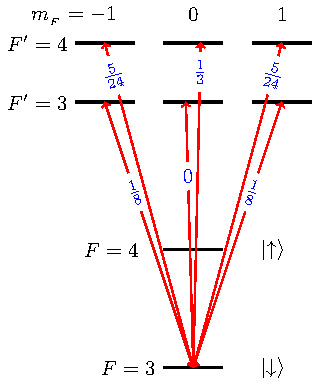
\includegraphics[scale=0.99]{./Figs/D1line_F3}}
\end{minipage}
\begin{minipage}{.49\linewidth}
\centering
\subfloat[]{\label{fig:D1line_F4}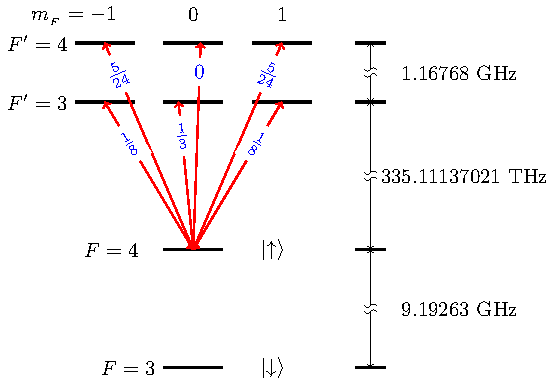
\includegraphics[scale=0.99]{./Figs/D1line_F4}}
\end{minipage}
\caption{Hyperfine level structure of the $ D_1 $ line transitions involving the clock states in $ 6S_{1/2} $ ground levels, their transition probabilities (numbers on the straight transition lines) and the two magic wavelength positions (wiggled lines). 
Subfig.~\ref{fig:D1line_F3} shows the transitions only involving the $ F=3,m=0 $ manifold. Subfig.~\ref{fig:D1line_F4} shows the transitions only involving the $ F=4,m=0 $ manifold.  }
\label{fig:D1line}
\end{figure}

Suppose there are $H$ and $V$ two orthogonal linear polarized mode components. The quantized forward-propagating electric field can be given by
\begin{align}
\hat{\mathbf{E}}^{(+)}(r\!_\perp,\phi,z) &= \sqrt{ \frac{2 \pi \hbar \omega_0}{ v_g \tau} } \big( \mathbf{u}_H(r\!_\perp,\phi) \hat{a}_H + \mathbf{u}_V(r\!_\perp,\phi) \hat{a}_V \big) e^{i \beta_0 z}.
\end{align}
The Hamiltonian due to the light-atom interaction can be written as
\begin{align}
H_{\rm eff}   &= -\hat{\mathbf{E}}^{(-)}(r^\prime\!\!_\perp,\phi',z')\cdot \tensor{\alpha}\cdot 
\hat{\mathbf{E}}^{(+)}(r^\prime\!\!_\perp,\phi',z') \label{eq:Heff_0}\\
 &=- \sum_{F,F'}\alpha_0(\Delta_{F,F'}) \left\{ C_{J'FF}^{(0)} \hat{\mathbf{E}}^{(-)} \cdot \hat{\mathbf{E}}^{(+)} \hat{\mathbbm{1}}_F \phantom{\frac{\hat{1}}{1}}\right. \nonumber\\
&\quad\quad\quad + i C_{J'FF'}^{(1)} \left(\hat{\mathbf{E}}^{(-)} \times \hat{\mathbf{E}}^{(+)} \right) \cdot \hat{ \mathbf{F}} \nonumber\\
&\quad\quad\quad  \left. + C_{J'FF}^{(2)} \hat{E}_i^{(-)} \hat{E}_j^{(+)} \left( \frac{ \hat{F}_i \hat{F}_j  + \hat{F}_j \hat{F}_i  }{2} - \frac{1}{3}\delta_{ij} \hat{ \mathbf{F}} \cdot \hat{\mathbf{F}}  \right) \right\}. 
\end{align}
\textcolor{blue}{Note: the effective Hamiltonian expressed in terms of Clebsch-Gordan coefficients in 
stead of the reduced coefficients is given in Appendix~\ref{sec:EffectiveHamiltonian_CG}. }

In the equation above, we have defined $ J $ as the total electric angular momentum quantum number, and the characteristic polarizability of the atom can be given by
\begin{align} \label{Eq::alpha0}
\alpha_0(\Delta) & =  -\frac{|  \bra{ J' }| d | \ket{ J } |^2}{\hbar \Delta } = - \frac{3 \lambda_{J' J}^3}{32 \pi^3} \frac{ \Gamma }{ \Delta }\quad \text{with}\quad 
\Gamma = \frac{1}{\hbar} \frac{4}{3} \frac{\omega_{J J'}^3}{c^3} | \bra{ J' }| d | \ket{ J } |^2.
\end{align}
In our case, the vector component of the atomic polarizability is zero. We can ignore the tensor component of the atomic polarizability in the far off-resonance regime. The scalar polarizability coefficient can be specified for our case as
\begin{align} \label{Eq::alpha0}
C_{J' F}^{(0)} &\equiv \sum_{F'} C_{J' F F'}^{(0)} =   \frac{2^{J'-1/2}}{3} =\left\{ \frac{1}{3},\frac{2}{3}\right\}.
\end{align}
The two values in the brackets are for the $D_1$ and $D_2$ lines, respectively.

The Hamiltonian can be further rewritten as
\begin{align}
H_{\rm eff} & = \frac{ \hbar }{ \tau}\Big( \chi_{H,\uparrow}\op{\uparrow}{\uparrow} +  \chi_{H,\downarrow} \op{\downarrow}{\downarrow} \Big) \hat{a}_H\dg \hat{a}_H \nonumber\\
&\quad +  \frac{ \hbar }{ \tau} \Big( \chi_{V,\uparrow}\op{\uparrow}{\uparrow} +  \chi_{V,\downarrow} \op{\downarrow}{\downarrow} \Big) \hat{a}_V\dg \hat{a}_V  ,
\end{align}
where the coupling strengths are defined as
\begin{align}
\chi_{H,\uparrow} &=  -\frac{2\pi\omega_0}{v_g} \mathbf{u}^*_{H}(r^\prime\!\!_\perp,\phi') \cdot\tensor{\alpha}_{\uparrow}\cdot \mathbf{u}_{H}(r^\prime\!\!_\perp,\phi') \\
\chi_{H,\downarrow} &=  -\frac{2\pi\omega_0}{v_g} \mathbf{u}^*_{H}(r^\prime\!\!_\perp,\phi') \cdot\tensor{\alpha}_{\downarrow}\cdot \mathbf{u}_{H}(r^\prime\!\!_\perp,\phi') \\
\chi_{V,\uparrow} &=  -\frac{2\pi\omega_0}{v_g}  \mathbf{u}^*_{V}(r^\prime\!\!_\perp,\phi') \cdot\tensor{\alpha}_{\uparrow}\cdot \mathbf{u}_{V}(r^\prime\!\!_\perp,\phi')  \\
\chi_{V,\downarrow} &=  -\frac{2\pi\omega_0}{v_g}  \mathbf{u}^*_{V}(r^\prime\!\!_\perp,\phi') \cdot\tensor{\alpha}_{\downarrow}\cdot \mathbf{u}_{V}(r^\prime\!\!_\perp,\phi'). 
\end{align}
with $\tensor{\alpha}_{\uparrow} \approx\sum_{F'=3,4}\frac{\alpha_0(\Delta_{4,F'})}{3}\mathbf{I}$
and $\tensor{\alpha}_{\downarrow} \approx\sum_{F'=3,4}\frac{\alpha_0(\Delta_{3,F'})}{3}\mathbf{I}$.
One can use different detuning regimes to detect the atomic clock state as a psuedo-spin state.

The coupling strength for the $ D_1 $ line probing can then be written as
\begin{align}
\chi_{H,\uparrow} &=  \sum_{F'} \frac{\chi_{H0}(F',4)}{3}, \quad
&\chi_{H,\downarrow} = \sum_{F'} \frac{\chi_{H0}(F',3) }{3}, \\
\chi_{V,\uparrow} &=  \sum_{F'} \frac{\chi_{V0}(F',4)}{3}, \quad
&\chi_{V,\downarrow} = \sum_{F'} \frac{\chi_{V0}(F',3) }{3} 
\end{align}
and 
\begin{align}
\chi_{H0}(F',F) &= \left( \frac{ \sigma_0}{A_{ef\!f}^H} \right) \left( \frac{\Gamma}{4 \Delta_{F,F'}} \right)=\frac{\Gamma_H^{1D}}{\Delta_{F,F'}},\quad
& A_{ef\!f}^H = \frac{1}{n_g|\mathbf{u}_{H}(r^\prime\!\!_\perp,\phi')|^2 },\\
\chi_{V0}(F',F) &= \left( \frac{ \sigma_0}{A_{ef\!f}^V} \right) \left( \frac{\Gamma}{4 \Delta_{F,F'}} \right)=\frac{\Gamma_V^{1D}}{\Delta_{F,F'}},\quad
& A_{ef\!f}^V = \frac{1}{n_g|\mathbf{u}^*_{V}(r^\prime\!\!_\perp,\phi')|^2 }.
\end{align}

The Hamiltonian can also be rewritten as below using the Stokes operators, $ \hat{S}_q $, and collective spin operators, $ \hat{J}_q $, with $ q=0,1,2,3 $.
\begin{align}
H_{\rm eff} 
=\frac{\hbar}{\tau} \Big\{ & \left[ \big( \chi_{H,\uparrow} + \chi_{H,\downarrow}\big) + \big(\chi_{V,\uparrow} + \chi_{V,\downarrow}\big) \right] \hat{J}_0 \hat{S}_0 \nonumber \\
+ & \left[ \big( \chi_{H, \uparrow} + \chi_{H,\downarrow}\big) - \big( \chi_{V,\uparrow} + \chi_{V,\downarrow} \big)\right]  \hat{J}_0 \hat{S}_1 \nonumber \\
+ & \left[ \big( \chi_{H,\uparrow} - \chi_{H,\downarrow}\big) + \big(\chi_{V,\uparrow} - \chi_{V,\downarrow} \big) \right] \hat{J}_3 \hat{S}_0 \nonumber \\
+ & \left[ \big( \chi_{H,\uparrow} - \chi_{H,\downarrow}\big) - \big(\chi_{V,\uparrow} - \chi_{V,\downarrow} \big) \right]  \hat{J}_3 \hat{S}_1\Big\}.
\end{align}
\missingfigure{Poincare sphere diagram with spin squeezing effect.}
The first term is an overall scalar shift and thus does not contribute to the relative dynamics.  The second term is a constant birefringence and can be canceled with a compensating waveplate as long as the atom number remains constant which is usually the case when the trapping time is fairly large compared to the measurement time. The first two terms can also be canceled when we have the detuning approximately equally biased for the $ F=3 $ and $ F=4 $ ground states. 
For example, we  can choose $ \Delta_3=-4.6 $ GHz and $ \Delta_4=4.6 $ GHz to the $ 6P_{1/2} $ excited state sublevels of cesium atoms to satisfy this condition, where the hyperfine splitting of the excited state can be ignored ($ ~500 $ MHz) compared to the detuning. However, we would like to leave the choice of detuning to control the third and fourth terms as will be discussed consequently. 

The final term describes the QND Faraday interaction we wish to isolate (similar to the Faraday interaction since we choose to use the $ y $-axis as the quantization axis), but this requires dealing with the third term that describes the effect of the scalar light shift on the rotation of the pseudo-spin.  Canceling the third term amounts to enforcing the condition that
\begin{align}
	\chi_{H,\uparrow} - \chi_{H,\downarrow} = \chi_{V,\downarrow} - \chi_{V,\uparrow} ,
\end{align}
which can be satisfied if we carefully choose the detuning of the probe light. The wavelength to choose to cancel the third term is atom position related, since the condition is determined by the effective mode areas which may have different ratios for the $ H $ and $ V $ modes at different locations. We can refer the exact wavelength to satisfy this condition as the \textit{magic wavelength}\index{magic wavelength}. If this condition can be met, then we can achieve an interaction of the form,
\begin{align}
	H_{\rm eff} = \frac{\hbar}{\tau} \chi_{\rm eff} \hat{J}_3 \hat{S}_1
\end{align}
where $\chi_{\rm eff} = 2(\chi_{H,\uparrow} - \chi_{H,\downarrow})$.  

Using this, we can prepare the spins in $ D $ state on the Bloch sphere and characterize the collective spin state along the $ z $-axis after the rotation along $ S_1 $ axis due to the photon-atom interaction. To achieve this, we use the $ \hat{S}_3 $ Stokes vector component measurement. As a result of the backaction of the polarization measurement, there is a squeezing to the collective spin state which results in a reduced uncertainty of measurement output. To see this, we assume the photon number, $N_L$, is large and apply the Holstein-Primakoff approximation to set $ \hat{S}_1=\sqrt{\frac{N_L}{2}}\hat{P}_L $ and $ \hat{S}_3=\sqrt{\frac{N_L}{2}}\hat{X}_L $, where $ \hat{X}_L$ and $\hat{P}_L $ are two photonic quadratures satisfying the commutation relationship that $ [\hat{X}_L,\hat{P}_L]=i $. Now the effective Hamiltonian can be written as
\begin{align}
H_{\rm eff} = \frac{\hbar}{\tau} \chi_{\rm eff} \sqrt{\frac{N_L}{2}}\hat{J}_3 \hat{P}_L. 
\end{align}
The $ \hat{S}_3 $ measurement is achieved through sending the signal light to one input port of a beam splitter along with a vacuum input on the other input port and then performing a balanced Homodyne measurement of the $ X_L $ quadrature. The equivalent Kraus operator conditional on this measurement can be defined by 
\begin{align}
\hat{A}_{X_L} &= \bra{X_L} e^{-i\chi_{\rm eff} \sqrt{\frac{N_L}{2}}\hat{J}_3 \hat{P}_L} \ket{0_L}\propto \exp\left\{ -\frac{\kappa T}{4}(l-\hat{J}_3)^2 \right\},
\end{align} 
where $ l=\frac{X_L}{\chi_{\rm eff} \sqrt{N_L/2}} $ is the measurement outcome in angular momentum units, and $ \kappa T=\chi_{\rm eff}^2N_L $ is the integrated measurement strength per spin. The shot noise resolution of the QND measurement is $ \sigma^2=\frac{1}{\kappa T} $. The Kraus operator $\hat{A}_{X_L}$ yields a backaction and generates a spin squeezing state\textcolor{blue}{[Reference]}. Given a spin coherent state (SCS) input with total spin quantum number $ J=N_A/2 $, the output state probability distribution can be given by 
\begin{align}
P_{L|l} \propto e^{-\frac{(L-\bar{L}(l))^2}{2\Delta J_{out}^2}},
\end{align}
where $ \Delta J_{out}^2 =\frac{\Delta J_{in}^2}{1+\xi}=\frac{J}{2(1+\xi)} $, $ \bar{L}(l)=\frac{l}{1+\xi} $, and $ \xi\equiv \frac{\Delta J_{in}^2}{\sigma^2}=\frac{J}{2\sigma^2}=\frac{\chi_{e\!f\!f}^2}{4}N_AN_L $ is the measurement strength which characterizes the measurement backaction and the squeezing effect. The ability to resolve the initial quantum variance of $ J_3 $ within the resolution of the meter is the key to QND squeezing.




\subsection{Birefringence and Faraday spectroscopies}

\textcolor{blue}{Discuss the homodyne detection and sensitivity to the atom number and operating frequency in the shot noise limit.  It relates to (i) the phase shift and (ii) the shot noise resolution of the polarimeter. Should cover expectation value and fluctuation measurements.}

For the birefringence measurement of the clock states discussed above, the fluctuation of the $ S_3 $ measurement is a combined effect of the shot noise fluctuation of the photon detector and the projection noise as the signal to determine the collective spin state. The square variance of the measurement is
\begin{align}
\Delta L^2 &= \Delta P^2_{SN} + \Delta P^2_S ,
\end{align}
where $ \Delta P^2_{SN} $ and $ \Delta P^2_{S} $ are the square variances of the shot noise and the signal, respectively. 
The smallest detectable spin polarization change from the input state is determined by the shot noise limit condition that 
\begin{align}
\Delta P_S = \Delta P_{SN},
\end{align}
where the standard variance of the signal can be estimated by
\begin{align}
\Delta P_S=P_0 \sin(\varphi_{_N}) \approx P_0 \varphi_{_N}
\end{align}
and the shot noise variance is determined by~\cite{Smith2003a}
\begin{align}
\Delta P_{SN} = \sqrt{\frac{P_0 \hbar \omega_0 }{2\eta \tau_{pd}}}.
\end{align}
Above, we have defined $P_0$ as the power of the input laser field, $\varphi_{_N}$ as the angle change 
of the output light on the Poincare sphere due to $N_A$ atoms, $\eta$ as the quantum efficiency of the 
photon detector, and $\tau_{pd}$ as the time constant of the detector. 

Using the magic wavelengths, we have 
\begin{align}
\chi_{\rm eff} (\omega) &= 2\left( \chi_{H,\uparrow} -\chi_{H,\downarrow} \right)\\
&= 2\sigma_0 n_g \sum_q |\mathbf{e}_q\cdot \mathbf{u}_H^*(r^\prime\!_\perp,\phi')|^2 \sum_{F'} 
\frac{\Gamma}{4} \left( \frac{|o^{J'F'}_{J4} C^{4 0;1q}_{F' q}|^2 }{\Delta_{4F'}+i\Gamma/2} - 
\frac{|o^{J'F'}_{J3} C^{3 0;1q}_{F' q}|^2 }{\Delta_{3F'}+i\Gamma/2}  \right),
\end{align}
or, in the dyadic Green function language from Equ.~\ref{eq:chiHGalpha}, 
\begin{align}
\chi_{\rm eff} (\omega)
&=  8\pi k_0^2 \tr \left\{ \mathrm{Im}\left[ 
\mathbf{G}^*_{HH}(\br^\prime\!_\perp,\br^\prime\!_\perp) \right] \cdot \left( 
\boldsymbol{\alpha}^{40;40} - \boldsymbol{\alpha}^{30;30} \right) 
\right\} . 
\end{align}
For the $ D_1 $ line transition, for example, there are two magic frequencies at $ \omega_3^m $ and $ \omega_4^m $ which close to the $ F=3 
\leftrightarrow F'=3 $ and $ F=4\leftrightarrow F'=4 $ transitions, respectively. In general, if we use the magic frequency, $ \omega_F^{\rm magic} $, which close to the $ F\leftrightarrow 
F'=F $ 
transition, we would have
\begin{align}
\chi_{\rm eff} (\omega_F^m) &= 8\pi k_0^2 \tr \left\{ \mathrm{Im}\left[ 
\mathbf{G}^*_{HH}(\br^\prime\!_\perp,\br^\prime\!_\perp) \right] \cdot \left( \boldsymbol{\alpha}^{40;40}(\omega_F^m) -   \boldsymbol{\alpha}^{30;30}(\omega_F^m) \right) 
\right\}\\
&= \sigma_0 n_g \frac{\Gamma}{2} \sum_q |\mathbf{e}_q\cdot 
\mathbf{u}_H^*(r^\prime\!_\perp,\phi')|^2 \sum_{F'} 
 \left( \frac{|o^{J'F'}_{J4} C^{4 0;1q}_{F' q}|^2 }{\Delta_{4F'}+i\Gamma/2} - 
 \frac{|o^{J'F'}_{J3} C^{3 0;1q}_{F' q}|^2 }{\Delta_{3F'}+i\Gamma/2}  \right),
\end{align}
The angle change on the Poincare sphere using the probe light at the magic frequency $ \omega_F^m $ can be given by
\begin{align}
\varphi_{_N} (\omega_F^m) &= N_A \left| \chi_{e\!f\!f} (\omega_F^m) \right| \\
&=   N_A \sigma_0 n_g\frac{\Gamma}{2} \sum_q |\mathbf{e}_q\cdot 
\mathbf{u}_H^*(r^\prime\!_\perp,\phi')|^2 
\sum_{F'}  \left( \frac{|o^{J'F'}_{J3} C^{3 0;1q}_{F' q}|^2 }{\Delta_{3F'} } - 
 \frac{|o^{J'F'}_{J4} C^{4 0;1q}_{F' q}|^2 }{\Delta_{4F'}}  \right).
\end{align} 
\textcolor{red}{We have ignored the decay rate whenever it is summed with the detuning terms.}

Now, we consider the critical case that $\eta =100\%$ and $\tau_{pd} = \frac{1}{\gamma_s}$, where the 
photon scattering rate
\begin{align}
\gamma_s &=\gamma_s (\omega_F)= \sum_{F,F'}\sigma(\Delta_{FF'}) \frac{I(\br')}{\hbar \omega_0}, 
%\approx \sum_{F'}\sigma(\Delta_{FF'}) \frac{I(\br')}{\hbar \omega_0}  , 
\end{align}
where $ I $ is the intensity of the light, and the photon scattering cross-section
\begin{align}
\sigma(\Delta_{FF'}) &=\frac{\sigma_0}{1+\frac{4\Delta^2_{FF'}}{\Gamma^2}}=\frac{\sigma_0\Gamma^2}{\Gamma^2+4\Delta^2_{FF'}} \mathbin{\color{red} \approx \sigma_0 
\frac{\Gamma^2}{4\Delta^2_{FF'}} \quad \text{(far detuning.)}}
\end{align}
Hence, by using the relationships given above, we can rewrite 
\begin{align}
\Delta P_{SN} (\omega_F^m) &=\frac{P_0\Gamma}{2}\sqrt{\frac{ \sigma_0 }{2A_{in}} \mathbin{\color{red}\sum_{F'} 
\left( \frac{1}{\Delta_{3F'}^2}+\frac{1}{\Delta_{4F'}^2}\right) }},\\
\Delta P_S (\omega_F^m) &= P_0  \varphi_{_N} (\omega_F^m) \nonumber\\
&\approx  P_0 N_A 
\sigma_0 n_g\frac{\Gamma}{2} 
\sum_q 
|\mathbf{e}_q\cdot 
\mathbf{u}_H^*(r^\prime\!_\perp,\phi')|^2 
\sum_{F'}  \left( \frac{|o^{J'F'}_{J3} C^{3 0;1q}_{F' q}|^2 }{\Delta_{3F'} } - 
 \frac{|o^{J'F'}_{J4} C^{4 0;1q}_{F' q}|^2 }{\Delta_{4F'}}  \right) \\
%&\approx  \frac{P_0 \Gamma}{2} N_A \sigma_0 n_g 
%\sum_q |\mathbf{e}_q\cdot \mathbf{u}_H^*(r^\prime\!_\perp,\phi')|^2 
%\sum_{F'} \frac{|o^{J'F'}_{JF} C^{F 0;1q}_{F' q}|^2 }{\Delta_{FF'}}  , 
\end{align}
with the effective mode areas
\begin{align}
A_{in } &= \frac{P_0}{I(\br')}=\frac{2}{| \mathbf{u}_H(r'_{\!\perp})|^2+ | 
\mathbf{u}_V(r'_{\!\perp})|^2}.
\end{align}
Therefore, the minimum detectable atom number, $ N_A^{min} $, can be obtained by forcing $ \Delta 
P_s = \Delta P_{SN} $ as
\begin{align}
N_A^{min}(\omega_F^m) &= \sqrt{\frac{A_{\rm eff}^2}{2A_{in}\sigma_0}} 
\end{align}
with the effective mode area defined as
\begin{align}
A_{\rm eff} &= \frac{ \sqrt{\sum_{F'}\left( \frac{1}{\Delta_{3F'}^2}+\frac{1}{\Delta_{4F'}^2}\right) }}{ n_g 
\sum_q |\mathbf{e}_q\cdot \mathbf{u}_H^*(r^\prime\!_\perp,\phi')|^2 
\sum_{F'}  \left( \frac{|o^{J'F'}_{J3} C^{3 0;1q}_{F' q}|^2 }{\Delta_{3F'} } - 
 \frac{|o^{J'F'}_{J4} C^{4 0;1q}_{F' q}|^2 }{\Delta_{4F'}}  \right) }.
\end{align}


\textcolor{blue}{Aside--only considering the scalar polarizability effect:} If we choose a detuning far-off 
the 
transition lines due to the hyperfine splitting 
of the excited states and ignore the tensor effect of the atomic polarizability, we will recover the 
simplified 
result given by Dawkins and coworkers~\cite{Dawkins2011}. 
The prove follows. Since the vector 
atomic polarizability vanish for the clock states, ignoring the tensor atomic polarizability means there is 
only scalar atomic polarizability left.
Therefore, the effective coupling strength can be given by 
\begin{align}
\chi_{e\!f\!f} &=[(\chi_{H,\uparrow}-\chi_{H,\downarrow})-(\chi_{V,\uparrow}-\chi_{V,\downarrow})]\\
&= 2C_{J'}^{(0)}(\Gamma_{H}^{1D}-\Gamma_V^{1D})\frac{1}{\Delta}
=\frac{C_{J'}^{(0)}\sigma_0\Gamma}{2}(\frac{1}{A^H_{e\!f\!f}}-\frac{1}{A^V_{e\!f\!f}})\frac{1}{\Delta},
\end{align} 
and the angle change by
\begin{align}
\varphi_{_N} &= N_A \chi_{e\!f\!f}\\
&=N_AC_{J'}^{(0)}n_g\sigma_0\frac{\Gamma}{2\Delta}\left[| \mathbf{u}_H(r'_{\!\perp})|^2- | 
\mathbf{u}_V(r'_{\!\perp})|^2 \right],
\end{align}
where $\frac{1}{\Delta}=\frac{1}{2}\sum_{F'}(\frac{1}{\Delta_{F',4}}-\frac{1}{\Delta_{F',3}})\approx \frac{1}{\Delta_{F',4}}$ and $ \sigma_0=3\lambda^2/2\pi $ is the resonant photon scattering cross-section of the atoms.

Now, we consider the critical case that $\eta =100\%$ and $\tau_{pd} = \frac{1}{\gamma_s}$, where the photon scattering rate
\begin{align}
\gamma_s &= \sigma(\Delta) \frac{I(\br')}{\hbar \omega_0}, 
\end{align}
where $ I $ is the intensity of the light, and the photon scattering cross-section
\begin{align}
\sigma(\Delta) &=\frac{\sigma_0}{1+\frac{4\Delta^2}{\Gamma^2}}\approx \sigma_0 
\frac{\Gamma^2}{4\Delta^2} \quad \text{(far detuning.)}
\end{align}
Hence, we can rewrite 
\begin{align}
\Delta P_{SN} &=P_0\sqrt{\frac{ \sigma_0 }{2A_{in}}}\frac{\Gamma}{2\Delta},\\
\Delta P_S &= N_A C_{j'}^{(0)}P_0 \frac{\sigma_0}{A_{e\!f\!f}}\frac{\Gamma}{2\Delta}, 
\end{align}
with the effective mode areas
\begin{align}
A_{in } &= \frac{P_0}{I(\br')}=\frac{2}{| \mathbf{u}_H(r'_{\!\perp})|^2+ | \mathbf{u}_V(r'_{\!\perp})|^2},\\
A_{e\!f\!f} &= \frac{1}{n_g\left[ | \mathbf{u}_H(r'_{\!\perp})|^2- | \mathbf{u}_V(r'_{\!\perp})|^2\right]}.
\end{align}
Therefore, the $ \Delta P_S = \Delta P_{SN}$ condition gives the resolution of the birefringence measurement in terms of the minimum atom number as
\begin{align}
N^{min}_A &= \frac{1}{C_{J'}^{(0)}}\sqrt{\frac{A_{e\!f\!f}^2}{A_{in}\sigma_0}}.
\end{align}

\missingfigure{Plots for $N^{min}_A$.}

\subsection{Other applications?} 


\section{Discussions}



\subsection{Connect to the Schrodinger picture?}
\textcolor{blue}{This has been done by Ben in one of his recent notes. }



%\subsection{Group velocity}

\subsection{Achievable phase shift with scalar atomic polarizabilities?}
\todo[inline]{To be deleted for this paper.}
\textcolor{blue}{Show the phase shift and the decay rate are results of the combination effect of the free dipole radiation and the reflection from the nanofiber interface. Discuss the phase shift control landscape and the difference with the vacuum case. Apply to a phase gate.}
\begin{align}
\delta\phi &= -\frac{\Gamma^{1D}_\mu}{2\Delta},\\
\frac{\Gamma^{1D}_\mu}{\Gamma_0} &= \frac{6\pi c}{\omega}\frac{\sum_g\mathbf{d}_{eg}\cdot \mathrm{Im}\left[\mathbf{G}_g^\mu(\br',\br') \right]\cdot\mathbf{d}_{eg}^* }{\sum_g|\mathbf{d}_{eg}|^2} = 1+ \frac{3}{2} \frac{\mathrm{Im}\left[\sum_g\mathbf{d}_{eg}^*\cdot \mathbf{E}^{(R,\mu)}_g(\br') \right]}{\sum_g|\mathbf{d}_{eg}|^2 k^3}\nonumber\\
&=\frac{3\pi}{2}\left(\frac{c}{\omega}\right)^2\frac{c}{v_g} \frac{\sum_{g}|\mathbf{d}_{eg}\cdot \mathbf{u}^\mu(\br')|^2}{\sum_g|\mathbf{d}_{eg}|^2}\\
\mathbf{E}^{(R,\mu)}_g(\br') &= -\frac{1}{4\pi k^2} \mathbf{G}^{(R,\mu)}_g(\br',\br')\cdot \mathbf{d}_{eg}.
\end{align}
The index $ R $ indicates the component of reflection, and $\mu=(\beta,m,f)  $ identifies the normalized fiber mode $ \mathbf{u}^\mu(\br') $. 

We can write 
\begin{align}
\Gamma_{vac} &= \frac{4\omega_0^3|\mathbf{d}|^2}{3\hbar c^3}=-\frac{8\pi \omega_0^2}{\hbar c^2}\left[ \mathbf{d}\cdot \mathrm{Im}[\mathbin{\color{red}{\mathbf{G}^{(0)}}}(\br',\br')]\cdot \mathbf{d}^* \right]\\
\Gamma &= -\frac{8\pi \omega_0^2}{\hbar c^2}\left[ \mathbf{d}\cdot \mathrm{Im}[\mathbf{G}(\br',\br')]\cdot \mathbf{d}^* \right]=-\frac{8\pi \omega_0^2}{\hbar c^2}\left[ \mathbf{d}\cdot \mathrm{Im}[\mathbin{\color{red}{\mathbf{G}^{(0)}}}(\br',\br')+\mathbin{\color{red}{\mathbf{G}^{(R)}}}(\br'\br')]\cdot \mathbf{d}^* \right]\\
\end{align}
The decay rate is a result of the superposition of the free dipole radiation and the reflection from the nanofiber interface.

\begin{align}
\Gamma &\propto -\mathbf{d}\cdot \mathrm{Im}[\mathbf{G}(\br',\br')]\cdot \mathbf{d}^* \\
&=\mathrm{tr}\left[ \mathbin{\color{red}{(\mathbf{d}^*\mathbf{d})}}\cdot\mathbin{\color{blue}{ \mathrm{Im}[\mathbf{G}^*(\br',\br')]}}  \right]\\
&= \mathrm{tr}\left[ \boldsymbol{\rho} \cdot \mathrm{Im}[\mathbf{G}^{*}(\br',\br')]  \right]\ge 0
\end{align}
where $\boldsymbol{\rho}=(\mathbf{d}^*\mathbf{d})$ is defined as the dipole orientation tensor which is merely a property of the atoms. The dyadic Green function part is only a property of the waveguide.  

By mathematical definition, $\mathrm{Im}[\mathbf{G}^{*}(\br',\br')]$ is positive definite. 
\begin{align}
\mathrm{Im}[\mathbf{G}^{*}(\br',\br')] &= \sum_{i=1,2,3} \mathbin{\color{red}{g_i}}\hat{\mathbf{v}}_i\hat{\mathbf{v}}_i,\,\text{with}\, g_i>0.
\end{align}
$\hat{\mathbf{v}}_i$ form the principal axes of the decay rate. The principal axes indicate the dipole orientations along which the interference between the free dipole radiation and the reflected field (equivalent to the radiation from the image dipole) is most constructive and destructive.   
\begin{align}
\Gamma &= C(\omega)\sum_i g_i(\hat{\mathbf{v}}_i\cdot \boldsymbol{\rho}\cdot \hat{\mathbf{v}}_i) 
= \sum_i \mathbin{\color{blue}{(d'_i)^2}} \mathbin{\color{red}{g_i}} \\
&= \mathbin{\color{red}{\Gamma_1}}\cos^2\phi\sin^2\theta+\mathbin{\color{red}{\Gamma_2}}\sin^2\phi\sin^2\theta+\mathbin{\color{red}{\Gamma_3}}\cos^2\theta,
\end{align}
where $ d'_i=\sqrt{\hat{\mathbf{v}}_i\cdot \boldsymbol{\rho}\cdot \hat{\mathbf{v}}_i}$ and $\mathbf{d}'=\sum_i d'_i\hat{\mathbf{v}}_i$ defines the equivalent dipole orientation of the atomic polarizability transition.

The range of decay rates:
$$\mathbin{\color{red}{\Gamma_1}}=\Gamma_{max}\mathbin{\color{red}{\ge \Gamma (\theta,\phi) \ge}} \Gamma_{min}=\mathbin{\color{red}{\Gamma_3}}$$

Quantum transitions and dipole orientations correspondence:
\begin{align}
\sigma_+ &\leftrightarrow \mathbf{d}_+\propto \frac{1}{\sqrt{2}}(i\mathbf{e}_{r\!_\perp}+\mathbf{e}_\phi)\\
\pi &\leftrightarrow \mathbf{d}_0 \propto \mathbf{e}_z\\
\sigma_- &\leftrightarrow \mathbf{d}_-\propto \frac{1}{\sqrt{2}}(-i\mathbf{e}_{r\!_\perp}+\mathbf{e}_\phi).
\end{align}
Example: completely mixed state decay rate calculation:
\begin{align}
\boldsymbol{\rho} &=\frac{1}{3}(\boldsymbol{\rho}_++\boldsymbol{\rho}_0+\boldsymbol{\rho}_-)=\frac{d_0^2}{3}\boldsymbol{I}\\
\Gamma &=\frac{C(\omega)}{3}d_0^2 \mathrm{tr}\left[ \mathrm{Im}[\mathbf{G}^*(\br',\br')] \right]=\frac{1}{3}(\Gamma_1+\Gamma_2+\Gamma_3).
\end{align}
This is equivalent to assume the dipole is uniformly pointing to any direction, and hence
$\Gamma = \int \frac{\mathrm{\Omega}}{4\pi}\Gamma(\theta,\phi)=\frac{1}{3}(\Gamma_1+\Gamma_2+\Gamma_3)$.

\missingfigure{Some plots for emission surfaces here.}

The phase shift is proportional to the time integral of the path on the emission rate surface. The range of the decay rates determines the achievable phase shift in a unit time. However, the emission rate surface for the vacuum case is a uniform sphere and the corresponding phase shift in a given time is a constant independent from the orientation of the dipole with a scalar atomic polarizability. Therefore, it is possible to use the scalar atomic polarizability to realize a wide controllable phase shift range in the off-resonance regime that the vacuum configuration can hardly achieve. 


\subsection{Interference due to a one-sided or two-sided atom chain}\label{sec:atomchain}
\textcolor{blue}{Effect of an infinite long one-side chain... S matrix, reflectivity... Random filling effect...}

\textcolor{blue}{To include many-atom interference effect, we can use the linear optical transformation matrix formalism. The transformation of modes should be the same for both Green function and Heisenberg picture approaches. Here, I am using the semiclassical Green function results first, and then the Heisenberg picture results. } 


From Equ.~\eqref{eq:Cmf} and the results above, one can generalize the field transformation relationship due to the presence of an atom and an arbitrary incident mode $\mathbf{u}_{m'f'}(\br)$ with mode amplitude $E_{m'f'}$ to give
\begin{align}
\mathbf{E}^{out}(\br) &= \sum_{mf}E_{mf}\mathbf{u}_{m'f'}(\br),\\
E_{mf} &= \left[\delta_{mm'}\delta_{ff'}+C_{m'f'}^{mf}\right]E_{m'f'},
\end{align}
with 
\begin{align}
C^{mf}_{m'f'}
&= i2\pi k_0 n_g\alpha  {\mathbf{u}^{mf}}^*(r'_{\!\perp})\cdot \mathbf{u}_{m'f'}(r'_{\!\perp})e^{i\beta_0 
(f'-f)z'+i(m'-m)\phi'}.\label{eq:Cmfmf}
\end{align}
Therefore, one can define the scattering matrix $\mathbf{S}\equiv \left\{S^{mf}_{m'f'}|\,m,f,m',f'=\pm 1 \right\}$ with elements $S^{mf}_{m'f'}=\delta_{mm'}\delta_{ff'}+C_{m'f'}^{mf}$. 

Notice that, $\br'=(r\!_\perp^\prime,\phi',z')$ indicates where the atom is sitting. If there are many atoms which are sitting at one transverse plane with the same $z'$ position, one should sum over all those atom indexes to obtain the total scattering matrix at a $z$-slice. In our case, the atoms can sit at some random positions of either $\phi'=0$ or $\phi'=\pi$ two sides of a periodic chain. For simplicity, we always use $z=z'=0$ for the scattering matrix $\mathbf{S}(\phi')$ calculation on one $z$-slice. We define the free propagating transformation matrix, $\mathbf{P}(\Lambda)\equiv \left\{P^{mf}_{m'f'}(\Lambda)|\,m,f,m',f'=\pm 1 \right\}$, by
\begin{align}
P^{mf}_{m'f'}(\Lambda) &= \delta_{mm'}\delta_{ff'}e^{if\beta_0 \Lambda},
\end{align}
where $\Lambda$ is the minimum distance or geometric period between atoms along the propagating direction of the guided light. The total field amplitude after the interaction with the last atom along the nanofiber due to the random occupied two-side chain of atoms can be given by
\begin{align}
\left( E_{mf}^{out}\right) &= [\eta_{N,+} \mathbf{S}(0) +\eta_{N,-}\mathbf{S}(\pi) +(1-\eta_{N,+})(1-\eta_{N,-})\eye] \mathbf{P}(\Lambda)\nonumber\\
&\quad [\eta_{N-1,+} \mathbf{S}(0) +\eta_{N-1,-}\mathbf{S}(\pi)+(1-\eta_{N-1,+})(1-\eta_{N-1,-})\eye ] \mathbf{P}(\Lambda)\nonumber\\
&\quad \ldots [\eta_{2,+} \mathbf{S}(0) +\eta_{2,-}\mathbf{S}(\pi)+(1-\eta_{2,+})(1-\eta_{2,-})\eye ] \mathbf{P}(\Lambda)\nonumber\\
&\quad [\eta_{1,+} \mathbf{S}(0) +\eta_{1,-}\mathbf{S}(\pi) +(1-\eta_{1,+})(1-\eta_{1,-})\eye] \left( E_{m'f'}^{in}\right)\\
&= \left\{ \prod_{i=N}^2 [\eta_{i,+} \mathbf{S}(0) +\eta_{i,-}\mathbf{S}(\pi)+(1-\eta_{i,+})(1-\eta_{i,-})\eye ] \mathbf{P}(\Lambda)\right\} \nonumber\\
&\quad [\eta_{1,+} \mathbf{S}(0) +\eta_{1,-}\mathbf{S}(\pi)+(1-\eta_{1,+})(1-\eta_{1,-})\eye ]\left( E_{m'f'}^{in}\right)\\
&= \left\{ \prod_{i=N}^2 \mathbf{S}_i \mathbf{P}(\Lambda)\right\} \mathbf{S}_1 \left( E_{m'f'}^{in}\right),\label{eq:transE}
\end{align}
where $\mathbf{S}_i=\eta_{i,+} \mathbf{S}(0) +\eta_{i,-}\mathbf{S}(\pi)+(1-\eta_{i,+})(1-\eta_{i,-})\eye $ denote the scattering matrix due to the randomly occupied atoms at the $i^{\mathrm{th}}$ $z$-slice with random occupation variables $\eta_{i,\pm}=0$ or $1$ on both sides of the atom chain. The distribution of the random variables $\eta_{i,\pm}$ reflects how the atom chain is occupied. 

For the case that both sides ($ \phi'=0 $ and $\pi  $) of the atom chain are fully occupied along the $z$-direction, the scattering matrix elements can be given by
\begin{align}
\!\!\!\!\!\!S^{mf}_{m'f'} &= 2\delta_{mm'}\delta_{ff'} + i2\pi k_0 n_g\alpha  
{\mathbf{u}_{mf}}^*(r'_{\!\perp})\cdot \mathbf{u}_{m'f'}(r'_{\!\perp})[1+e^{i(m'-m)\pi}]\\
&= 2\delta_{mm'}\delta_{ff'} + i2\pi k_0 n_g\alpha  \left[ |u_{r\!_\perp}(r'_{\!\perp})|^2+mm' 
|u_\phi(r'_{\!\perp})|^2+ff'|u_z(r'_\perp)|^2\right][1+e^{i(m'-m)\pi}]\\
&= 2\delta_{mm'}\delta_{ff'} + i4\pi k_0 n_g\alpha  \left[ |u_{r\!_\perp}(r'_{\!\perp})|^2+mm' 
|u_\phi(r'_{\!\perp})|^2+ff'|u_z(r'_\perp)|^2\right].
\end{align}
We have treated the atomic polarizability as a scalar and used Born approximation here. Notice that, the polarization-dependent factor $[1+e^{i(m'-m)\pi}]$ always yields $2$ with $m,m'=\pm 1$ for the $\mathrm{HE}_{11}$ guided modes. If there are high-order guided modes, we expect to see destructive Birefringence effects for modes with odd modal index gaps. 

This can also be understood by looking into the equations derived in the Heisenberg picture. The equivalent scattering matrix elements due to an atom positioned at $\br'=(r'_\perp,\phi',z'=0)$ can be obtained by making $t\rightarrow t_0$ from Equ.~\eqref{eq:Smfmft}:
\begin{align}\label{eq:Smfmfphi_Heisenberg}
S^{mf}_{m'f'}(\phi') &=\delta_{mm'}\delta_{ff'}-i\frac{2\pi 
g_\mu^*(\omega)g_{\mu'}(\omega)}{\Delta+i\Gamma/2}\\
&= \delta_{mm'}\delta_{ff'}-i\frac{ \frac{2\pi 
\omega}{v_g}\mathbf{u}^*_{mf}(\br'_\perp)\cdot\mathbf{d}_{ge} 
\mathbf{d}_{eg}\cdot\mathbf{u}_{m'f'}(\br'_\perp)e^{i(f'-f)\beta_0 z'}}{\Delta+i\Gamma/2}\\
&=  \delta_{mm'}\delta_{ff'}-i\frac{ \frac{2\pi 
\omega}{v_g}\mathbf{u}^*_{mf}(r'_\perp)\cdot\mathbf{d}_{ge} 
\mathbf{d}_{eg}\cdot\mathbf{u}_{m'f'}(r'_\perp)e^{i(m'-m)\phi'}}{\Delta+i\Gamma/2}.
\end{align}
Therefore, the total scattering transformation matrix for the atom pair on both sides of the $x$-axis can be given by
\begin{align}\label{eq:Smfmf2_Heisenberg}
S^{mf}_{m'f'}(\phi') &=S^{mf}_{m'f'}(\phi'=0)+S^{mf}_{m'f'}(\phi'=\pi)\\
&=  2\delta_{mm'}\delta_{ff'}-i\frac{ \frac{4\pi 
\omega}{v_g}\mathbf{u}^*_{mf}(r'_\perp)\cdot\mathbf{d}_{ge} 
\mathbf{d}_{eg}\cdot\mathbf{u}_{m'f'}(r'_\perp)}{\Delta+i\Gamma/2}\\
&= 2\delta_{mm'}\delta_{ff'}-i 4\pi k_0 
n_g\mathbf{u}^*_{mf}(r'_\perp)\cdot\boldsymbol{\alpha}\cdot\mathbf{u}_{m'f'}(r'_\perp) .
\end{align}

When $\beta_0 L$ is a multiple of $\pi$, the free propagation transformation matrix is proportional to a unitary matrix, and hence can be extracted out from the total transformation matrix formula (Equ.~\eqref{eq:transE}). In that case, the total phase shift for a given input mode can be treated as the sum of the phase shift due to each individual atoms on both sides of the $z$-slices. Otherwise, there will be the asymmetric effect on the phase shifts of the forwarding and backwarding modes. Moreover, under the framework derived above, if we can ignore the backward propagating modes--which is approximately true if it is far from satisfying the geometric Bragg condition that $ \beta_0\Lambda=n\pi $, the free propagating transformation matrix $\mathbf{P}(\Lambda)$ is also proportional to a unitary matrix, and hence the total phase shifts for individual forwarding modes can still be treated as a sum over all slices of atoms along the propagating direction. Physically, the asymmetric mixing of forward and backward propagating modes may be the major barrier to treat the total phase shift as the sum over all individual elements.  

\todo[inline]{Energy is not conserving under the Born approximation. How does the radiation power distribute after every event of scattering? A better model to explain what we should observe for the Birefringence effect.}

\section{Conclusions}

\begin{acknowledgments}
X.Q. would like to particularly thank Ninnat Dangniam, Tzu-Cheng Wu and Matthew Chase for their inspiring discussions. We thank the UNM Center for Advanced Research Computing for computational resources used in this work.
\end{acknowledgments}

\appendix
\section{Radiation fields from an atom close to a nanofiber}\label{app:fieldcalculation}
As discussed in section~\ref{sec:GFmethod}, the 9 elements of a dyadic electric Green function is proportional to the local electric field components due to the radiation from an electric dipole orientated in some basis directions. The spontaneous radiation field components can be calculated through decomposing the field into reflected and transmitted field components and matching up the boundary conditions of the nanofiber which can be treated as an infinitely long cylindrical dielectric medium. The detailed calculations have been conducted by Nha, Klimov and others in their earlier publications~\cite{Nha1997,Klimov2004}. We summarize some of those results in this section. 

One can separate the electric and magnetic fields into free-dipole radiation, reflected and transmitted parts. For example, the electric field can be written as 
\begin{align}
\boldsymbol{\mathcal{E}}(\br) &= \boldsymbol{\mathcal{E}}^{(0)}(\br) + 
\boldsymbol{\mathcal{E}}^{(R)}(\br)+\boldsymbol{\mathcal{E}}^{(T)}(\br)\\
&=
	\begin{cases}
	  \boldsymbol{\mathcal{E}}^{(0)} (\br)+ \boldsymbol{\mathcal{E}}^{(R)}(\br), & r\!_\perp > a,\\
	  \boldsymbol{\mathcal{E}}^{(T)}(\br), & r\!_\perp\leq a.
	\end{cases} \label{Etotalfiber}
\end{align}
where the superscripts $0$, $R$ and $T$ indicate the free-dipole radiation, reflection and transmission components of the field, and $ a $ is the radius of the nanofiber. For a translationally invariant waveguide, which means the index of refraction of the waveguide is independent of the propagating axis $z$, the electric and magnetic fields can be written as 
\begin{align}
\bmc{E}(\br) &= \bmc{E}(\br\!_\perp)\exp(i\beta z), & \bmc{H}(\br) &= \bmc{H}(\br\!_\perp)\exp(i\beta 
z),
\end{align}
where $ \beta $ is the propagation constant and $ \br\!_\perp $ is the position vector in the transverse 
plane perpendicular to the $ z $-axis. We let the index of refraction of the nanofiber be
\begin{align}
n=n(r\!_\perp)&=\begin{cases}
	  n_2=1, & r\!_\perp > a,\\
	  n_1, & r\!_\perp\leq a.
	\end{cases} \label{nfiber}
\end{align}
To find the fields, we need to calculate the longitudinal components (the $z$-components) of the fields, and the transverse components can be obtained through $z$-components using the following relationships:
\begin{subequations}\label{EHzgauss}
\begin{align}
\mathcal{E}_{r\!_\perp} &= \frac{i}{\kappa_i^2} \left[ \beta \pp{\mathcal{E}_z }{r\!_\perp} + 
  \frac{k}{r\!_\perp} 
\pp{\mathcal{H}_z}{\phi} \right]= \frac{i\beta}{\kappa_i^2} \pp{\mathcal{E}_z }{r\!_\perp} - 
  \frac{km}{r\!_\perp \kappa_i^2} {\mathcal{H}_z}, \\
\mathcal{E}_\phi &= \frac{i}{\kappa_i^2} \left[\frac{\beta}{r\!_\perp} 
\pp{\mathcal{E}_z}{\phi} - k 
\pp{\mathcal{H}_z}{r\!_\perp} 
\right] = -\frac{\beta m}{r\!_\perp \kappa_i^2} 
{\mathcal{E}_z} - \frac{ik}{\kappa_i^2} 
\pp{\mathcal{H}_z}{r\!_\perp},\\
\mathcal{H}_{r\!_\perp} &= \frac{i}{\kappa_i^2} \left[ \beta \pp{\mathcal{H}_z}{r\!_\perp} 
- \frac{kn^2}{r\!_\perp}\pp{\mathcal{E}_z}{\phi} \right]= \frac{i\beta}{\kappa_i^2} \pp{\mathcal{H}_z}{r\!_\perp} 
+ \frac{kn^2m}{r\!_\perp \kappa_i^2} {\mathcal{E}_z},\\
\mathcal{H}_\phi &= \frac{i}{\kappa_i^2} \left[ \frac{\beta}{r\!_\perp} \pp{\mathcal{H}_z}{\phi} + 
 kn^2 \pp{\mathcal{E}_z}{r\!_\perp} \right] = -\frac{\beta m}{r\!_\perp \kappa_i^2} {\mathcal{H}_z} + 
  \frac{ikn^2}{\kappa_i^2} \pp{\mathcal{E}_z}{r\!_\perp}
\end{align}
\end{subequations}
with $ \kappa_i=\kappa_1 $ or $ \kappa_2 $ and $ n=n_1 $ or $ n_2 $ for the corresponding space region. 
We use Gauss units in this paper, and assume the material of the nanofiber is non-magnetic, and hence $ 
\boldsymbol{\mathcal{B}}= \mu_r\boldsymbol{\mathcal{H}}\approx \boldsymbol{\mathcal{H}} $ with the relative permeability $ \mu_r\approx 1 $. We have also defined the transverse propagation constant inside of the nanofiber, $ \kappa_1 $, by $\kappa_1^2=n_1^2k-\beta^2$. Similarly, one can define the transverse propagation constant outside of the nanofiber, $ \kappa_2 $, by $ \kappa_2^2=n_2^2k-\beta^2=k^2-\beta^2 $.

The longitudinal components of the electrical and magnetic fields can be expanded as Fourier transformations over the $ \beta $ space,
\begin{subequations}\label{ET0Rexpand}
\begin{align}
\mathcal{E}^{(T)}_z
&= \sum_{m=-\infty}^\infty \int \mathrm{d}\beta e^{im(\phi-\phi') + i\beta (z-z')} c_{m\beta} J_m (\kappa_1r\!_\perp),\\
\mathcal{E}^{(0)}_{z} &= \sum_{m=-\infty}^\infty \int \mathrm{d}\beta e^{im(\phi-\phi') + i\beta (z-z')} \mathcal{E}^{(0)}_{z,m\beta}(r\!_\perp)\\
\mathcal{E}^{(R)}_z 
&= \sum_{m=-\infty}^\infty \int \mathrm{d}\beta e^{im(\phi-\phi') + i\beta (z-z')} a_{m\beta} H_m^{(1)} (\kappa_2r\!_\perp),
\end{align}
\end{subequations}
\begin{subequations}\label{BT0Rexpand}
\begin{align}
\mathcal{B}^{(T)}_z 
&= \sum_{m=-\infty}^\infty \int \mathrm{d}\beta e^{im(\phi-\phi') + i\beta (z-z')} d_{m\beta} J_m (\kappa_1r\!_\perp),\\
% + E_{m\beta} Y_m(hr\!_\perp)\right],\\
\mathcal{B}^{(0)}_{z} &= \sum_{m=-\infty}^\infty \int \mathrm{d}\beta e^{im(\phi-\phi') + i\beta (z-z')} \mathcal{B}^{(0)}_{z,m\beta}(r\!_\perp)\\
\mathcal{B}^{(R)}_z 
&= \sum_{m=-\infty}^\infty \int \mathrm{d}\beta e^{im(\phi-\phi') + i\beta (z-z')} b_{m\beta} H_m^{(1)} (\kappa_2r\!_\perp),
\end{align}
\end{subequations}
in which $J$ and $H$ indicate the first kind of the Bessel function and the Hankel function as the cylindrical harmonics; the atom is positioned at $\br'=(r^\prime\!_\perp,\phi',z')$ with an electric dipole moment $\mathbf{d}_0=(d^0_{r\!_\perp}, d^0_\phi,d^0_z)$ in the atom's coordinate system. In the fiber's coordinate system, the dipole moment observed at an arbitrary position $\br$ is defined by the three components defined below:
\begin{align}
d_{r\!_\perp}\! &= \cos(\phi\!-\!\phi')d^0_{r\!_\perp}\!\!+\!\sin(\phi\!-\!\phi')d^0_\phi=\frac{1}{\sqrt{2}}\left(-e^{-i(\phi\!-\!\phi')}d_++e^{i(\phi\!-\!\phi')}d_- \right),\\
d_\phi &=\cos(\phi\!-\!\phi')d^0_\phi\!-\!\sin(\phi\!-\!\phi')d^0_{r\!_\perp}=\frac{i}{\sqrt{2}}\left(e^{-i(\phi\!-\!\phi')}d_++e^{i(\phi\!-\!\phi')}d_- \right),\\
d_z &= d^0_z,
\end{align}
where we have defined the position-independent reduced dipole components
\begin{align}
d_\pm \equiv \mp \frac{1}{\sqrt{2}}(d^0_{r\!_\perp}\pm id^0_{\phi}).
\end{align}
The terms associated with $d_\pm$ in the dipole moment formula lower or raise the mode index or the angular momentum quantum number, $m$, of the interacting fiber modes by $1$. Notice that we have used $\phi\!-\!\phi'$ as the projected angle between $\mathbf{r}$ and $\mathbf{r}'$ on the transverse plane to make the relationship valid in general. In most of our calculations, we usually position the atom on the $x$-axis of the fiber coordinate and set $z'=0$.


The free radiation field components associated with the $ e^{im(\phi-\phi')+i\beta (z-z')} $ term (the $m$-th mode components) for the $r\!_\perp<r'\!_\perp$ region can be given by
\begin{align}
\mathcal{B}_{z,m\beta}^{(0)} &= \frac{ik\kappa_2}{2\sqrt{2}}J_m(pr\!_\perp)\left[ d_{+} H_{m+1}^{(1)}(\kappa_2r'\!\!_\perp) \!-\! d_- H_{m-1}^{(1)}(\kappa_2r'\!_\perp) \right],\\
\mathcal{B}_{\phi,m\beta}^{(0)} &= \frac{ik}{2}\left[ \frac{\beta d_{-}}{\sqrt{2}} J_{m-1}\left( \kappa_2r\!_\perp \right)H_{m-1}^{(1)}\left( {\kappa_2r\!_\perp^{\prime} }\right) -\frac{\beta d_+}{\sqrt{2}} J_{m+1}\left( \kappa_2r\!_\perp \right)H_{m+1}^{(1)}\left( {\kappa_2r\!_\perp^{\prime} }\right)\right. \nonumber\\ 
&\qquad\quad \left. + \frac{i\kappa_2d^0_z}{2}\left(J_{m-1}(\kappa_2r\!_\perp)-J_{m+1}(\kappa_2r\!_\perp) \right)H_m^{(1)}(\kappa_2r\!_\perp^{\prime}) \right],\\
\mathcal{B}_{r\!_\perp, m\beta}^{(0)} &= \frac{k}{2}\left[\frac{i m d^0_z}{r\!_\perp} J_m\left( \kappa_2r\!_\perp \right) H_m^{(1)}\left( {\kappa_2r\!_\perp^{\prime} }\right) \right. \nonumber\\
&\qquad \left. +\frac{\beta d_+}{\sqrt{2}} J_{m\!+\!1}(\kappa_2r\!_\perp) H_{m\!+\! 1}^{(1)}(\kappa_2r\!_\perp^{\prime}) \!+\! \frac{\beta d_-}{\sqrt{2}} J_{m\!-\! 1}(\kappa_2r\!_\perp)H_{m\!-\!1}^{(1)}(\kappa_2r\!_\perp^{\prime})   \right],\\
\mathcal{E}_{z,m\beta}^{(0)} 
&= \frac{\kappa_2}{2}J_{m}\left( \kappa_2r\!_\perp \right)\left[  id^0_z \kappa_2 H_m^{(1)}\left( {\kappa_2r\!_\perp^{\prime} }\right) \phantom{\frac{d^0_z}{\sqrt{2}}} \right. \nonumber\\
&\qquad\qquad\qquad \left. + \frac{\beta d_{+}}{\sqrt{2}} H_{m+1}^{(1)}\left( {\kappa_2r\!_\perp^{\prime} }\right) +\frac{\beta d_-}{\sqrt{2}} H_{m-1}^{(1)}\left( {\kappa_2r\!_\perp^{\prime} }\right) \right], \\
\mathcal{E}_{\phi,m\beta}^{(0)} 
&= -\frac{im\beta d^0_z}{2r\!_\perp} J_{m}\left( \kappa_2r\!_\perp \right) H_m^{(1)}\left( {\kappa_2r\!_\perp^{\prime} }\right) \nonumber\\
&\quad+\frac{d_+}{2\sqrt{2}} \left[ \frac{m\kappa_2}{r\!_\perp}J_{m}\left( \kappa_2r\!_\perp \right)-k^2 J_{m+1}\left( \kappa_2r\!_\perp \right)\right] H_{m+1}^{(1)}\left( {\kappa_2r\!_\perp^{\prime} }\right) \nonumber\\
&\quad+ \frac{d_-}{2\sqrt{2}}\left[\frac{m\kappa_2}{r\!_\perp}J_m\!\left( \kappa_2r_\perp \right)-k^2J_{m-1}\!\left( \kappa_2r_\perp \right) \right] H_{m-1}^{(1)}\!\left( {\kappa_2r\!_\perp^{\prime} }\right),\\
\mathcal{E}_{r\!_\perp,m\beta}^{(0)} 
&= \frac{\beta \kappa_2d^0_z}{4}\left[ J_{m+1}\!\left( \kappa_2r\!_\perp \right)-J_{m-1}\!\left( \kappa_2r_\perp \right)\right] H_m^{(1)}\left( {\kappa_2r\!_\perp^{\prime} }\right)\nonumber\\ 
&\quad -\frac{d_+}{2\sqrt{2}}\left[ i\beta^2J_{m+1}\!\left( \kappa_2r_\perp \right) +\frac{im\kappa_2}{r\!_\perp}J_m\!\left( \kappa_2r_\perp \right)\right] H_{m+1}^{(1)}\!\left( {\kappa_2r\!_\perp^{\prime} }\right)\nonumber\\
&\quad + \frac{d_-}{2\sqrt{2}}\left[ i\beta^2J_{m-1}\!\left( \kappa_2r_\perp \right) +\frac{im\kappa_2}{r\!_\perp}J_m\!\left( \kappa_2r_\perp \right)\right] H_{m-1}^{(1)}\!\left( {\kappa_2r\!_\perp^{\prime} }\right).
\end{align}
The magnetic and electrical fields components for $ r\!_\perp>r'\!_\perp $ are 
\begin{align}
\mathcal{B}_{z,m\beta}^{(0)} &= \frac{ik\kappa_2}{2\sqrt{2}}H^{(1)}_m(\kappa_2r\!_\perp)\left[ d_{+} J_{m+1}(\kappa_2r'\!\!_\perp) \!-\! d_- J_{m-1}(\kappa_2r'\!_\perp) \right],\\
\mathcal{B}_{\phi,m\beta}^{(0)} &= \frac{ik}{2}\left[ \frac{\beta d_{-}}{\sqrt{2}} H^{(1)}_{m-1}\left( \kappa_2r\!_\perp \right)J_{m-1}\left( {\kappa_2r\!_\perp^{\prime} }\right) -\frac{\beta d_+}{\sqrt{2}} H^{(1)}_{m+1}\left( \kappa_2r\!_\perp \right)J_{m+1}\left( {\kappa_2r\!_\perp^{\prime} }\right)\right. \nonumber\\ 
&\qquad\quad \left. + \frac{i\kappa_2d^0_z}{2}\left(H^{(1)}_{m-1}(\kappa_2r\!_\perp)-H^{(1)}_{m+1}(\kappa_2r\!_\perp) \right)J_m(\kappa_2r\!_\perp^{\prime}) \right],\\
\mathcal{B}_{r\!_\perp, m\beta}^{(0)} &= \frac{k}{2}\left[\frac{i m d^0_z}{r\!_\perp} H^{(1)}_m\left( \kappa_2r\!_\perp \right) J_m\left( {\kappa_2r\!_\perp^{\prime} }\right) \right. \nonumber\\
&\qquad \left. +\frac{\beta d_+}{\sqrt{2}} H^{(1)}_{m\!+\!1}(\kappa_2r\!_\perp) J_{m\!+\! 1}(\kappa_2r\!_\perp^{\prime}) \!+\! \frac{\beta d_-}{\sqrt{2}} H^{(1)}_{m\!-\! 1}(\kappa_2r\!_\perp) J_{m\!-\!1}(\kappa_2r\!_\perp^{\prime})   \right],\\
\mathcal{E}_{z,m\beta}^{(0)} 
&= \frac{\kappa_2}{2}H^{(1)}_{m}\left( \kappa_2r\!_\perp \right)\left[  id^0_z \kappa_2 J_m\left( {\kappa_2r\!_\perp^{\prime} }\right) \phantom{\frac{d^0_z}{\sqrt{2}}} \right. \nonumber\\
&\qquad\qquad\qquad \left. + \frac{\beta d_{+}}{\sqrt{2}} J_{m+1}\left( {\kappa_2r\!_\perp^{\prime} }\right) +\frac{\beta d_-}{\sqrt{2}} J_{m-1}\left( {\kappa_2r\!_\perp^{\prime} }\right) \right], \\
\mathcal{E}_{\phi,m\beta}^{(0)} 
&= -\frac{im\beta d^0_z}{2r\!_\perp} H^{(1)}_{m}\left( \kappa_2r\!_\perp \right) J_m\left( {\kappa_2r\!_\perp^{\prime} }\right) \nonumber\\
&\quad+\frac{d_+}{2\sqrt{2}} \left[ \frac{m\kappa_2}{r\!_\perp}H^{(1)}_{m}\left( \kappa_2r\!_\perp \right)-k^2 H^{(1)}_{m+1}\left( \kappa_2r\!_\perp \right)\right] J_{m+1}\left( {\kappa_2r\!_\perp^{\prime} }\right) \nonumber\\
&\quad+ \frac{d_-}{2\sqrt{2}}\left[\frac{m\kappa_2}{r\!_\perp}H^{(1)}_m\!\left( \kappa_2r_\perp \right)-k^2 H^{(1)}_{m-1}\!\left( \kappa_2r_\perp \right) \right] J_{m-1}\!\left( {\kappa_2r\!_\perp^{\prime} }\right),\\
\mathcal{E}_{r\!_\perp,m\beta}^{(0)} 
&= \frac{\beta \kappa_2d^0_z}{4}\left[ H^{(1)}_{m+1}\!\left( \kappa_2r\!_\perp \right)-H^{(1)}_{m-1}\!\left( \kappa_2r_\perp \right)\right] J_m\left( {\kappa_2r\!_\perp^{\prime} }\right)\nonumber\\ 
&\quad -\frac{d_+}{2\sqrt{2}}\left[ i\beta^2H^{(1)}_{m+1}\!\left( \kappa_2r_\perp \right) +\frac{im\kappa_2}{r\!_\perp}H^{(1)}_m\!\left( \kappa_2r_\perp \right)\right] J_{m+1}\!\left( {\kappa_2r\!_\perp^{\prime} }\right)\nonumber\\
&\quad + \frac{d_-}{2\sqrt{2}}\left[ i\beta^2H^{(1)}_{m-1}\!\left( \kappa_2r_\perp \right) +\frac{im\kappa_2}{r\!_\perp}H^{(1)}_m\!\left( \kappa_2r_\perp \right)\right] J_{m-1}\!\left( {\kappa_2r\!_\perp^{\prime} }\right).
\end{align}

By using the boundary conditions at $ r\!_\perp=a $ and Equ.~\eqref{Etotalfiber} that
\begin{align}
%\varepsilon_f \mathcal{E}_{r\!_\perp}(r\!_\perp =a^> ) = \mathcal{E}_{r\!_\perp}(r\!_\perp =a^< ),\\
\mathcal{E}_{z}(r\!_\perp =a^> ) = \mathcal{E}_{z}(r\!_\perp =a^< ),\\
%\mathcal{B}_{r\!_\perp}(r\!_\perp =a^> ) = \mathcal{B}_{r\!_\perp}(r\!_\perp =a^< ),\\
\mathcal{B}_{z}(r\!_\perp =a^> ) = \mathcal{B}_{z}(r\!_\perp =a^< ),\\
\mathcal{E}_{\phi}(r\!_\perp =a^> ) = \mathcal{E}_{\phi}(r\!_\perp =a^< ),\\
\mathcal{B}_{\phi}(r\!_\perp =a^> ) = \mathcal{B}_{\phi}(r\!_\perp =a^< ),
\end{align}
where $ a^< $ and $ a^> $ denote the boundaries at the sides less and larger than $ a $, and the connections between field components (Equ.~\eqref{EHzgauss}), we can obtain all unknown coefficients. To summarize, we have~\cite{Klimov2004}
\begin{align}
a_{m\beta} &= \frac{na}{P^2+QR},\\
b_{m\beta} &= \frac{nb}{P^2+QR},\\
c_{m\beta} &= \frac{\mathcal{E}_{z,m\beta}^{(0)}(r\!_\perp\!=\!a)+ H_m^{(1)}(\kappa_2a)a_{m\beta}}{J_m(\kappa_1a)},\\
d_{m\beta} &= \frac{\mathcal{H}_{z,m\beta}^{(0)}(r\!_\perp\!=\!a)+ H_m^{(1)}(\kappa_2a)b_{m\beta}}{J_m(\kappa_1a)},
\end{align}
where
\begin{align}
na &= \kappa_1^2\kappa_2^2aJ_m(\kappa_1a)PE_{\phi,m\beta}^{(0)}(r\!_\perp\!=\!a) \nonumber\\
&\quad + \kappa_2^2\left[J_m(\kappa_1a)\beta mP+kan_1^2\kappa_1 \dd{}{(\kappa_1a)}J_m(\kappa_1a)Q \right] E_{z,m\beta}^{(0)} \nonumber\\
&\quad + i\kappa_1^2\kappa_2^2 aJ_m(\kappa_1a)QB_{\phi,m\beta}^{(0)}(r\!_\perp\!\!=\!a) \!-\! im\beta \kappa_1\kappa_2J_m(\kappa_1a)SB_{z,m\beta}^{(0)}(r\!_\perp\!\!=\!a),\\
nb &= \kappa_1^2\kappa_2^2aJ_m(\kappa_1a)PB_{\phi,m\beta}^{(0)}(r\!_\perp\!=\!a) \nonumber\\
&\quad + \kappa_2^2\left[J_m(\kappa_1a)\beta mP-ka\kappa_1 \dd{}{(\kappa_1a)}J_m(\kappa_1a)R \right] B_{z,m\beta}^{(0)} \nonumber\\
&\quad + i\kappa_1^2\kappa_2^2 aJ_m(\kappa_1a)RE_{\phi,m\beta}^{(0)}(r\!_\perp\!\!=\!a) \!+\! im\beta \kappa_1\kappa_2J_m(\kappa_1a)TE_{z,m\beta}^{(0)}(r\!_\perp\!\!=\!a),
\end{align} 
and
\begin{align}
P &=m\beta k^2J_m(\kappa_1a)H_m^{(1)}(\kappa_2a)(n_1^2-1),\\
Q &=-\kappa_1\kappa_2ak\left[ \kappa_1J_m(\kappa_1a)\dd{}{(\kappa_2a)}H_m^{(1)}(\kappa_2a)-\kappa_2H_m^{(1)}(\kappa_2a)\dd{}{(\kappa_1a)}J_m(\kappa_1a) \right],\\
R &=\kappa_1\kappa_2ak\left[ \kappa_1J_m(\kappa_1a)\dd{}{(\kappa_2a)}H_m^{(1)}(\kappa_2a)-\kappa_2n_1^2H_m^{(1)}(\kappa_2a)\dd{}{(\kappa_1a)}J_m(\kappa_1a) \right],\\
S &=\kappa_1\kappa_2ak\left[ \kappa_2J_m(\kappa_1a)\dd{}{(\kappa_2a)}H_m^{(1)}(\kappa_2a)-\kappa_1H_m^{(1)}(\kappa_2a)\dd{}{(\kappa_1a)}J_m(\kappa_1a) \right],\\
T &=\kappa_1\kappa_2ak\left[ \kappa_2J_m(\kappa_1a)\dd{}{(\kappa_2a)}H_m^{(1)}(\kappa_2a)-\kappa_1n_1^2H_m^{(1)}(\kappa_2a)\dd{}{(\kappa_1a)}J_m(\kappa_1a) \right].
\end{align}

The integral in Equs.~\eqref{EHzgauss} should be chosen along path $C_1$ as shown in Fig.~\ref{fig:integralpath} to detour the branch cuts and singularities of integrands. The branch cuts are determined by $ \mathrm{Im}[\kappa_2],\mathrm{Im}[\kappa_1]>0 $ to ensure the integrands single-valued and remain on the Riemann sheet where the radiation fields decrease at the infinities. Note that there are only two branch cuts along the $ y $-axis and within $ [-n_2k,n_2k] $ on the $ x $-axis originated from $ \mathrm{Im}[\kappa_2]=0 $. The $ \mathrm{Im}[\kappa_1]=0 $ condition does not yield any other new branch cuts where the integrands discontinue. Approximately, we use dashed lines to indicate the branch cuts on the left subplots in Fig.~\ref{fig:integralpath}. There are also poles on the complex plane of $ \beta $, and are located at $ \pm\beta_0 $ characterizing the guided modes ($\mathrm{HE}_{11}$ modes for the single-mode nanofiber). We exclude the singularities by closing the integration contours on the upper-half complex plane of $ \beta $ when $ z>0 $ and the lower-half plane when $ z<0 $ to ensure the Fourier transform convergent at infinities. Since the closed contour integrals vanish, the integrals along $ C_1 $ can be transformed to the contour integrals detouring the branch cuts and around the poles which correspond to the radiation mode and the guided mode components, respectively. We have used the fact that the integrands vanish at infinities (red solid contour paths). Along the contour paths, we choose $ \kappa_1 $ always positive real while $ \kappa_2 $ being negative real in the first and third quadrants and being positive real in the second and forth quadrants. 

\begin{figure}
\begin{minipage}{.91\linewidth}
\centering
\subfloat[]{\label{contourplot_upper}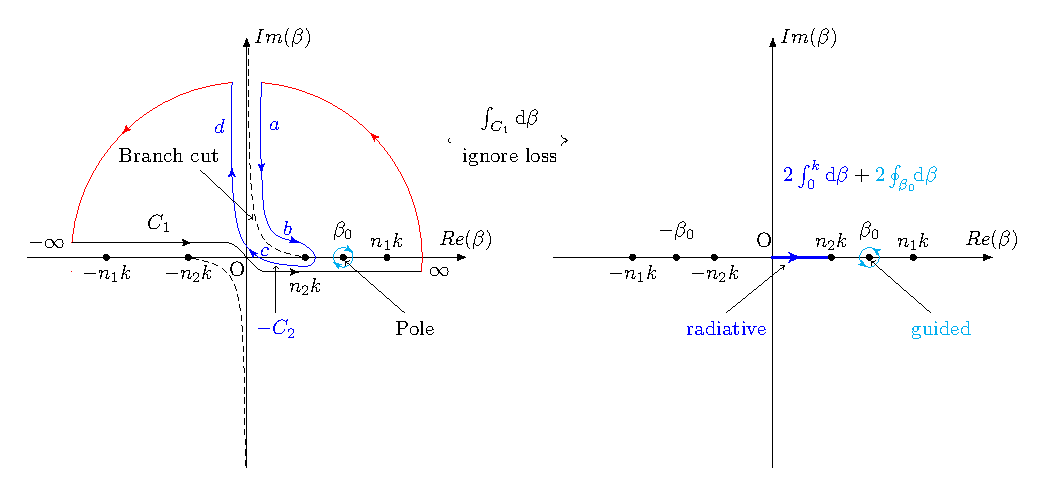
\includegraphics[scale=0.75]{./Figs/contourplot_upper}}
\end{minipage}
\par\medskip
\begin{minipage}{.91\linewidth}
\centering
\subfloat[]{\label{contourplot_lower}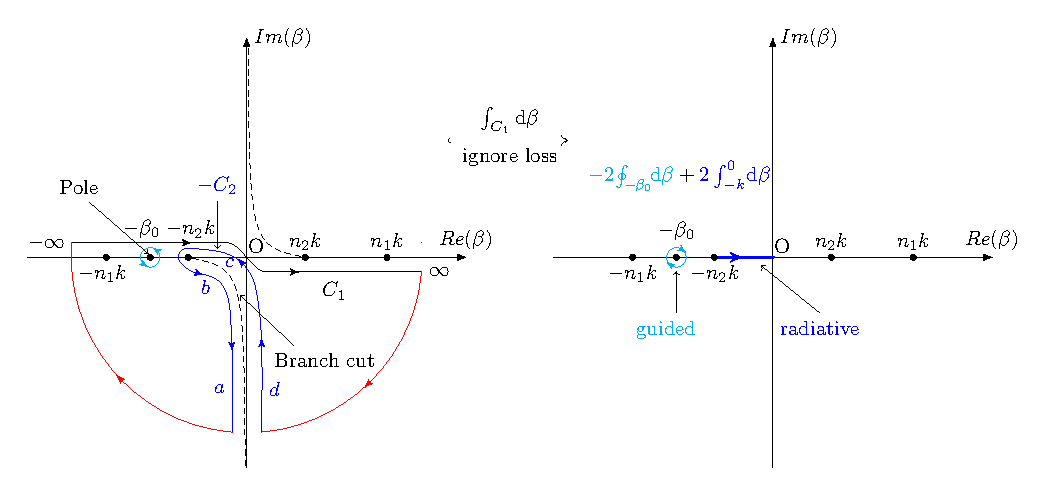
\includegraphics[scale=0.75]{./Figs/contourplot_lower}}
\end{minipage}
\caption{Equivalent integration paths to calculate the radiation and guided fields. For $ z>0 $, we can use the zero-valued contour integral path drawn in subfig.~\ref{contourplot_upper} to calculate the integration along path $ C_1 $. The simplified integration path by ignoring waveguide losses is given in the top-right plot. It only contains the forward propagating mode contributions with radiation and guided mode components as divided through the real-axis integral and the residual of the pole. For the $ z<0 $ case, the contour integral analysis is given in subfig.~\ref{contourplot_lower}, which only includes the backward propagating mode contributions.}
\label{fig:integralpath}
\end{figure}

\textcolor{blue}{More information: Physics meaning of the sections detouring the branch cuts and poles...} The integrals along the vertical sections of the contour paths, $ a $ and $ d $, cancel. The integrals along the horizontal sections, $ b $ and $ c $, double one the other. In the end, the contour integral detouring the branch cuts yields $ 2\int_0^k\mathrm{d}\beta $ for $ z>0 $ or $ 2\int_{-k}^0\mathrm{d}\beta $ for $ z<0 $ with $ n_2=1 $. Similarly, one can show that the contour integrals around the poles with separated segments of positive and negative real $ \kappa_2 $'s are equivalent to $ \pm 2\oint_{\pm \beta_0}\!\!\mathrm{d}\beta $ with positive real $ \kappa_2 $. When $ z=0 $, the full integral along path $ C_1 $ can be rewritten as the average value of the $ z>0 $ and $ z<0 $ limits. Therefore, we have 
\begin{align}
\int_{C_1}\mathrm{d}\beta =\int_{-k}^k\mathrm{d}\beta +\oint_{\beta_0}\mathrm{d}\beta -\oint_{-\beta_0}\!\!\mathrm{d}\beta,
\end{align}
where the first integral yield the radiation mode contribution and the last two terms yield the guided mode contribution in two respective propagation directions. When we calculate the decay rates or phase shift due to the presence of atoms along a nanofiber, we can use this decomposition relationship of integrals. Notice that, the guided mode contribution part should only include the $ m=\pm 1 $ $\mathrm{HE}_{11}$ modes when summing over mode index $ m $ for a single-mode nanofiber. 



\section{Group index of refraction and mode functions of the fundamental guided modes}\label{ch:guidedmodes}
The longitudinal propagation constant $\beta_0$ of the fundamental $\mathrm{HE}_{11}$ guided mode is the solution of $\beta$ determined by the fiber eigenvalue equation~\cite{LeKien2005}
\begin{align}
f(\kappa_1,q,k,\beta) &=0,
\end{align}
where
\begin{align}
f(\kappa_1,q,k,\beta) &=\frac{J_0(\kappa_1a)}{\kappa_1aJ_1(\kappa_1a)}+\frac{n_1^2+n_2^2}{2n_1^2}\frac{K_1^\prime(qa)}{qaK_1(qa)}-\frac{1}{\kappa_1^2a^2} \\
&+\left\{\left[\frac{n_1^2-n_2^2}{2n_1^2}\frac{K_1^\prime(qa)}{qaK_1(qa)} \right]^2 +\frac{\beta^2}{n_1^2k^2}\left(\frac{1}{q^2a^2}+\frac{1}{\kappa_1^2a^2} \right)^2 \right\}^{1/2}
\end{align}
and the transverse propagation constants $\kappa_1=\sqrt{n_1^2k^2-\beta^2}$ and $q=\sqrt{\beta^2-n_2^2k^2}=\sqrt{\beta^2-k^2}$. $J_n$ and $K_n$ stand for the Bessel functions of the first kind and the modified Bessel functions of the second kind, respectively. 

We differentiate the fiber eigenvalue equation above with respect to $ \beta $ on both sides, and obtain
\begin{align}
\dd{f}{\beta} &= \pp{f}{\kappa_1} \left(\pp{\kappa_1}{k}\dd{k}{\beta}+\pp{\kappa_1}{\beta} \right) + \pp{f}{q}\left(\pp{q}{k}\dd{k}{\beta}+\pp{q}{\beta} \right) +\pp{f}{k}\dd{k}{\beta}+\pp{f}{\beta}=0
\end{align}
Therefore, the group index of refraction of the fundamental modes of the nanofiber can be given by
\begin{align}
 n_g &= \dd{\beta}{k} = -\frac{\pp{f}{\kappa_1}\pp{\kappa_1}{k}+\pp{f}{q}\pp{q}{k}+\pp{f}{k}}
{\pp{f}{\kappa_1}\pp{\kappa_1}{\beta}+\pp{f}{q}\pp{q}{\beta}+\pp{f}{\beta}}.
\end{align}

\missingfigure{Frequency stability, linearity and maybe other aspects of the group index of refraction.}

The fundamental mode functions, $\mathbf{u}^{(\mu)}(r\!_\perp,\phi,z)$, of the electric components of the fiber~\cite{LeKien2005,Lacroute2012} can be separated into $r\!_\perp-$, $\phi-$ and $z-$dependent parts, and are characterized by the mode index $\mu=(\beta_0,f,\xi)$, where $f=\pm 1$ indicates forward and backward propagating directions and $\xi $ indicates the polarization state of the mode. For a quasicircularly polarized fundamental mode, we use $\xi=m=\pm $ to indicate the counterclockwise and clockwise rotations, respectively; for a quasilinearly polarized fundamental mode, we usually use $\xi=\phi_0$ to indicate the rotation angle, $\phi_0$, of the polarization axis from the $x$-axis; specially, we use $\xi=H$ or $V$ when the quasilinear polarization axis is along the $x$-axis or $y$-axis, respectively. For the circularly polarized case, the fundamental mode can be written as 
\begin{align}
\mathbf{u}^{(\mu)}(r\!_\perp,\phi,z) &=u^{(\mu)}_{r\!_\perp}(r\!_\perp) e^{if\beta_0 z+im\phi }\hat{r}\!_\perp +u^{(\mu)}_{\phi}(r\!_\perp) e^{if\beta_0 z+im\phi } \hat{\phi} +u^{(\mu)}_{z}(r\!_\perp)e^{if\beta_0 z+im\phi }\hat{z}\\
&=u_{r\!_\perp}(r\!_\perp) e^{if\beta_0 z+im\phi }\hat{r}\!_\perp + m u_{\phi}(r\!_\perp) e^{if\beta_0 z+im\phi }\hat{\phi} + f u_z (r\!_\perp) e^{if\beta_0 z+im\phi }\hat{z},
\end{align}
where the forwarding, counterclockwise rotating guided mode components, $\mathbf{u}(r\!_\perp)$, are determined, for $r\!_\perp<a$, by
\begin{subequations}
\label{urtcrla}
\begin{align}
u_{r\!_\perp}(r\!_\perp) &=-A\frac{\beta_0}{2\kappa_1} \left[ (1-s)J_0(\kappa_1r\!_\perp)-(1+s)J_2(\kappa_1r\!_\perp) \right]\\
u_\phi(r\!_\perp) &=  -imA \frac{\beta_0}{2\kappa_1} \left[ (1-s)J_0(\kappa_1r\!_\perp) +(1+s)J_2(\kappa_1r\!_\perp) \right] \\
u_z(r\!_\perp) &= ifA J_1(\kappa_1r\!_\perp),
\end{align}
\end{subequations}
and, for $ r_\perp>a $, by
\begin{subequations}
\label{urtcrga}
\begin{align}
u_{r\!_\perp}(r\!_\perp) &=-A\frac{\beta_0}{2\kappa_1}\frac{J_1(\kappa_1a)}{K_1(qa)} \left[ (1-s)K_0(qr\!_\perp)+(1+s)K_2(qr\!_\perp) \right]\\
u_\phi(r\!_\perp) &=  -imA \frac{\beta_0}{2\kappa_1} \frac{J_1(\kappa_1a)}{K_1(qa)} \left[ (1-s)K_0(qr\!_\perp) - (1+s)K_2(qr\!_\perp) \right] \\
u_z(r\!_\perp) &= ifA \frac{J_1(\kappa_1a)}{K_1(qa)} K_1(qr\!_\perp),
\end{align}
\end{subequations}
with
\begin{align}
s &= \left[\frac{1}{(\kappa_1a)^2}+ \frac{1}{(qa)^2} \right] \left[ \frac{J_1'(\kappa_1a)}{\kappa_1aJ_1(\kappa_1a)} + \frac{K'_1(qa)}{qaK_1(qa)} \right],\\
\kappa_1 &= \sqrt{k^2 n_1^2-\beta_0^2}.
\end{align}
The normalization factor, $A$, is determined by the normalized energy that 
\begin{align}
1 &= \int_0^{2\pi} \!\!\mathrm{d} \phi \int_0^\infty\!\!\mathrm{d}r\!_\perp r\!_\perp\,  n^2(\br\!_\perp)|\boldsymbol{\mathcal{E}}^g(\br\!_\perp)|^2 = 2\pi A^2 a^2 (n_1^2P_1 + n_2^2P_2),
\end{align}
where the stored energy distribution factors are
\begin{align}
\!\!\!\!\! P_1
&= \frac{\beta_0^2}{4\kappa_1^2}\!\left\{(1\!-\! s)^2\!\left[J_0^2(\kappa_1a)\!+\! J_1^2(\kappa_1a) \right] \!+\!(1\!+\!s)^2\!\left[J_2^2(\kappa_1a)\!-\!J_1(\kappa_1a)J_3(\kappa_1a) \right]\right\}\nonumber\\
&\quad +\frac{1}{2}\left[J_1^2(\kappa_1a)-J_0(\kappa_1a)J_2(\kappa_1a) \right] \\
\!\!\!\!\! P_2
&= \frac{\beta_0^2J_1^2(\kappa_1a)}{4q^2K_1^2(qa)}\!\left\{\phantom{\frac{1}{1}}\!\!\!\!(1\!-\!s)^2\!\left[K_1^2(qa)\!-\!K_0^2(qa) \right]\right.\nonumber\\
&\quad\left. \!+(1\!+\!s)^2\!\!\left[K\!_1\!(qa)K\!_3\!(qa)\!-\! K_2^2\!(qa) \right]\!+\!\frac{2q^2}{\beta^2}\!\!\left[K\!_0\!(qa)K\!_2\!(qa)\!-\!K_1^2\!(qa) \right]  \right\}.
\end{align}
Using this basis, the electric part of a guided field with quasicircularly propagating mode index $\mu=(\beta_0, f, m)$ can be written as 
\begin{align}
E^{(\mu)}(r\!_\perp,\phi,z,t) &=E_0\left[u_{r\!_\perp}\!(r\!_\perp) \hat{r}\!_\perp \!+\! m u_{\phi}(r\!_\perp) \hat{\phi} \!+\! f u_z (r\!_\perp) \hat{z}\right]e^{if\beta_0 z+im\phi-i\omega t }.
\end{align}
The power propagating inside and outside the fiber can be given in terms of the time averaged Poynting vector along the propagation direction, $\left< S_z \right>$, by
\begin{align}
P_{in} &= \int_0^{2\pi} \mathrm{d}\phi \int_0^a \left< S_z \right> r\!_\perp \mathrm{d}r\!_\perp\\
P_{out} &= \int_0^{2\pi} \mathrm{d}\phi \int_a^\infty \left< S_z \right> r\!_\perp \mathrm{d}r\!_\perp.
\end{align}
The total power $ P=P_{in}+P_{out} $. One can show that the normalization constant $ E_0 A $ reads
\begin{align}\label{eq:EA}
E_0 A=\sqrt{\frac{4\mu_0\omega P}{\pi a^2 \beta_0}}\left(D_{in} + D_{out} \right)^{-1/2},
\end{align}
where
\begin{align}
D_{in} &= (1-s)\left[ 1+(1-s)\frac{\beta_0^2}{\kappa_1^2}\right] \left(J_0^2(\kappa_1a) + J_1^2(\kappa_1a) \right) \nonumber\\
&\quad + (1+s)\left[ 1+(1+s)\frac{\beta_0^2}{\kappa_1^2}\right] \left(J_2^2(\kappa_1a)- J_1(\kappa_1a)J_3(\kappa_1a) \right)\\
D_{out} &= \frac{J_1^2(\kappa_1a)}{K_1^2(qa)}\left\{ (1-s)\left[ 1-(1-s)\frac{\beta_0^2}{q^2}\right] \left(K_0^2(qa) - K_1^2(qa) \right)\right. \nonumber\\
&\quad \left. + (1\!+\! s)\left[ 1\!-\! (1\!+\! s)\frac{\beta_0^2}{q^2}\right] \left(K_2^2(qa)\! -\! K_1(qa)K_3(qa) \right) \right\}.
\end{align}



For a quasilinearly polarized fundamental guided mode, the electric part of the mode can be written as 
\begin{align}
\mathbf{u}^{(\beta_0, f, \phi_0)}(r\!_\perp,\phi,z) &= \frac{1}{\sqrt{2}} \left(\mathbf{u}^{(\beta_0, f, +)}(r\!_\perp,\phi,z)e^{-i\phi_0} +\mathbf{u}^{(\beta_0, f, -)}(r\!_\perp,\phi,z)e^{i\phi_0} \right)\\
&= \sqrt{2}\left[u_{r\!_\perp}(r\!_\perp)\cos(\phi-\phi_0)\hat{\mathbf{r}}\!_\perp + iu_\phi(r\!_\perp)\sin(\phi-\phi_0)\hat{\boldsymbol{\phi}} \right. \nonumber \\
&\quad\quad \left. + fu_z(r\!_\perp)\cos(\phi-\phi_0)\hat{\mathbf{z}} \right]e^{if\beta_0 z}.
\end{align}
One can write down an arbitrary quasilinearly polarized electric field in the form similar to the quasicircularly polarized case with $E_0A$ satisfying the same relationship defined in Equ.~\eqref{eq:EA}. 

Particularly, when $\phi_0=0$ and $\pi/2$, we obtain the $H$ and $V$ fundamental modes as
\begin{align}
\mathbf{u}^{(\beta_0, f, H)}(r\!_\perp,\phi,z)
&= \sqrt{2}\left[u_{r\!_\perp}(r\!_\perp)\cos(\phi)\hat{\mathbf{r}}\!_\perp + iu_\phi(r\!_\perp)\sin(\phi)\hat{\boldsymbol{\phi}} + fu_z(r\!_\perp)\cos(\phi)\hat{\mathbf{z}} \right]e^{if\beta_0 z}\\
\mathbf{u}^{(\beta_0, f, V)}(r\!_\perp,\phi,z)
&= \sqrt{2}\left[u_{r\!_\perp}(r\!_\perp)\sin(\phi)\hat{\mathbf{r}}\!_\perp - iu_\phi(r\!_\perp)\cos(\phi)\hat{\boldsymbol{\phi}}  + fu_z(r\!_\perp)\sin(\phi)\hat{\mathbf{z}} \right]e^{if\beta_0 z}.
\end{align}

\todo[inline]{To show $v_g=\frac{P}{W}$ using the formulas above?}

\section{Light-atom interaction in the dispersive regime}\label{sec:lightatominteract}
\textcolor{blue}{Detailed derivation can be found in Qi's hand-written notes on \textit{Dispersive field-atom interaction Hamiltonian}. The special case of a single mode propagating in a homogeneous medium can be found in Ben's dissertation (chapter 4). }


The dispersive light shift interaction describes an atom's effective response to an electric field when the excited states can be adiabatically eliminated from the quantum dynamics.  This reduced description applies when the saturation parameter of atoms is much smaller than 1:
\begin{align} \label{Eq::SatParameter}
	s = \frac{ \Omega^2/4}{\Delta^2 + \Gamma^2/4} \ll 1,  
\end{align}
where $\Omega$ is the Rabi frequency, $\Gamma$ is the total spontaneous emission rate of the atoms, and $\Delta = \omega_0 - \omega_{eg}$ is the probe detuning from the atomic resonance frequency $\omega_{eg}$ of the given excited and ground states. As the saturation parameter is proportional to the ratio of the Rabi frequency to the detuning, $\Omega/\Delta$, physically this allows condition \erf{Eq::SatParameter} to be satisfied even for large driving power (Rabi frequency) as long as the probe laser is far enough detuned.  In this limit, the atom-light coupling can be described by the dispersive light-shift interaction,
\begin{align} 
	\hat{H}_{\rm eff} & = \sum_{f,f'=\pm 1}\hat{H}_{\rm eff}^{ff'} =- \sum_{f,f'=\pm 1}\hat{\mathbf{E}}^{(-)}_f(\mathbf{r}' ) \cdot \tensor{\alpha} \cdot \hat{\mathbf{E}}^{(+)}_{f'}(\mathbf{r}' )\\
	&= - \hat{\mathbf{E}}^{(-)}_+(\mathbf{r}' ) \cdot \tensor{\alpha} \cdot \hat{\mathbf{E}}^{(+)}_+(\mathbf{r}' )
	- \hat{\mathbf{E}}^{(-)}_+(\mathbf{r}' ) \cdot \tensor{\alpha} \cdot \hat{\mathbf{E}}^{(+)}_-(\mathbf{r}' )\nonumber\\
	&\quad - \hat{\mathbf{E}}^{(-)}_-(\mathbf{r}' ) \cdot \tensor{\alpha} \cdot \hat{\mathbf{E}}^{(+)}_+(\mathbf{r}' )
	- \hat{\mathbf{E}}^{(-)}_-(\mathbf{r}' ) \cdot \tensor{\alpha} \cdot \hat{\mathbf{E}}^{(+)}_-(\mathbf{r}' ), \label{Eq::LightShiftHam}
\end{align}
where the electric field operator is evaluated at the atomic position $\mathbf{r}'$, and the electric component of the guided field can be given by
\begin{align}
\hat{\mathbf{E}} &= (\hat{\mathbf{E}}^{(+)}e^{-i\omega_0 t}+c.c.)/2
\end{align}   
with
\begin{align}
\hat{\mathbf{E}}^{(+)}(\br) &= \sum_{f=\pm 1} \hat{\mathbf{E}}^{(+)}_f(\br) = \sqrt{\frac{2\pi \hbar \omega_0}{v_g\tau}}\sum_{f=\pm 1} \left[ \mathbf{u}_{Hf}(\br\!_\perp)\hat{a}_{Hf} + \mathbf{u}_{Vf}(\br\!_\perp)\hat{a}_{Vf} \right]e^{if\beta_0 z},
\end{align}
where $\mathbf{u}_{Hf/Vf}$ are the polarization vectors of the $H/V$ guided modes with propagation direction parameter $f=\pm 1$. 

Each of the four effective Hamiltonian $\hat{H}_{\rm eff}^{ff'}$ terms in Equ.~\eqref{Eq::LightShiftHam} corresponds to the physics process with $f'$-propagating input field and $f$-propagating output field. For the case that only the forward-propagating fields are detected, the first two terms of the Hamiltonian yield the output we care about and the last two terms are losses. If the scattering among atoms can be ignored, then only the first term of the Hamiltonian is important. For now, we only consider the first term and ignore the propagation direction indexes $f$ and $f'$ as they both equal to $1$. 

We consider to rewrite the Hamiltonian in terms of the Stokes vector operators and the collective spin operators with the total atom number of $ N_A $. We assume the photon number, $ N_L $, is large and all atoms interact with the photon package indistinguishably in the measurement time period, $\tau$, and interactions among atoms and the interference effect due to photon propagation are negligible crossing different measurement time steps. The total atomic angular momentum is $\mathbf{F}=\sum^{N_A}_i\mathbf{F}^{(i)}$. 

The polarization state of the light can be represented on the Poincare sphere via Stokes vector $ \mathbf{S} $. The quantized operators in the Schwinger representation with respect to the three Poincare sphere axes are defined as  
\begin{align}
\hat{S}_1&= \frac{1}{2} \Big( \hat{a}_H\dg \hat{a}_H -  \hat{a}_V\dg \hat{a}_V \Big) \\
\hat{S}_2&= \frac{1}{2} \Big( \hat{a}_H\dg \hat{a}_V +  \hat{a}_V\dg \hat{a}_H \Big)\\
\hat{S}_3&= \frac{1}{2i} \Big( \hat{a}_H\dg \hat{a}_V -  \hat{a}_V\dg \hat{a}_H \Big)
\end{align}
satisfying the $ SU(2) $ algebra $ [S_i,S_j]=i\varepsilon_{ijk}S_k $. The total photon number operator is defined as
\begin{align}
\hat{S}_0&= \frac{1}{2} \Big( \hat{a}_H\dg \hat{a}_H +  \hat{a}_V\dg \hat{a}_V \Big).
\end{align}

Using these definitions in Equ.~\eqref{Eq::LightShiftHam}, the effective Hamiltonian term can be rewritten as
\begin{align}
\!\!\!\! \hat{H}_{\rm eff}^{f,f'=1} &\!=\! \sum_{F} \hbar \chi_{0F}\! \sum_{F'}\frac{1}{1+\delta_{F'}/\Delta_F+i\Gamma_{FF'}/2\Delta_F}\left[\hat{A}_0\hat{S}_0 \!+\! \hat{A}_1\hat{S}_1 \!+\! \hat{A}_2\hat{S}_2 \!+\!\hat{A}_3\hat{S}_3 \right]. 
\end{align}
We have written the detuning from a particular hyperfine transition as
\begin{align}
	\Delta_{F,F'} = \Delta_F + \delta_{F'}=\omega_0-(\omega_F'-\omega_F),
\end{align}
where we have factored out the detuning relative to the largest hyperfine excited state under $ J' $ splittings,
\begin{align} \label{Eq::DetuningChoice}
	\Delta_F \equiv \Delta_{F,F'_{\rm max}} = \omega_0 - ( \omega_{F'_{\rm max}} - \omega_F),
\end{align} 
and $\delta_{F'} \equiv \Delta_{F,F'} - \Delta_F$ is the residual detuning for the other hyperfine excited states. Correspondingly, for all $\Delta_{F,F'}\gg \Gamma_{FF'}$, the real part of the light shift interaction gives a coherent Hamiltonian of the form,
\begin{align} \label{Eq::StokesHam}
	\hat{H}_{\rm coh}^{f,f'=1} &= \sum_F \hbar \chi_{0F} \sum_{F'} \frac{1}{1+ \delta_{F'}/\Delta_F} \left[\hat{A}_0\hat{S}_0 +\hat{A}_1\hat{S}_1 +\hat{A}_2\hat{S}_2 +\hat{A}_3\hat{S}_3 \right]. 
\end{align}
We have made the atomic operators that couple to the Stokes components at the atoms' positions, $\br'=(r_\perp^\prime,\phi'=0\,\mathrm{or}\, \pi, z')$, are
\begin{subequations} \label{Eq::StokesSpinOps}
\begin{align}
	\hat{A}_0 = & C^{(0)}_{\rm J'F F'} \left[|\mathbf{u}_{H}(\br'_\perp)|^2+ |\mathbf{u}_{V}(\br'_\perp)|^2 \right]\hat{I}_F \nonumber\\
	&-4C^{(1)}_{\rm J'FF'} \mathrm{Im}\left[u_z^*(r_\perp^\prime)u_{r\!_\perp}(r_\perp^\prime) \right]\hat{F}_\phi \nonumber\\
	&+ 2C^{(2)}_{\rm J'FF'}  \mathrm{Re}\left[u_z^*(r_\perp^\prime)u_{r\!_\perp}(r_\perp^\prime) \right]\big(\hat{F}_{r\!_\perp}\hat{F}_z+\hat{F}_z\hat{F}_{r\!_\perp} \big)\nonumber\\
	&+ C^{(2)}_{\rm J'FF'}\!\sum_i \left[|u^{i}_{H}(\br'_\perp)|^2 + |u^{i}_{V}(\br'_\perp)|^2 \right] \left(  \hat{F}_i^{2}\! -\! \frac{1}{3}\hat{\bf{F}}\! \cdot\!  \hat{\bf{F}} \right) \\
	% A1
	\hat{A}_1 = & C^{(0)}_{\rm J'F F'} \left[|\mathbf{u}_{H}(\br'_\perp)|^2- |\mathbf{u}_{V}(\br'_\perp)|^2 \right]\hat{I}_F \nonumber\\
	& -4C^{(1)}_{\rm J'FF'} \mathrm{Im}\left[u_z^*(r_\perp^\prime)u_{r\!_\perp}(r_\perp^\prime) \right]\hat{F}_\phi \nonumber\\
	&+2 C^{(2)}_{\rm J'FF'}  \mathrm{Re}\left[u_z^*(r_\perp^\prime)u_{r\!_\perp}(r_\perp^\prime) \right]\big(\hat{F}_{r\!_\perp}\hat{F}_z+\hat{F}_z\hat{F}_{r\!_\perp} \big)\nonumber\\
	&+ C^{(2)}_{\rm J'FF'}\!\sum_i \left[|u^{i}_{H}(\br'_\perp)|^2- |u^{i}_{V}(\br'_\perp)|^2 \right] \left(  \hat{F}_i^{2}\! -\! \frac{1}{3}\hat{\bf{F}}\! \cdot\!  \hat{\bf{F}} \right) \\
	% A2
	\hat{A}_2 = & 4C^{(1)}_{\rm J'FF'} \left[ \mathrm{Re} \left(u_{r\!_\perp}^*(r_\perp^\prime)u_\phi(r_\perp^\prime) \right)\hat{F}_z  -\mathrm{Re}\left( u_\phi^*(r_\perp^\prime) u_z(r_\perp^\prime) \right)\hat{F}_{r\!_\perp}\right] \nonumber\\
	&+2 C^{(2)}_{\rm J'FF'} \left[ \mathrm{Im} \left( u_{r\!_\perp}^*(r_\perp^\prime)u_\phi(r_\perp^\prime) \right)\left(\hat{F}_{r\!_\perp}\hat{F}_\phi +\hat{F}_\phi\hat{F}_{r\!_\perp} \right)\right.\nonumber\\
	&\quad \quad \left. + \mathrm{Im}\left( u_\phi(r_\perp^\prime) u_z^*(r_\perp^\prime) \right)\big(\hat{F}_\phi\hat{F}_z+\hat{F}_z\hat{F}_\phi \big)\right] \\
	% A3
	\hat{A}_3 = & 4C^{(1)}_{\rm J'FF'} \left[\mathrm{Im} \left(u_{r\!_\perp}(r_\perp^\prime)u_\phi^*(r_\perp^\prime) \right)\hat{F}_z  +\mathrm{Im}\left( u_\phi(r_\perp^\prime) u_z^*(r_\perp^\prime) \right)\hat{F}_{r\!_\perp}\right] \nonumber\\
	&+ 2C^{(2)}_{\rm J'FF'} \left[ \mathrm{Re} \left( u_{r\!_\perp}^*(r_\perp^\prime)u_\phi(r_\perp^\prime) \right)\left(\hat{F}_{r\!_\perp}\hat{F}_\phi +\hat{F}_\phi\hat{F}_{r\!_\perp} \right)\right.\nonumber\\
	&\quad \quad \left. + \mathrm{Re}\left( u_\phi^*(r_\perp^\prime) u_z(r_\perp^\prime) \right)\big(\hat{F}_\phi\hat{F}_z+\hat{F}_z\hat{F}_\phi \big)\right].
\end{align}
\end{subequations}
The dimensionless coupling constant,
\begin{align}
\chi_{0F} &= -\frac{2\pi\omega_0}{v_g\tau}\alpha(\Delta_F) =\frac{2\pi\omega_0}{v_g\tau} \frac{|d_{F'_{max}F}|^2}{\hbar \Delta_F} =n_g\sigma_0\frac{\Gamma}{4\Delta_F}
\end{align}
%\begin{align} \label{Eq::FaradayAngle}
%	\chi_0 = - \left(\frac{4\pi \omega_0}{A c} \right) \alpha_0(\Delta) = \Big( \frac{\sigma_0}{A} \Big)\Big( \frac{\Gamma}{2 \Delta} \Big),
%\end{align} 
is a measure of the strength of the light-matter interaction.  It is proportional to the detuning, $\Delta_F^{-1}$, but more importantly to the ratio of the resonant atomic cross section, $\sigma_0 = 3 \lambda_{F F'}^2/2 \pi$, \textcolor{red}{to the transverse mode area $A$}.  This ratio sets the strength of the single-atom coupling, as it roughly describes the amount of light scattered from the atom back into the probe mode.  
%The form of the real part of the interaction, \erf{Eq::StokesHam}, assumes we are working in a regime where the detuning is much greater than the linewidth, $\Delta_{f,f'} \gg \Gamma$, for all excited hyperfine states.  Note that the sign of $\hat{A}_3$ is opposite that found in Ref. \cite{Deutsch2010}.

For a psuedo-spin system, the spin operator 
$\mathbf{F}=\mathbf{J}=\sum_i^{N_A}\hat{\boldsymbol{\sigma}}/2$ and satisfies the $\mathrm{SU}(2)$ 
symmetry that $[J_i,J_j]=i\epsilon_{ijk}J_k$ and hence, in Equs.~\eqref{Eq::StokesSpinOps}, the common 
factor $J_iJ_j+J_jJ_i=2J_iJ_j-i\epsilon_{ijk}J_k$. 

\section{Full Hamiltonian of Light-atom coupling}\label{sec:EffectiveHamiltonian_CG}
From Equ.~\eqref{eq:Heff_0}, the effective Hamiltonian of the light-atom interaction can also be given by
\begin{align}  
	H_{\rm eff}   = \frac{2\pi \hbar \omega_0}{ v_g \tau} &\Big( \mathbf{u}^*_H(r^\prime\!_\perp, \phi') 
	\!\cdot\! 
	\tensor{\alpha} \!\cdot\! \mathbf{u}_{H}(r^\prime\!_\perp, \phi') \hat{a}\dg_H \hat{a}_H +  
	\mathbf{u}^*_V(r^\prime\!_\perp, \phi')\! \cdot\! 
	\tensor{\alpha} \!\cdot\! \mathbf{u}_{V}(r^\prime\!_\perp, \phi') \hat{a}\dg_V \hat{a}_V \nonumber\\
	&\!\! + \mathbf{u}^*_H(r^\prime\!_\perp, \phi')\! \cdot\! \tensor{\alpha}\! \cdot\! 
	\mathbf{u}_{V}(r^\prime\!_\perp, \phi') \hat{a}\dg_H \hat{a}_V 
	+ \mathbf{u}^*_V(r^\prime\!_\perp, \phi') \!\cdot\! \tensor{\alpha}\! \cdot\! 
	\mathbf{u}_{H}(r^\prime\!_\perp, 
	\phi') \hat{a}\dg_V \hat{a}_H 
	\Big).  \label{eq:LightShiftHam_CG}
\end{align}
The atomic polarizability tensor $\tensor{\alpha}$ is composed of a dyad of vector dipole operators,    
\begin{align}
	\tensor{\alpha} & =  - \frac{1}{\hbar}  \sum_{F,F'} \frac{ \mathbf{d}_{FF'} \mathbf{d}^\dagger_{F'F} 
	}{\Delta_{FF'}+i\frac{\Gamma}{2} } \\
		& = \sum_{q,q'}  \sum_{F,F'} \sum_{m_1, m_2, m'} \alpha_0(F,F') \mathbf{e}_q \otimes 
		\mathbf{e}^*_{q'} | o^{J'F'}_{JF} |^2 C^{Fm_2;1q}_{F'm'} C^{Fm_1;1q'}_{F'm'} \op{F m_2}{F m_1},
\end{align}
with the vector raising  dipole operator,
\begin{align}
	\mathbf{d}^\dagger_{F'F} =  \bra{P_{J'}}| d |\ket{S_{1/2}} \sum_q \sum_{m,m'} \mathbf{e}_q^* 
	o^{J'F'}_{JF} C^{Fm;1q}_{F'm'} \op{F'm'}{Fm}
\end{align}
where $o^{J'F'}_{JF}$ is the oscillator strength from Ref. \cite{Deutsch2010a} and $C^{Fm;1q}_{F'm'} 
\equiv 
\ip{F'm'}{Fm;1q}$ is a Clebsch-Gordan coefficient. 
Notice that $m' = m_1 + q'$ and $m' = m_2 + q$ and thus
\begin{align}
	m_2 - m_1 = q-q'.
\end{align}
The characteristic polarizability is
\begin{align} \label{eq:CharacteristicPolarizability}
	\alpha_0(F,F') = - \frac{ |\bra{P_{J'}}| d |\ket{S_{1/2}}|^2 }{\hbar (\Delta_{F,F'}+i\frac{\Gamma}{2})} = - 
	\frac{3 
	\lambda_{J'}^3}{32 \pi^3} \frac{\Gamma}{\Delta_{F,F'}+i\frac{\Gamma}{2}}.
\end{align}
and the detuning is defined as
\begin{align}
	\Delta_{FF'} \equiv \omega - (\omega_{F'} - \omega_{F}).
\end{align}
Due to the hyperfine ground splitting in Cs$^{133}$ of approximately 9.2 GHz, the characteristic 
polarizabilities for the two ground hyperfine manifolds, \erf{eq:CharacteristicPolarizability}, can in 
general have different magnitudes and signs.  Implied in the expression above is that we have chosen a 
$J'$ transition - generally $S_{1/2} \rightarrow P_{1/2}$ ($D_1$) or $S_{1/2} \rightarrow P_{3/2}$ ($D_2$), 
which are 
separated by tens of THz and thus quite resolvable.   

Now suppose that rather than using the magnetic sublevels within a single ground hyperfine state $F$ as 
in Refs. \cite{Deutsch2010a}, we begin with a dispersive interface defined on the $m=0$ ``clock" states 
between the $F=3$ and $F=4$ hyperfine states.  To first order such states are insensitive to ambient 
magnetic field fluctuations.  In the clock-state subspace, we designate the qubit states
\begin{align} 
	\ket{\uparrow} &\equiv \ket{F = 4,m_F = 0} \\
 	\ket{\downarrow} &\equiv \ket{F = 3,m_F=0}.
\end{align}
The light shift Hamiltonian, \erf{eq:LightShiftHam_CG}, can then be expressed in this basis by finding 
the 
matrix elements between our relevant states.  Since the atomic polarizability tensor is block-diagonal in 
the ground hyperfine states, we need only consider coupling between the states within the same 
manifold.  
For instance, we may have a $H-V$ mode crossing term like
\begin{align} \label{eq:ClockMatrixElement}
	&\bra{F,0} \mathbf{u}^*_H(r^\prime\!_\perp, \phi') \cdot \tensor{\alpha} \cdot 
	\mathbf{u}_{V}(r^\prime\!_\perp, \phi') \ket{F,0}\nonumber\\
  =& 
	\sum_{F'} \sum_{m'} \sum_{q, q'} \alpha_0(F,F') \big( \mathbf{e}_q \cdot 
	\mathbf{u}^*_H(r^\prime\!_\perp, \phi') \big) 
	\big( \mathbf{e}^*_{q'} \cdot \mathbf{u}_V(r^\prime\!_\perp, \phi') \big) |o^{J'F'}_{JF} |^2 C^{F 0;1 
	q}_{F' m'} C^{F 
	0;1q'}_{F' m'} \\
 = & \sum_{F'} \sum_{q} \alpha_0(F,F') \big( \mathbf{e}_q \cdot \mathbf{u}^*_H(r^\prime\!_\perp, \phi') 
	\big) \big( 
	\mathbf{e}^*_{q} \cdot \mathbf{u}_V(r^\prime\!_\perp, \phi') \big) |o^{J'F'}_{JF} |^2 C^{F 0;1q}_{F' q} 
	C^{F 0;1q}_{F' q}.
\end{align}
since $q+q' = 0$ and for the clock states $m' = q'$. By the nature of the nanofiber modes, if we choose 
$V$-mode polarization axis or the $y$-axis to be the quantization axis, then with the atoms positioned 
along the $x$-axis, the crossing term above always cancels. The same conclusion casts to other mode crossing 
terms. In fact, the conclusion above does not depend on the choice of basis. We can show that by 
rewriting the equations above as
\begin{align}
&\bra{F,0} \mathbf{u}^*_H(r^\prime\!_\perp, \phi') \cdot \tensor{\alpha} \cdot 
	\mathbf{u}_{V}(r^\prime\!_\perp, \phi') \ket{F,0}\nonumber\\
=& \mathbf{u}^*_H(r^\prime\!_\perp, 
 \phi')\cdot \left[  \sum_{q} \sum_{F'}\alpha_0(F,F') 
   |o^{J'F'}_{JF} |^2 C^{F 	0;1q}_{F' q} C^{F 0;1q}_{F' q}
     	  \mathbf{e}_q \mathbf{e}^*_{q}  \right]\cdot \mathbf{u}_V(r^\prime\!_\perp, \phi') \\
=& \mathbf{u}^*_H(r^\prime\!_\perp,  \phi')\cdot \boldsymbol{\alpha}^{F0;F0}]\cdot 
\mathbf{u}_V(r^\prime\!_\perp, \phi') \\
=& \tr\left[ \left(  \mathbf{u}_V(r^\prime\!_\perp, \phi')  \mathbf{u}^*_H(r^\prime\!_\perp,  \phi')\right)
\cdot  \boldsymbol{\alpha}^{F0;F0} \right],
\end{align}
where $  \boldsymbol{\alpha}^{F0;F0} = \bra{F,0}\boldsymbol{\alpha}\ket{F,0} = \sum_{q} 
\sum_{F'}\alpha_0(F,F') 
   |o^{J'F'}_{JF} |^2 C^{F 	0;1q}_{F' q} C^{F 0;1q}_{F' q}
     	  \mathbf{e}_q \mathbf{e}^*_{q} $ is the atomic 
polarizability tensor restricted to the $ (F,m_F=0) $ atomic space. The first block inside of the big bracket 
is a dyad. Obviously, the result as a trace does not depend on how we rotate the basis inside. 
% by 
%$\tr\left[ \mathbf{P} \left(  \mathbf{u}_V(r^\prime\!_\perp, \phi')  \mathbf{u}^*_H(r^\prime\!_\perp,  
%\phi')\right) \mathbf{P}^{-1}
%\cdot \mathbf{P}  \boldsymbol{\alpha}^{F0;F0}\mathbf{P}^{-1} \right]  $, where $ \mathbf{P} $ is the 
%rotation matrix. 
 
We stick to the choice of quantization axis used above, and have
\begin{align}
H_{\rm eff} & = \frac{ \hbar }{ \tau}\Big( \chi_{H,\uparrow}\op{\uparrow}{\uparrow} +  
\chi_{H,\downarrow} \op{\downarrow}{\downarrow} \Big) \hat{a}_H\dg \hat{a}_H \nonumber\\
&\quad +  \frac{ \hbar }{ \tau} \Big( \chi_{V,\uparrow}\op{\uparrow}{\uparrow} +  \chi_{V,\downarrow} 
\op{\downarrow}{\downarrow} \Big) \hat{a}_V\dg \hat{a}_V  ,
\end{align}
where the coupling strengths are defined as
\begin{align}
\chi_{H,\uparrow} &=  -\frac{2\pi\omega_0}{v_g} \bra{F=4,m=0} 
\mathbf{u}^*_{H}(r^\prime\!\!_\perp,\phi') \cdot\tensor{\alpha}\cdot 
\mathbf{u}_{H}(r^\prime\!\!_\perp,\phi') \ket{F=4,m=0}\\
\chi_{H,\downarrow} &=  -\frac{2\pi\omega_0}{v_g}  \bra{F=3,m=0} 
\mathbf{u}^*_{H}(r^\prime\!\!_\perp,\phi') \cdot\tensor{\alpha}\cdot 
\mathbf{u}_{H}(r^\prime\!\!_\perp,\phi') \ket{F=3,m=0} \\
\chi_{V,\uparrow} &=  -\frac{2\pi\omega_0}{v_g}   \bra{F=4,m=0} 
\mathbf{u}^*_{V}(r^\prime\!\!_\perp,\phi') \cdot\tensor{\alpha}\cdot 
\mathbf{u}_{V}(r^\prime\!\!_\perp,\phi') \ket{F=4,m=0}  \\
\chi_{V,\downarrow} &=  -\frac{2\pi\omega_0}{v_g}  \bra{F=3,m=0} 
\mathbf{u}^*_{V}(r^\prime\!\!_\perp,\phi') \cdot\tensor{\alpha}\cdot 
\mathbf{u}_{V}(r^\prime\!\!_\perp,\phi') \ket{F=3,m=0}. 
\end{align}

To write down the Hamiltonian in the clock space,
\begin{align}
\chi_{H,\uparrow/\downarrow} & \equiv \chi_{H,F} =- \frac{2\pi \omega_0}{v_g} \bra{F,0} 
	\mathbf{u}^*_H(r^\prime\!_\perp, \phi') \cdot \tensor{\alpha} \cdot 
	\mathbf{u}_{H}(r^\prime\!_\perp, 
	\phi') \ket{F,0} \\
	& =- \frac{2\pi \omega_0}{v_g} \sum_{F'} \sum_q \alpha_0\left( F,F'  \right) |\mathbf{e}_q \cdot 
	\mathbf{u}_H^*(r^\prime\!_\perp,\phi')|^2 |o^{J'F'}_{JF} |^2 
	|C^{F 0;1q}_{F' q}|^2\\
	& \approx  \left( \sigma_0 n_g  \right)  \sum_q \sum_{F'} \left( 
		\frac{\Gamma}{4 
		\left(\Delta_{F,F'}+i\Gamma/2\right) }  \right) |\mathbf{e}_q \cdot 
		\mathbf{u}_H^*(r^\prime\!_\perp,\phi')|^2 |o^{J'F'}_{JF} |^2 
		|C^{F 0;1q}_{F' q}|^2,\label{eq:chiHeu}\\
\chi_{V,\uparrow/\downarrow} & \equiv \chi_{V,F} =- \frac{2\pi \omega_0}{v_g} \bra{F,0} 
	\mathbf{u}^*_V(r^\prime\!_\perp, \phi') \cdot \tensor{\alpha} \cdot 
	\mathbf{u}_{V}(r^\prime\!_\perp, 
	\phi') \ket{F,0} \\
	& =- \frac{2\pi \omega_0}{v_g} \sum_{F'} \sum_q \alpha_0\left( F,F'  \right) |\mathbf{e}_q \cdot 
	\mathbf{u}_V^*(r^\prime\!_\perp,\phi')|^2 |o^{J'F'}_{JF} |^2 
	|C^{F 0;1q}_{F' q}|^2\\
	& \approx   \left( \sigma_0 n_g  \right)  \sum_q\sum_{F'} \left( 
		\frac{\Gamma}{4 
		\left(\Delta_{F,F'}+i\Gamma/2\right) }  \right) |\mathbf{e}_q \cdot 
		\mathbf{u}_V^*(r^\prime\!_\perp,\phi')|^2 |o^{J'F'}_{JF} |^2 
		|C^{F 0;1q}_{F' q}|^2,\label{eq:chiVeu}\\
\end{align}
where we have approximated $ \lambda_{J'}\approx \lambda = \frac{2\pi c}{\omega_0} $.  We can also 
rewrite the result above in terms of dyadic Green functions and tensor polarizabilities as
\begin{align}
\chi_{H,\uparrow/\downarrow} & \equiv \chi_{H,F} = 4\pi k_0^2 \tr \left\{ \mathrm{Im}\left[ 
\mathbf{G}^*_{HH}(\br^\prime\!_\perp,\br^\prime\!_\perp) \right] \cdot \boldsymbol{\alpha}^{F0;F0} 
\right\}\label{eq:chiHGalpha}\\
\chi_{V,\uparrow/\downarrow} & \equiv \chi_{V,F} = 4\pi k_0^2 \tr \left\{ \mathrm{Im}\left[ 
\mathbf{G}^*_{VV}(\br^\prime\!_\perp,\br^\prime\!_\perp) \right] \cdot \boldsymbol{\alpha}^{F0;F0} 
\right\},\label{eq:chiGalpha}
\end{align}
where 
\begin{align} 
\mathbf{G}_{HH/VV}(\br',\br') &= -\frac{in_g}{2k_0} 
\mathbf{u}_{H/V}(r^\prime\!_\perp,\phi')\mathbf{u}_{H/V}^*(r^\prime\!_\perp,\phi')\\
\boldsymbol{\alpha}^{F0;F0} &\approx \frac{\sigma_0\lambda_{J'}}{4\pi^2}  \sum_q \sum_{F'} \left( 
		\frac{\Gamma}{4 
		\left(\Delta_{F,F'}+i\Gamma/2\right) }  \right)   |o^{J'F'}_{JF} |^2 
		|C^{F 0;1q}_{F' q}|^2  \mathbf{e}_q \mathbf{e}_q^*.
\end{align}


\section{Junk: Effects of the evanescent field and the multilevel structure of the atom}
In general, 
\begin{align}
\Gamma \propto \mathbf{d}_{eg}\cdot \mathrm{Im}\left[\mathbf{G}^*(\br',\br') \right]\cdot\mathbf{d}_{eg}^*=\mathrm{tr}\left[\mathbf{d}_{eg}^*\mathbf{d}_{eg}\cdot \mathrm{Im}\left[\mathbf{G}^*(\br',\br') \right] \right]\propto \mathrm{tr}\left[\boldsymbol{\alpha}_{eg}\cdot \mathrm{Im}\left[\mathbf{G}^*(\br',\br') \right] \right]
\end{align}
where $ \boldsymbol{\alpha}_{eg} $ is the polarizability of the atom due to the transition between levels labeled by $ e$ and $g $. Therefore, the phase shift effect can be treated as a combined result of the atomic internal structure and the external field properties. 

Since 
\begin{align}
\mathbf{d}_{eg}\cdot \mathrm{Im}\left[\mathbf{G}^*(\br',\br') \right]\cdot\mathbf{d}_{eg}^*>0
\end{align}
for a physical decay rate, $\mathrm{Im}\left[\mathbf{G}^*(\br',\br')\right]$ is positive definite and should always has three positive eigenvalues which indicate the range of $ \Gamma $ and phase shift at the atom position. The 3 corresponding eigenvectors indicate the 3 orthogonal principal axes of the radiation/emission surface. Case studies...

Radiation surface theory for the effective orientation of dipoles, elementary transitions ($ \pi $ and $ \sigma_\pm $ transitions) and the example of completely mixed state case. 
\begin{align}
\Gamma_{mix} &\propto \frac{1}{3} \mathrm{tr}\left[ \mathrm{Im}\left[\mathbf{G}^*(\br',\br')\right] \right].
\end{align}

For the atomic internal structure, we have the irreducible tensor decompositions that 
\begin{align}
\boldsymbol{\alpha}_{eg} = \boldsymbol{\alpha}^S + \boldsymbol{\alpha}^V + \boldsymbol{\alpha}^T.
\end{align}
The scalar component will yield a decay rate equivalent to the completely mixed state case. 

Another way to look at this problem is that we can decompose the guided mode Green function tensor into the scalar, vector and tensor parts as well, since the Green function tensor is reducible.
\begin{align}
\mathbf{G}^g=\mathbf{G}^S+\mathbf{G}^V+\mathbf{G}^T.
\end{align}
Therefore, where the position of the atom relative to the fiber mode yields a strong scalar component, the atomic response is more relatively independent of the atomic states... 

Some interesting examples of state-dependent decay and phase shift...


%\begin{center}
%{\bf References}
%\end{center}

%\bibliography
%\bibliographystyle{amsplain}
\bibliographystyle{unsrt}
\bibliography{NanofiberArchive}
% \nocite{*}
%\ifwindows
%	\bibliography{F:/References/Archive/Archive}
%\else
%	\bibliography{/media/F/References/Archive/Archive}
%\fi


\end{document}